\documentclass[mathserif]{beamer}
\usepackage{beamerthemeshadow}
\usepackage{beamerthemesplit}
%\usetheme{shadow}
\usecolortheme{default}
\setbeamertemplate{footline}[frame number]
\useinnertheme[shadow=true]{rounded}
%\setbeamertemplate{footline}{\insertframenumber/\inserttotalframenumber}
%\useoutertheme{infolines}
%\setbeamertemplate{headline}{} % removes the headline that infolines inserts

%\usetheme{boxes}
%\usepackage{amsmass}
%\usepackage{amssymb,amsfonts,url}
\usepackage{multirow}

\usepackage{algorithm}
\usepackage{algorithmic}
 
\usepackage{graphicx}
\graphicspath{{Problems/}}
\usepackage{verbatim}

\usepackage{tikz}
\usetikzlibrary{shadows}
\usepackage{verbatim}
\usepackage{pgfplots}
\usepackage{verbatim}
\usetikzlibrary{arrows,shapes}

\definecolor{darkblue}{rgb}{0.2,0.2,0.6}
\definecolor{darkred}{rgb}{0.6,0.1,0.1}
\definecolor{darkgreen}{rgb}{0.2,0.6,0.2}

\usetikzlibrary{shadings,shadows,shapes.arrows}

\usetikzlibrary{calc} 

\tikzstyle{vertex}=[circle,fill=black!25,draw,minimum size=20pt,inner sep=0pt]
\tikzstyle{middlevertex}=[circle,fill=black!25,draw,minimum size=15pt,inner sep=0pt]
\tikzstyle{smallvertex}=[circle,fill=black!25,draw,minimum size=10pt,inner sep=0pt]
\tikzstyle{selected vertex} = [vertex, draw,fill=red!24]
\tikzstyle{blue smallvertex} = [smallvertex, draw,fill=blue]
\tikzstyle{red smallvertex} = [smallvertex, draw,fill=red]
\tikzstyle{edge} = [draw,thick,->]
\tikzstyle{undirectededge} = [draw,thick]
\tikzstyle{weight} = [font=\small]
\tikzstyle{selected edge} = [draw,line width=5pt,-,red!50]
\tikzstyle{ignored edge} = [draw,line width=5pt,-,black!20]

%\usepackage{CJK}
%\usepackage{pinyin}

%    \begin{figure}
%        \centering
%        \includegraphics[width=0.8\textwidth]{newGeneRep.eps}
%    \end{figure}

% \begin{figure}%
%   \begin{center}%
%     \begin{minipage}{0.70\textwidth}%
%      \includegraphics[width=1.0\textwidth]{comp25000.eps}%
%     \end{minipage}%
%     \begin{minipage}{0.30\textwidth}
%      \includegraphics[width=1.0\textwidth]{comparelabel.eps}%
%     \end{minipage}%
%   \end{center}
% \end{figure}

% \begin{table}
%   {\begin{tabular}{l|rrr}\hline
%       & \multicolumn{3}{c}{Actual number of DCJ operations}\\
%       \# genes &\# genes $\times 1$&\# genes $\times 2$&\# genes  $\times 3$ \\
% \hline
%      (a)~25,000 & 0.5\% ~~&  0.9\% ~~& 1.7\%~~\\
%       (b)~10,000 & 0.8\%~~ &  1.4\% ~~& 2.7\%~~\\
%      (c)~ 1,000 & 2.7\%~~ & 4.7\%~~ & 14.7\%~~\\ \hline
%     \end{tabular}} {}%
% \end{table}

% \begin{eqnarray}
% T(n) &=&  \sum_{i=1}^n C_i \\
%      &=&  \# PUSH + \#POP \\
%      &<& 2\times \#PUSH \\
%      &<& 2n \\
% \end{eqnarray}

% \[ 
% \begin{matrix}
% \begin{pmatrix}
% C_{11} & C_{12} \\ 
% C_{21} & C_{22} 
% \end{pmatrix}
% =
% \begin{pmatrix}
% A_{11} & A_{12} \\ 
% A_{21} & A_{22}  
% \end{pmatrix}
% 
% \begin{pmatrix}
% B_{11} & B_{12} \\ 
% B_{21} & B_{22}  
%  
% \end{pmatrix}
%     
%    \end{matrix}
% \]
% 
% 
% \begin{eqnarray}
%  C_{11} &=& (A_{11}\times B_{11}) + (A_{12} \times B_{21}) \\
% C_{12} &=& (A_{11}\times B_{12}) + (A_{12} \times B_{22}) \\
% C_{21} &=& (A_{21}\times B_{11}) + (A_{22} \times B_{21}) \\
% C_{22} &=& (A_{21}\times B_{12}) + (A_{22} \times B_{22}) 
% \end{eqnarray}
% \begin{figure}%
%      \begin{minipage}{0.32\textwidth}%
%       \includegraphics[width=1.0\textwidth]{L7-intervalschedulingdpalgo.eps}%
%      \end{minipage}%
%  \quad
%      \begin{minipage}{0.30\textwidth}
%       \includegraphics[width=1.0\textwidth]{L7-intervalschedulinggreedyalgo.eps}%
%      \end{minipage}%
%  \quad
%       \begin{minipage}{0.25\textwidth}
%       \includegraphics[width=1.0\textwidth]{L7-intervalschedulinggreedyalgo2.eps}%
%      \end{minipage}%
% 
%  \end{figure}

\title{CS711008Z  Algorithm Design and Analysis }
\subtitle{ Lecture 9. Algorithm design technique: Linear programming and duality
%\footnote{The slides were made based on Ch 29 of Introduction to algorithms, Combinatorial optimization algorithm and complexity by C. H. Papadimitriou and K. Steiglitz. } 
}
\author{Dongbo Bu } 
\institute{ {\small Institute of Computing Technology \\ 
Chinese Academy of Sciences, Beijing, China}}

\date{}
\begin{document}
%\begin{CJK}{UTF8}{cyberbit}
\frame{\titlepage}

\frame{
\frametitle{Outline}
\begin{itemize}
\item The first example: the dual of {\sc Diet} problem; 
\item Understanding duality: Lagrangian function, Lagrangian dual function, and Lagrangian dual problem; 
\item Conditions of optimal solution;
\item Four properties of duality for linear program; 
%\item Connection with divide-and-conquer technique; 
\item  Solving LP using duality: Dual simplex algorithm, {\sc Primal and dual} algorithm, and interior point method; 
\item Applications of duality: Farkas lemma, von Neumann'
s {\sc MiniMax} theorem, Yao's {\sc MiniMax} theorem, Dual problem in SVM, and {\sc ShortestPath} problem;  
\item Appendix: Proof of Slater theorem, and techniques to finding initial solution to dual problem. 
\end{itemize}

} 

\frame{
\frametitle{Importance of duality}


\begin{itemize}
 \item \textcolor{red}{\bf When minimizing a function $f(x)$, it is invaluable to know a lower bound of $f(x)$ in advance.}  Calculation of lower bound  is extremely important to the design of approximation algorithm and branch-and-bound method. 
 %EM is an example to maximize a lower bound rather than the objective function itself.  }
 \item \textcolor{red}{\bf Duality} and \textcolor{red}{\bf relaxation} (say Lagrangian relaxation, integer relaxation, convex relaxation) are powerful techniques to obtain a reasonable lower bound.
 \item Linear programs come in primal/dual pairs. 
It turns out that every feasible solution for one of these two problems provides a bound for the objective value of the other problem. 
\item The \textcolor{red}{\bf dual problems are always convex} even if the primal problems are not convex. 
\end{itemize}
}

\frame{
\begin{block}{}
 The first example: the dual of {\sc Diet} problem. 
\end{block}
}

\frame{
\frametitle{Revisiting {\sc Diet} problem }

\begin{itemize}
\item 
A housewife wonders how much money she must spend on foods in order to get all the energy (2000 kcal), protein (55 g), and calcium (800 mg) that she needs every day. 

\begin{table}   
{ \begin{tabular}{l|ccc|c|c}\hline
       Food & Energy & Protein & Calcium  & Price & \textcolor{red}{Quantity}\\
 \hline
 Oatmeal & 110 & 4 & 2 & 3 & \textcolor{red}{$x_1$}\\
 Whole milk & 160 & 8 & 285 & 9 & \textcolor{red}{$x_2$}\\
 Cherry pie & 420 & 4 & 22 & 20 & \textcolor{red}{$x_3$}\\
 Pork beans & 260 & 14 & 80 & 19 & \textcolor{red}{$x_4$}\\      
\hline
     \end{tabular}} {}%
 \end{table}
\item 
Linear program:
\end{itemize}
\[
\begin{array}{rrrrrrrrlr}
 \min & 3x_1   &+& 9 x_2   &+& 20x_3   &+& 19x_4   & & \text{money}\\
 s.t. & 110x_1 &+& 160 x_2 &+& 420 x_3 &+& 260 x_4 & \geq 2000 & \text{energy} \\
      & 4 x_1  &+& 8 x_2   &+& 4 x_3   &+& 14 x_4  & \geq 55 & \text{protein}\\
      &  2 x_1 &+& 285 x_2 &+& 22 x_3  &+& 80 x_4  & \geq 800 & \text{calcium}\\
      & x_1    &,& x_2     &,& x_3     &,&    x_4  & \geq 0 \\ 		
\end{array} \nonumber
\] 

}

\frame{
\frametitle{Dual of {\sc Diet} problem: {\sc Pricing} problem  }
\begin{itemize}
\item 
Consider a company producing protein powder, energy bar, and calcium tablet as substitution to foods. 
%Through market survey, the company has already known that a person needs 2000 kcal energy, 55 g protein, and 800 mg calcium every day. 
\item 
The company wants to design a reasonable pricing strategy to earn money as much as possible. 
\item However, the price cannot be arbitrarily high due to the following considerations: 
\begin{enumerate}
\item 
If the prices are  competitive with foods, one might consider  choosing a combination of the ingredients rather than foods; 
\item 
Otherwise, one will choose to buy foods directly. 
\end{enumerate}
\end{itemize}
}

\frame{
\frametitle{LP model of {\sc Pricing} problem  }


\begin{table}   
{ \begin{tabular}{l|ccc|c}\hline
       Food & Energy & Protein & Calcium  & Price (cents) \\
 \hline
 Oatmeal & 110 & 4 & 2 & 3 \\
 Whole milk & 160 & 8 & 285 & 9 \\
 Cherry pie & 420 & 4 & 22 & 20 \\
 Pork with beans & 260 & 14 & 80 & 19 \\    \hline
\textcolor{blue}{ Price} & \textcolor{blue}{$y_1$} & \textcolor{blue}{$y_2$} & \textcolor{blue}{$y_3$} &   \\
\hline
     \end{tabular}} {}%
 \end{table}
 
 \begin{itemize}
 \item Linear program:
\[
\begin{array}{rrrrrrrrl}
 \max & 2000 y_1   &+& 55 y_2   &+& 800 y_3 & &  &\text{money}   \\
 s.t. & 110 y_1 &+& 4 y_2 &+& 2 y_3   & \leq &3 & \text{oatmeal} \\
      & 160 y_1 &+& 8 y_2 &+& 285 y_3 & \leq &9 & \text{milk} \\
      & 420 y_1 &+& 4 y_2 &+& 22 y_3  & \leq &20 & \text{pie} \\
      & 260 y_1 &+& 14 y_2 &+& 80 y_3  & \leq &19 & \text{pork\&beans} \\
      &     y_1 &,&    y_2 &,&    y_3  &  \geq & 0 \\ 		
\end{array} \nonumber
\]
\end{itemize}

}

\frame{
\frametitle{{\sc Primal} problem and {\sc Dual} problem } 
\[
\begin{array}{rrrrrrrrrrrrl}
     & c_1    & &  c_2    & &  ...& & c_n     &      &    & \\
       &   & & & & & & & & & \\
      & a_{11}  & & a_{12}  & & ... & & a_{1n} &   & b_1 &  \\
           &   & & & & & & & & & \\
      & a_{21} & & a_{22}  & & ... & & a_{2n}  &   & b_2 &  \\
             &   & & & & & & & & & \\
      &           & &           & & ... & &           &      &     &  \\
             &   & & & & & & & & & \\
      & a_{m1} & & a_{m2}  & & ... & & a_{mn}  &  & b_m &  \\
         \end{array} \nonumber
\]
\begin{itemize}
\item 
{\sc Primal} problem and {\sc Dual} problem are two points of view of the coefficient matrix ${A}$: 
\begin{itemize}
 \item Primal problem: row point of view
 \item Dual problem: column point of view
\end{itemize}
\end{itemize}
}

\frame{
\frametitle{{\sc Primal} problem } 
\[
\begin{array}{rrrrrrrrrrrrl}
\textcolor{red}{ \min} & c_1\textcolor{red}{ x_1}    &+&  c_2\textcolor{red}{ x_2}   &+&  ...&+& c_n\textcolor{red}{ x_n}    &      &    & \\
       &   & & & & & & & & & \\
      & a_{11}\textcolor{red}{ x_1} &+& a_{12}\textcolor{red}{ x_2} &+& ... &+& a_{1n}\textcolor{red}{ x_n }& \textcolor{red}{\geq} & b_1 &  \\
           &   & & & & & & & & & \\
      & a_{21}\textcolor{red}{ x_1} &+& a_{22}\textcolor{red}{ x_2} &+& ... &+& a_{2n}\textcolor{red}{ x_n} & \textcolor{red}{\geq} & b_2 &  \\
             &   & & & & & & & & & \\
      &           & &           & & ... & &           &      &     &  \\
             &   & & & & & & & & & \\
      & a_{m1}\textcolor{red}{ x_1} &+& a_{m2}\textcolor{red}{ x_2} &+& ... &+& a_{mn}\textcolor{red}{ x_n} & \textcolor{red}{\geq} & b_m &  \\
      &           & &           & &     & &       x_i & \geq & 0   & \text{for each }  i \\
     \end{array} \nonumber
\]
\begin{itemize}
\item 
Primal problem: row point of view (in red);
\[
\begin{array}{rrrrrrrrl}
 \min & { c^T x} &   & \\
 s.t. & {A x} &  {\geq} & b   \\
      &{x} &  {\geq} & 0 \\
\end{array} \nonumber
\]
\end{itemize}
}

\frame{
\frametitle{{\sc Dual} problem }
\[
\begin{array}{cccccccccrrrrl}
   c_1     &   &  c_2    & &  ...& & c_n     &      &    & \\
  \reflectbox{\rotatebox[origin=c]{270}{\textcolor{blue}{$\geq$} }}    &   &    \reflectbox{\rotatebox[origin=c]{270}{\textcolor{blue}{$\geq$} }}    & &     & &  \reflectbox{\rotatebox[origin=c]{270}{\textcolor{blue}{$\geq$} }}     &      &   \textcolor{blue}{\max } &     \\                                           
   \textcolor{blue}{y_{1}} a_{11}  &   & \textcolor{blue}{y_{1}}a_{12}  &  & ... &  & \textcolor{blue}{y_{1}}a_{1n}  &                                & \textcolor{blue}{y_{1}}b_1 &  \\
     +            &   &  +              &  &     &   & +              &                                 & +  & \\
    \textcolor{blue}{y_{2}}a_{21}   &  & \textcolor{blue}{y_{2}}a_{22}  &  & ... &  & \textcolor{blue}{y_{2}}a_{2n}  &                             & \textcolor{blue}{y_{2}}b_2  &  \\
      +            &   &  +              &  &     &   & +              &                                 & +  & \\
        \vdots      & &   \vdots          & & ... & &    \vdots         &      &   \vdots    &  \\
      +            &   &  +              &  &     &   & +              &                                 & +  & \\
    \textcolor{blue}{y_{m}}a_{m1} &  &  \textcolor{blue}{y_{m}}a_{m2}  &  & ... &  & \textcolor{blue}{ y_{m}}a_{mn}  &                          & \textcolor{blue}{y_{m}}b_m &  \\
              & &           & &     & &       y_j & \geq & 0   & \text{for each }  j \\
\end{array} \nonumber
\]
\begin{itemize}
\item 
Dual problem: column point of view (in blue).
\[
\begin{array}{rrrl}
 \max & {b^T y} &      & \\
 s.t. & {y}   & {\geq} & 0  \\
      & {A^T y} &  {\leq} &  c    \\
\end{array} \nonumber
\]

\end{itemize}
}



%
%
%\frame{
%\frametitle{General form of primal and dual problems }
%\begin{itemize}
% \item 
%Essence: for each \textcolor{red}{constraint} in the primal problem, a \textcolor{red}{variable} is set in the dual problem. 
%\item 
%Primal: 
%\[
%\begin{array}{rrrrrrrrl}
% \min & { c^T x} &   \\
% s.t. & {A_i^T x} = b_i & i\in M \\
%      & {A_i^T x} \geq b_i & i \in \overline{M} \\
%      & x_i \geq 0 & i \in N \\
%      & x_i \leq\geq 0 & i \in \overline{N}\\
%\end{array} \nonumber
%\]
%\item 
%Dual problem: 
%\[
%\begin{array}{rrrrrrrrl}
% \max & {y^T b}  &   \\
% s.t. & y_i \leq\geq 0 & i\in M \\
%      & y_i \geq 0 & i \in \overline{M} \\
%      & {y^T A_i} \leq  c_i & i \in N \\
%      & {y^T A_i} = c_i  & i \in \overline{N}\\
%\end{array} \nonumber
%\]
%\end{itemize}
%}

\frame{
\frametitle{How to write {\sc Dual} problem?  Case 1 }
\begin{itemize}
\item 
For each \textcolor{red}{\bf constraint} in the  {\sc Primal}  problem, a \textcolor{red}{\bf variable} is set in the  {\sc Dual} problem. 
\item 
If the {\sc Primal} problem has \textcolor{red}{\bf inequality constraints},  the {\sc Dual} problem is written as follows. 
\begin{itemize}
\item 
Primal problem: 
\[
\begin{array}{rrrrrrrrl}
 \min & { c^T x} &    & \\
 s.t. & {A x} &  \textcolor{red}{{\geq }} &  {b }     \\
      &{x} &  \textcolor{blue}{{\geq }}  & {0}\\
\end{array} \nonumber
\]

\item Dual problem: 
\[
\begin{array}{rrrrrrrl}
 \max & {b^T y} &     & \\
 s.t. & {y}   & \textcolor{red}{{\geq }} & {0} \\
      & {A^T y} &  \textcolor{blue}{{\leq }} & { c }   \\
\end{array} \nonumber
\]
\end{itemize}
\end{itemize}

%\begin{figure}
% \includegraphics[width=2.5in] {L9-primaldual-case1.png}
%\end{figure}
%Primal: 
%\[
%\begin{array}{rrrrrrrrl}
% \min & {c^T x }&   \\
% s.t. & {A x \leq  b} &  \\
%      & {x \geq 0} & \\
%\end{array} \nonumber
%\]
%
%Dual: 
%\[
%\begin{array}{rrrrrrrrl}
% \max & {y^T b } &   \\
% s.t. & {y \leq} 0  & \\
%      & {y^T A \leq  c }\\
%\end{array} \nonumber
%\]
} 


\frame{
\frametitle{How to write {\sc Dual} problem?  Case 2 }
\begin{itemize}
\item 
For each \textcolor{red}{\bf constraint} in the  {\sc Primal}  problem, a \textcolor{red}{\bf variable} is set in the  {\sc Dual} problem. 
\item 
If the {\sc Primal} problem has \textcolor{red}{\bf inequality constraints},  the {\sc Dual} problem is written as follows. 
\begin{itemize}
\item 
Primal problem: 
\[
\begin{array}{rrrrrrrrl}
 \min & { c^T x} &    & \\
 s.t. & {A x} &  \textcolor{red}{{\leq }} &  {b }     \\
      &{x} &  \textcolor{blue}{{\geq }}  & {0}\\
\end{array} \nonumber
\]

\item Dual problem: 
\[
\begin{array}{rrrrrrrl}
 \max & {b^T y} &     & \\
 s.t. & {y}   & \textcolor{red}{{\leq }} & {0} \\
      & {A^T y} &  \textcolor{blue}{{\leq }} & { c }   \\
\end{array} \nonumber
\]
\end{itemize}
\end{itemize}

%\begin{figure}
% \includegraphics[width=2.5in] {L9-primaldual-case1.png}
%\end{figure}
%Primal: 
%\[
%\begin{array}{rrrrrrrrl}
% \min & {c^T x }&   \\
% s.t. & {A x \leq  b} &  \\
%      & {x \geq 0} & \\
%\end{array} \nonumber
%\]
%
%Dual: 
%\[
%\begin{array}{rrrrrrrrl}
% \max & {y^T b } &   \\
% s.t. & {y \leq} 0  & \\
%      & {y^T A \leq  c }\\
%\end{array} \nonumber
%\]
} 


\frame{
\frametitle{How to write {\sc Dual} problem? Case 3}
\begin{itemize}
\item 
For each \textcolor{red}{\bf constraint} in the {\sc Primal} problem, a \textcolor{red}{\bf variable} is set in the  {\sc Dual} problem. 
\item 
If the {\sc Primal} problem has \textcolor{red}{\bf equality constraints},  the {\sc Dual} problem is as follows. 

\begin{itemize}
\item 
Primal problem: 
\[
\begin{array}{rrrrrrrrl}
 \min & { c^T x} &    & \\
 s.t. & {A x} &  \textcolor{red}{{= }} &  {b }     \\
      &{x} &  \textcolor{blue}{{\geq }}  & {0}\\
\end{array} \nonumber
\]

\item Dual problem: 
\[
\begin{array}{rrrrrrrl}
 \max & {b^T y} &     & \\
s.t. & & & \\ 
% s.t. & {y}   & \textcolor{red}{{\geq }} & {0} \\
      & {A^T y} &  \textcolor{blue}{{\leq }} & { c }   \\
\end{array} \nonumber
\]

\item Note: there is neither ${y \geq} 0 $  nor ${y \leq} 0 $ constraint in the dual problem.  
\end{itemize}
\end{itemize}

%\begin{figure}
% \includegraphics[width=2.5in] {L9-primaldual-case2.png}
%\end{figure}
%Primal: 
%\[
%\begin{array}{rrrrrrrrl}
% \min & { c^T x }&   \\
% s.t. & {A x =  b} &  \\
%      & {x \geq 0} & \\
%\end{array} \nonumber
%\]
%
%Dual: 
%\[
%\begin{array}{rrrrrrrrl}
% \max & {y^T b } &   \\
% s.t. & {y \leq\geq 0 }& \\
%      & {y^T A \leq  c} \\
%\end{array} \nonumber
%\]


}

\frame{
\begin{block}{}
Why can the {\sc Dual} problem be written as above? 

--- Understanding duality from the Lagrangian dual point of view\\
 
\end{block}
}







\frame{
\frametitle{Standard form of constrained optimization problems}
\begin{itemize}
	\item Consider the following constrained optimization problem (might be non-convex). 
	
\[
\begin{array}{rlllllllll}
 \min & f_0({x}) & &   &\\
 s.t. & f_i({x}) & \leq& 0 & i=1, ..., m\\ 
  	& h_i({x}) & =& 0 & i=1, ..., k\\ 
\end{array} \nonumber
\]
	\item Here the variables ${x} \in \mathbb{R}^n$  and  we use $\mathcal{D} = \bigcap\limits_{i=0}^m \mathbf{dom}\ f_i \cap \bigcap\limits_{i=1}^k \mathbf{dom}\  h_i$ to represent the domain of definition. We use $p^*$ to represent the optimal value of the problem. 
\end{itemize}
} 

\frame{
	\frametitle{An equivalent unconstrained optimization problem} 	
\begin{itemize} 
	\item We can transform this \textcolor{red}{\bf constrained optimization} problem into an equivalent \textcolor{blue}{\bf unconstrained optimization} problem: 
\[
	\min f_0({x}) + \sum_{i=1}^{m} I_{-}(f_i({x})) + \sum_{i=1}^k{I_0}(h_i({x}))
\]
where ${x} \in \mathcal{D}$,  $I_{-}(u)$ and $I_{0}(u)$  are indicator functions for non-positive reals and the set $\{0\}$, respectively:   
\[
	I_{-}(u) = \begin{cases}
			0 & u \leq 0 \\ 
			\infty & u > 0
	\end{cases}
	\qquad 
I_{0}(u) = \begin{cases}
			0 & u = 0 \\ 
			\infty & u \neq 0
	\end{cases} 
\]

\begin{figure}[c]
\begin{minipage}[c]{0.35\textwidth}
\begin{tikzpicture}[x=1.0cm,y=1.0cm, scale=0.70] 
%\pgfplotsset{my style/.append style={ axis x line=middle, axis y line=middle, axis equal }}

    \begin{axis}[anchor=origin,         xlabel=$u$,
        ylabel=$ $, 
        xtick={ -2,..., 2},
        ytick={ -5, 0, 5, 10}, 
        xmin=-2.5,
        xmax=2.5,
        ymin=-5,
        ymax=10, 
         x=1cm, y=0.25cm, 
        ];
	
      \end{axis};
      
      	\def\dy{0};
	\draw[blue, ultra thick] (-2.5, 0+\dy) -- (0, 0+\dy); 
	\draw[dashed, blue, ultra thick] (0, 0+\dy) -- (0, 2.5+\dy); 

	\node[blue, ultra thick] at (0.8, 1.8) {$I_{-}(u)$};

%        \node[red, ultra thick] at (-1.2, 1.6) {$-\frac{1}{t} \log(-u)$};
%
%        \node[green, ultra thick] at (0.8, -0.5) {$-\lambda u$ $(\lambda < 0)$};

%              \node[red] at (4,0) {$x_3+x_4=1$};
%	\draw[fill=blue] (0, 0) -- ( 2, 0) -- (4,3) -- (0,1) -- (0,05);
%	\node[circle, minimum size=3pt,inner sep=0pt, fill=red] at (0,0) {};
%		\node[circle, minimum size=3pt,inner sep=0pt, fill=red] at (2,0) {};
%			\node[circle, minimum size=3pt,inner sep=0pt, fill=red] at (4,3) {};
%			\node[below, red, ultra thick] at (-0.2,-0.2) {start};
%			\node[below, red, ultra thick] at (4.2,3) {end};	
%			\draw[->, red, ultra thick] (0,0) -- (2,0); 
%			\draw[->, red, ultra thick] (2,0) -- (4,3); 
			
    \end{tikzpicture}
\end{minipage}
\quad
\begin{minipage}[c]{0.35\textwidth}
\begin{tikzpicture}[x=1.0cm,y=1.0cm, scale=0.70] 
%\pgfplotsset{my style/.append style={ axis x line=middle, axis y line=middle, axis equal }}

    \begin{axis}[anchor=origin,         xlabel=$u$,
        ylabel=$ $, 
        xtick={ -2,..., 2},
        ytick={ -5, 0, 5, 10}, 
        xmin=-2.5,
        xmax=2.5,
        ymin=-5,
        ymax=10, 
         x=1cm, y=0.25cm, 
        ];
	
      \end{axis};
      
      	\def\dy{0};
%	\draw[dashed, blue, ultra thick] (-2.5, 0+\dy) -- (0, 0+\dy); 
	\draw[dashed, blue, ultra thick] (0, 0+\dy) -- (0, 2.5+\dy); 

	\draw[blue, fill=blue] (0, 0+\dy) circle [radius=0.8mm]; 

	\node[blue, ultra thick] at (0.8, 1.8) {$I_{0}(u)$};

%        \node[red, ultra thick] at (-1.2, 1.6) {$-\frac{1}{t} \log(-u)$};
%
%        \node[green, ultra thick] at (0.8, -0.5) {$-\lambda u$ $(\lambda < 0)$};

%              \node[red] at (4,0) {$x_3+x_4=1$};
%	\draw[fill=blue] (0, 0) -- ( 2, 0) -- (4,3) -- (0,1) -- (0,05);
%	\node[circle, minimum size=3pt,inner sep=0pt, fill=red] at (0,0) {};
%		\node[circle, minimum size=3pt,inner sep=0pt, fill=red] at (2,0) {};
%			\node[circle, minimum size=3pt,inner sep=0pt, fill=red] at (4,3) {};
%			\node[below, red, ultra thick] at (-0.2,-0.2) {start};
%			\node[below, red, ultra thick] at (4.2,3) {end};	
%			\draw[->, red, ultra thick] (0,0) -- (2,0); 
%			\draw[->, red, ultra thick] (2,0) -- (4,3); 
			
    \end{tikzpicture}
\end{minipage}
\end{figure}

%	\item  a difficulty is that $I_{-}( u )$ is non-differentiable.  
\end{itemize}


} 

\frame{
	\frametitle{Difficulty in solving the  optimization problem}

\begin{figure}[c]
\begin{minipage}[c]{0.35\textwidth}
\begin{tikzpicture}[x=1.0cm,y=1.0cm, scale=0.70] 
%\pgfplotsset{my style/.append style={ axis x line=middle, axis y line=middle, axis equal }}

    \begin{axis}[anchor=origin,         xlabel=$u$,
        ylabel=$ $, 
        xtick={ -2,..., 2},
        ytick={ -5, 0, 5, 10}, 
        xmin=-2.5,
        xmax=2.5,
        ymin=-5,
        ymax=10, 
         x=1cm, y=0.25cm, 
        ];
	
      \end{axis};
      
      	\def\dy{0};
	\draw[blue, ultra thick] (-2.5, 0+\dy) -- (0, 0+\dy); 
	\draw[dashed, blue, ultra thick] (0, 0+\dy) -- (0, 2.5+\dy); 

	\node[blue, ultra thick] at (0.8, 1.8) {$I_{-}(u)$};

%        \node[red, ultra thick] at (-1.2, 1.6) {$-\frac{1}{t} \log(-u)$};
%
%        \node[green, ultra thick] at (0.8, -0.5) {$-\lambda u$ $(\lambda < 0)$};

%              \node[red] at (4,0) {$x_3+x_4=1$};
%	\draw[fill=blue] (0, 0) -- ( 2, 0) -- (4,3) -- (0,1) -- (0,05);
%	\node[circle, minimum size=3pt,inner sep=0pt, fill=red] at (0,0) {};
%		\node[circle, minimum size=3pt,inner sep=0pt, fill=red] at (2,0) {};
%			\node[circle, minimum size=3pt,inner sep=0pt, fill=red] at (4,3) {};
%			\node[below, red, ultra thick] at (-0.2,-0.2) {start};
%			\node[below, red, ultra thick] at (4.2,3) {end};	
%			\draw[->, red, ultra thick] (0,0) -- (2,0); 
%			\draw[->, red, ultra thick] (2,0) -- (4,3); 
			
    \end{tikzpicture}
\end{minipage}
\quad
\begin{minipage}[c]{0.35\textwidth}
\begin{tikzpicture}[x=1.0cm,y=1.0cm, scale=0.70] 
%\pgfplotsset{my style/.append style={ axis x line=middle, axis y line=middle, axis equal }}

    \begin{axis}[anchor=origin,         xlabel=$u$,
        ylabel=$ $, 
        xtick={ -2,..., 2},
        ytick={ -5, 0, 5, 10}, 
        xmin=-2.5,
        xmax=2.5,
        ymin=-5,
        ymax=10, 
         x=1cm, y=0.25cm, 
        ];
	
      \end{axis};
      
      	\def\dy{0};
%	\draw[dashed, blue, ultra thick] (-2.5, 0+\dy) -- (0, 0+\dy); 
	\draw[dashed, blue, ultra thick] (0, 0+\dy) -- (0, 2.5+\dy); 

	\draw[blue, fill=blue] (0, 0+\dy) circle [radius=0.8mm]; 

	\node[blue, ultra thick] at (0.8, 1.8) {$I_{0}(u)$};

%        \node[red, ultra thick] at (-1.2, 1.6) {$-\frac{1}{t} \log(-u)$};
%
%        \node[green, ultra thick] at (0.8, -0.5) {$-\lambda u$ $(\lambda < 0)$};

%              \node[red] at (4,0) {$x_3+x_4=1$};
%	\draw[fill=blue] (0, 0) -- ( 2, 0) -- (4,3) -- (0,1) -- (0,05);
%	\node[circle, minimum size=3pt,inner sep=0pt, fill=red] at (0,0) {};
%		\node[circle, minimum size=3pt,inner sep=0pt, fill=red] at (2,0) {};
%			\node[circle, minimum size=3pt,inner sep=0pt, fill=red] at (4,3) {};
%			\node[below, red, ultra thick] at (-0.2,-0.2) {start};
%			\node[below, red, ultra thick] at (4.2,3) {end};	
%			\draw[->, red, ultra thick] (0,0) -- (2,0); 
%			\draw[->, red, ultra thick] (2,0) -- (4,3); 
			
    \end{tikzpicture}
\end{minipage}
\end{figure}

\begin{itemize}
	\item  Intuitively, $I_{-}( u )$  and $I_{0}( u )$  represent our ``infinite dissatisfaction" with the violence of constraints. 
	\item However both  $I_{0}( u )$ and $I_{-}( u )$ are non-differentiable, making the optimization problem, although unconstrained, not easy to solve. 
\[
	\min f_0({x}) + \sum_{i=1}^{m} I_{-}(f_i({x})) + \sum_{i=1}^k{I_0}(h_i({x}))
\]

	\item Question: How to efficiently solve this optimization problem? 
\end{itemize}

} 

\frame{
	\frametitle{Approximating  $I_{-}(u)$ using a differentiable function (1)} 

\begin{figure}
\begin{tikzpicture}[x=1.0cm,y=1.0cm,scale=0.85] 
%\pgfplotsset{my style/.append style={ axis x line=middle, axis y line=middle, axis equal }}

    \begin{axis}[anchor=origin,         xlabel=$u$,
        ylabel=$ $, 
        xtick={ -2,..., 2},
        ytick={ -5, 0, 5, 10}, 
        xmin=-2.5,
        xmax=2.5,
        ymin=-5,
        ymax=10, 
         x=1cm, y=0.25cm, 
        ];
	
              \addplot[domain=-3:-0.00001, red, thick]{ -1.0/0.8* ln(-x)};
%              \addplot[domain=-2.5:2.5, green, ultra thick]{1*x};
%              \addplot[domain=-1:3,-,red]{-x+1};	
      \end{axis};
      
      	\def\dy{0};
	\draw[blue, ultra thick] (-2.5, 0+\dy) -- (0, 0+\dy); 
	\draw[dashed, blue, ultra thick] (0, 0+\dy) -- (0, 2.5+\dy); 

	\node[blue, ultra thick] at (0.8, 1.8) {$I_{-}(u)$};

        \node[red, ultra thick] at (-1.2, 1.6) {$-\frac{1}{t} \log(-u)$};
        \node[red, ultra thick] at (-1.2, 1.0) {$(t > 0)$};

%        \node[green, ultra thick] at (0.8, -0.5) {$-\lambda u$ $(\lambda < 0)$};

%              \node[red] at (4,0) {$x_3+x_4=1$};
%	\draw[fill=blue] (0, 0) -- ( 2, 0) -- (4,3) -- (0,1) -- (0,05);
%	\node[circle, minimum size=3pt,inner sep=0pt, fill=red] at (0,0) {};
%		\node[circle, minimum size=3pt,inner sep=0pt, fill=red] at (2,0) {};
%			\node[circle, minimum size=3pt,inner sep=0pt, fill=red] at (4,3) {};
%			\node[below, red, ultra thick] at (-0.2,-0.2) {start};
%			\node[below, red, ultra thick] at (4.2,3) {end};	
%			\draw[->, red, ultra thick] (0,0) -- (2,0); 
%			\draw[->, red, ultra thick] (2,0) -- (4,3); 
			
    \end{tikzpicture}
\end{figure}

\begin{itemize}
	\item An approximation to $I_{-}(u)$ is 
\textcolor{red}{\bf logarithm barrier function}:  
\[
\hat{I}_{-}(u)  = -\frac{1}{t} \log (-u) \qquad (t > 0)
\] 
	\item The difference between $\hat{I}_{-}(u)$ and $I_{-}(u)$  decreases as $t$ increases. This approximation was used in the interior point method.
\end{itemize}

} 


\frame{
	\frametitle{Approximating  $I_{-}(u)$ using a differentiable function (2)} 

\begin{figure}
\begin{tikzpicture}[x=1.0cm,y=1.0cm,scale=0.7] 
%\pgfplotsset{my style/.append style={ axis x line=middle, axis y line=middle, axis equal }}

    \begin{axis}[anchor=origin,         xlabel=$u$,
        ylabel=$ $, 
        xtick={ -2,..., 2},
        ytick={ -5, 0, 5, 10}, 
        xmin=-2.5,
        xmax=2.5,
        ymin=-5,
        ymax=10, 
         x=1cm, y=0.25cm, 
        ];
	
%              \addplot[domain=-3:-0.00001, red, thick]{ -1.0/0.8* ln(-x)};
              \addplot[domain=0:2.5, red, thick]{x*x*x};
%              \addplot[domain=-1:3,-,red]{-x+1};	
      \end{axis};
      
      	\def\dy{0};
	\draw[ blue, ultra thick] (-2.5, 0+\dy) -- (0, 0+\dy); 
	\draw[ red,  thick] (-2.5, 0+\dy) -- (0, 0+\dy); 

	\draw[dashed, blue, ultra thick] (0, 0+\dy) -- (0, 2.5+\dy); 

	\node[blue, ultra thick] at (0.8, 1.8) {$I_{-}(u)$};

%        \node[red, ultra thick] at (-1.2, 1.6) {$-\frac{1}{t} \log(-u)$};

        \node[red, ultra thick] at (1.2, 1.2) {$ \phi( u ) $};

%              \node[red] at (4,0) {$x_3+x_4=1$};
%	\draw[fill=blue] (0, 0) -- ( 2, 0) -- (4,3) -- (0,1) -- (0,05);
%	\node[circle, minimum size=3pt,inner sep=0pt, fill=red] at (0,0) {};
%		\node[circle, minimum size=3pt,inner sep=0pt, fill=red] at (2,0) {};
%			\node[circle, minimum size=3pt,inner sep=0pt, fill=red] at (4,3) {};
%			\node[below, red, ultra thick] at (-0.2,-0.2) {start};
%			\node[below, red, ultra thick] at (4.2,3) {end};	
%			\draw[->, red, ultra thick] (0,0) -- (2,0); 
%			\draw[->, red, ultra thick] (2,0) -- (4,3); 
			
    \end{tikzpicture}
\end{figure}

\begin{itemize}
\begin{small}
	\item Another approximation to $I_{-}(u)$ is a
 \textcolor{red}{\bf penalty function}: 
\[
\hat{I}_{-}(u)  = \phi(u) = \begin{cases}
	u^t   & u \geq 0  \qquad (t>1) \\ 
	0 & otherwise 
\end{cases}
\]
	\item 
	The penalty function  ``penalizes" any $u$ if it is greater than zero. It is a ``hands-off" method for converting constrainted problems into unconstrained problems, to which an initial feasible solution is easy to obtained. However, in some cases it cannot be applied because the objective function is undefined or the unconstrained problem becomes ill-conditioned as $t$ increases. 
	%  Despite the considerable difference between  $\hat{I}_{-}(u)$ and $I_{-}(u)$, $\hat{I}_{-}(u)$ still provides lower bound information of ${I}_{-}(u)$. 
\end{small}

	\end{itemize}
} 



\frame{
	\frametitle{Approximating  $I_{-}(u)$ using a differentiable function (3)} 

\begin{figure}
\begin{tikzpicture}[x=1.0cm,y=1.0cm,scale=0.85] 
%\pgfplotsset{my style/.append style={ axis x line=middle, axis y line=middle, axis equal }}

    \begin{axis}[anchor=origin,         xlabel=$u$,
        ylabel=$ $, 
        xtick={ -2,..., 2},
        ytick={ -5, 0, 5, 10}, 
        xmin=-2.5,
        xmax=2.5,
        ymin=-5,
        ymax=10, 
         x=1cm, y=0.25cm, 
        ];
	
%              \addplot[domain=-3:-0.00001, red, thick]{ -1.0/0.8* ln(-x)};
              \addplot[domain=-2.5:2.5, green, ultra thick]{1*x};
%              \addplot[domain=-1:3,-,red]{-x+1};	
      \end{axis};
      
      	\def\dy{0};
	\draw[ blue, ultra thick] (-2.5, 0+\dy) -- (0, 0+\dy); 
	\draw[dashed, blue, ultra thick] (0, 0+\dy) -- (0, 2.5+\dy); 

	\node[blue, ultra thick] at (0.8, 1.8) {$I_{-}(u)$};

%        \node[red, ultra thick] at (-1.2, 1.6) {$-\frac{1}{t} \log(-u)$};

        \node[green, ultra thick] at (0.8, -0.5) {$-\lambda u$ $(\lambda \leq 0)$};

%              \node[red] at (4,0) {$x_3+x_4=1$};
%	\draw[fill=blue] (0, 0) -- ( 2, 0) -- (4,3) -- (0,1) -- (0,05);
%	\node[circle, minimum size=3pt,inner sep=0pt, fill=red] at (0,0) {};
%		\node[circle, minimum size=3pt,inner sep=0pt, fill=red] at (2,0) {};
%			\node[circle, minimum size=3pt,inner sep=0pt, fill=red] at (4,3) {};
%			\node[below, red, ultra thick] at (-0.2,-0.2) {start};
%			\node[below, red, ultra thick] at (4.2,3) {end};	
%			\draw[->, red, ultra thick] (0,0) -- (2,0); 
%			\draw[->, red, ultra thick] (2,0) -- (4,3); 
			
    \end{tikzpicture}
\end{figure}

\begin{itemize}
	\item Another approximation to $I_{-}(u)$ is a
simple \textcolor{red}{\bf linear function}: 
\[
\hat{I}_{-}(u)  = -\lambda u \qquad (\lambda \leq 0)
\] 
	\item Despite the considerable difference between  $\hat{I}_{-}(u)$ and $I_{-}(u)$, $\hat{I}_{-}(u)$ still provides lower bound information of ${I}_{-}(u)$. 
	\end{itemize}
} 



\frame{
	\frametitle{Approximating  $I_{-}(u)$ using a differentiable function (4)} 

\begin{figure}
\begin{tikzpicture}[x=1.0cm,y=1.0cm,scale=0.7] 
%\pgfplotsset{my style/.append style={ axis x line=middle, axis y line=middle, axis equal }}

    \begin{axis}[anchor=origin,         xlabel=$u$,
        ylabel=$ $, 
        xtick={ -2,..., 2},
        ytick={ -5, 0, 5, 10}, 
        xmin=-2.5,
        xmax=2.5,
        ymin=-5,
        ymax=10, 
         x=1cm, y=0.25cm, 
        ];
	
%              \addplot[domain=-3:-0.00001, red, thick]{ -1.0/0.8* ln(-x)};
              \addplot[domain=0:2.5, red, thick]{3*x};
%              \addplot[domain=-1:3,-,red]{-x+1};	
      \end{axis};
      
      	\def\dy{0};
	\draw[ blue, ultra thick] (-2.5, 0+\dy) -- (0, 0+\dy); 
	\draw[ red,  thick] (-2.5, 0+\dy) -- (0, 0+\dy); 

	\draw[dashed, blue, ultra thick] (0, 0+\dy) -- (0, 2.5+\dy); 

	\node[blue, ultra thick] at (0.8, 1.8) {$I_{-}(u)$};

%        \node[red, ultra thick] at (-1.2, 1.6) {$-\frac{1}{t} \log(-u)$};

        \node[red, ultra thick] at (2, 1.0) {$ \phi( u ) $};

%              \node[red] at (4,0) {$x_3+x_4=1$};
%	\draw[fill=blue] (0, 0) -- ( 2, 0) -- (4,3) -- (0,1) -- (0,05);
%	\node[circle, minimum size=3pt,inner sep=0pt, fill=red] at (0,0) {};
%		\node[circle, minimum size=3pt,inner sep=0pt, fill=red] at (2,0) {};
%			\node[circle, minimum size=3pt,inner sep=0pt, fill=red] at (4,3) {};
%			\node[below, red, ultra thick] at (-0.2,-0.2) {start};
%			\node[below, red, ultra thick] at (4.2,3) {end};	
%			\draw[->, red, ultra thick] (0,0) -- (2,0); 
%			\draw[->, red, ultra thick] (2,0) -- (4,3); 
			
    \end{tikzpicture}
\end{figure}

\begin{itemize}
\begin{small}
	\item We can also approximate $I_{-}(u)$ using  
 \textcolor{red}{\bf ReLU}: 
\[
\hat{I}_{-}(u)  = \phi(u) = \begin{cases}
	k  u  & u \geq 0  \qquad (k>0) \\ 
	0 & otherwise 
\end{cases}
\]

\end{small}

	\end{itemize}
} 



\frame{
	\frametitle{Approximating  $I_{-}(u)$ using a differentiable function (5)} 

\begin{figure}
\begin{tikzpicture}[x=1.0cm,y=1.0cm,scale=0.7] 
%\pgfplotsset{my style/.append style={ axis x line=middle, axis y line=middle, axis equal }}


      
      	\def\dy{0};
	\draw[ blue, ultra thick] (-2.5, 0+\dy) -- (0, 0+\dy); 
%	\draw[ red,  thick] (-2.5, 0+\dy) -- (0, 0+\dy); 

	\draw[dashed, blue, ultra thick] (0, 0+\dy) -- (0, 2.5+\dy); 

	\node[blue, ultra thick] at (0.8, 1.8) {$I_{-}(u)$};

%        \node[red, ultra thick] at (-1.2, 1.6) {$-\frac{1}{t} \log(-u)$};

    \begin{axis}[anchor=origin,         xlabel=$u$,
        ylabel=$ $, 
        xtick={ -2,..., 2},
        ytick={ -5, 0, 5, 10}, 
        xmin=-2.5,
        xmax=2.5,
        ymin=-5,
        ymax=10, 
         x=1cm, y=0.25cm, 
        ];
	
%              \addplot[domain=-3:-0.00001, red, thick]{ -1.0/0.8* ln(-x)};
              \addplot[domain=-2.5:2.5, red, thick]{ ln(1+exp(3*x) ) };
%              \addplot[domain=-1:3,-,red]{-x+1};	
      \end{axis};
      
        \node[red, ultra thick] at (2, 1.0) {$ \phi( u ) $};

%              \node[red] at (4,0) {$x_3+x_4=1$};
%	\draw[fill=blue] (0, 0) -- ( 2, 0) -- (4,3) -- (0,1) -- (0,05);
%	\node[circle, minimum size=3pt,inner sep=0pt, fill=red] at (0,0) {};
%		\node[circle, minimum size=3pt,inner sep=0pt, fill=red] at (2,0) {};
%			\node[circle, minimum size=3pt,inner sep=0pt, fill=red] at (4,3) {};
%			\node[below, red, ultra thick] at (-0.2,-0.2) {start};
%			\node[below, red, ultra thick] at (4.2,3) {end};	
%			\draw[->, red, ultra thick] (0,0) -- (2,0); 
%			\draw[->, red, ultra thick] (2,0) -- (4,3); 
			
    \end{tikzpicture}
\end{figure}

\begin{itemize}
\begin{small}
	\item We can also approximate $I_{-}(u)$ using  
 \textcolor{red}{\bf logarithm of logistic function}: 
\[
\hat{I}_{-}(u)  = \phi(u) = \log( 1 + e^{ku} ) \qquad ( k>0 )
\]

\end{small}

	\end{itemize}
} 



\frame{
	\frametitle{Approximating  $I_{0}(u)$ using a differentiable function} 

\begin{figure}
\begin{tikzpicture}[x=1.0cm,y=1.0cm,scale=0.85] 
%\pgfplotsset{my style/.append style={ axis x line=middle, axis y line=middle, axis equal }}

    \begin{axis}[anchor=origin,         xlabel=$u$,
        ylabel=$ $, 
        xtick={ -2,..., 2},
        ytick={ -5, 0, 5, 10}, 
        xmin=-2.5,
        xmax=2.5,
        ymin=-5,
        ymax=10, 
         x=1cm, y=0.25cm, 
        ];
	
%              \addplot[domain=-3:-0.00001, red, thick]{ -1.0/0.8* ln(-x)};
              \addplot[domain=-2.5:2.5, green, ultra thick]{1*x};
              \addplot[domain=-2.5:2.5, green, ultra thick]{-1*x};

%              \addplot[domain=-1:3,-,red]{-x+1};	
      \end{axis};
      
      	\def\dy{0};
%	\draw[ blue, ultra thick] (-2.5, 0+\dy) -- (0, 0+\dy); 
	\draw[dashed, blue, ultra thick] (0, 0+\dy) -- (0, 2.5+\dy); 
	\draw[blue, fill=blue] (0, 0+\dy) circle [radius=0.8mm]; 

	\node[blue, ultra thick] at (0.8, 1.8) {$I_{0}(u)$};

%        \node[red, ultra thick] at (-1.2, 1.6) {$-\frac{1}{t} \log(-u)$};

        \node[green, ultra thick] at (1.2, 1.1) {$-\nu u$}; 
        \node[green, ultra thick] at (1.2, 0.7) {$(\nu \leq 0)$}; 

        \node[green, ultra thick] at (-1.2, 1.1) {$-\nu u$}; 
        \node[green, ultra thick] at (-1.2, 0.7) {$(\nu \geq 0)$}; 


%              \node[red] at (4,0) {$x_3+x_4=1$};
%	\draw[fill=blue] (0, 0) -- ( 2, 0) -- (4,3) -- (0,1) -- (0,05);
%	\node[circle, minimum size=3pt,inner sep=0pt, fill=red] at (0,0) {};
%		\node[circle, minimum size=3pt,inner sep=0pt, fill=red] at (2,0) {};
%			\node[circle, minimum size=3pt,inner sep=0pt, fill=red] at (4,3) {};
%			\node[below, red, ultra thick] at (-0.2,-0.2) {start};
%			\node[below, red, ultra thick] at (4.2,3) {end};	
%			\draw[->, red, ultra thick] (0,0) -- (2,0); 
%			\draw[->, red, ultra thick] (2,0) -- (4,3); 
			
    \end{tikzpicture}
\end{figure}

\begin{itemize}
	\item  $I_{0}(u)$ can also be approximated using  \textcolor{red}{\bf linear function}: 
\[
\hat{I}_{0}(u)  = -\nu u  
\] 
	\item Although $\hat{I}_{0}(u)$ deviates considerably from $I_{0}(u)$, $\hat{I}_{0}(u)$ still provides lower bound information of ${I}_{0}(u)$. 
	\item It is worth pointing out that unlike $\hat{I}_{-}(u)$,  $\hat{I}_{0}(u)$ has no  restriction on $\nu$. 
	\end{itemize}
} 


\frame{
	\frametitle{Lagrangian function}	
	\begin{itemize}	
		\item 
Consider the unconstrained optimization problem
\[
	\min f_0({x}) + \sum_{i=1}^{m} I_{-}(f_i({x})) + \sum_{i=1}^k{I_0}(h_i({x})).
\] 
 		\item Now let's replace $I_{-}(u)$ with $-\lambda u$ $(\lambda \leq 0)$ and replace $I_{0}(u)$ with $-\nu u$. Then the objective function becomes: 
\[
L({x}, \lambda, \nu) = f_0({x}) - \sum_{i=1}^{m} \lambda_i f_i({x}) - \sum_{i=1}^k \nu_i h_i({x})
\]
This function is called 		 \textcolor{red}{\bf Lagrangian function},   
which is \textcolor{blue}{\bf a lower bound of $f_0({x})$} for any feasible solution ${x}$ when $\lambda \leq 0$. 
\item Here we call $\lambda_i$ \textcolor{red}{\bf Lagrangian multiplier} for the $i$-th inequality constraint $f_i( {x} ) \leq 0$ and   $\nu_i$ \textcolor{red}{\bf Lagrangian multiplier} for the $i$-th equality constraint $h_i( {x} ) = 0$.
\end{itemize}

} 


\frame{
\frametitle{Lagrangian connecting primal and dual: An example } 
\begin{itemize}
 \item 
Primal problem: 
\[
\begin{array}{rrrrrrrrl}
 \min & x^2 - 2x & &   \\
 s.t. & -x & \leq& 0 \\ 
%      & x & \geq& 0 
\end{array} \nonumber
\]
\item 
Lagrangian: 
\begin{center}
$L(x, \lambda) = x^2 - 2x + \lambda x   $ 
\end{center}
\item Note  that  $L(x, \lambda)$ is a lower bound of the primal objective function $x^2 - 2x$ when $\lambda\leq 0$ and $-x\leq 0$. 


\item 
Dual problem: 
\[
\begin{array}{rrrrrrrrl}
 \max & -\tfrac{1}{4} (2-\lambda)^2    \\
 s.t. & \lambda  \leq 0 \\ 
\end{array} \nonumber
\]
\end{itemize}
}


\frame{
\frametitle{Lagrangian connecting primal and dual } 
\begin{figure}
 \includegraphics[width=2.4in,angle=-90] {L9-primal-dual-lagrangian.eps}
\end{figure}
\begin{itemize}
\item 
Observation: {\sc Primal} objective function $\geq$ Lagrangian $\geq$ {\sc Dual} objective function in the feasible region.
\end{itemize}


} 

\frame{
	\begin{block}{}
	Lagrangian dual function and Lagrangian dual problem
	\end{block}
}


\frame{
\frametitle{Lagrangian dual function} 
\begin{itemize}
	\item Consider the following constrained optimization problem. 	
\[
\begin{array}{rrrrrrrrl}
 \min & f_0({x}) & &   &\\
 s.t. & f_i({x}) & \leq& 0 & i=1, ..., m\\ 
  	& h_i({x}) & =& 0 & i=1, ..., k\\ 
\end{array} \nonumber
\]
 		\item \textcolor{red}{\bf Lagrangian function:}  
\[
L({x}, \lambda, \nu) = f_0({x}) - \sum_{i=1}^{m} \lambda_i f_i({x}) - \sum_{i=1}^k \nu_i h_i({x})
\]
which is a lower bound of $f_0({x})$ for  any feasible solution ${x}$  when $\lambda \leq 0$. 

	\item Now let's consider the infimum of Lagrangian function (called \textcolor{red}{\bf Lagrangian dual function}):  
\[
g({\lambda, \nu} ) = \inf\limits_{{x}\in \mathcal{D}} L( {x}, {\lambda, \nu} )
\] 
 	Note: infimum  rather than minimum  is used here as some sets have no minimum. 
 \end{itemize}
} 
 

\frame{
\frametitle{Lagrangian dual problem}  
\begin{itemize}
\item 
	Lagrangian dual function provides lower bound of the primal objective function, i.e. 
 \[
 f_0({x}) \geq L({x, \lambda, \nu}) \geq g({\lambda, \nu} ) 
 \]
 for any feasible solution ${x}$  when $\lambda \leq 0$.	
	 
\item Now let's try to find  \textcolor{red}{\bf the tightest lower bound} of  the primal objective function,  which can be obtained by solving the following \textcolor{red}{\bf Lagrangian dual problem}: 
\[
\begin{array}{rrrllll}
 \max & g({\lambda, \nu} ) \\
 s.t. &      {\lambda} & \leq & {0}  \\ 
\end{array} \nonumber
\]

\end{itemize} 
%$g(\lambda) = \min_{\hat{x}} L( \hat{x}, \lambda)$.
}

\frame{
	\frametitle{Dual problem is always convex}
	\begin{itemize}
		\item Note that the Lagrangian dual function $g( {\lambda, \nu})$  is a point-wise minimum of affine functions over ${\lambda, \nu}$. 
	\begin{eqnarray}
 g({\lambda, \nu}) &= & \inf\limits_{{x}\in \mathcal{D} } L( {x, \lambda, \nu} ) \nonumber \\
            &=& \inf\limits_{{x}\in \mathcal{D} } ( f_0({x}) - \sum\limits_{i=1}^m \lambda_i f_i( {x} ) - \sum\limits_{i=1}^k \nu_i h_i( {x} )) \nonumber 
\end{eqnarray}
		 \item Thus \textcolor{blue}{\bf Lagrangian dual function $g( {\lambda, \nu})$ is always concave} and  \textcolor{red}{\bf the dual problem is always a convex programming problem} even if the primal problem is non-convex.
	\end{itemize} 	
}

\frame{
	\frametitle{Note: The dual is not intrinsic }
	
	\begin{itemize}
		\item It is worth pointing out that the dual problem and its optimal objective value are not properties of the primal feasible set and primal objective function alone. 
		 They also depend on the specific constraints in the primal problem. 
		\item Thus we can \textcolor{red}{\bf construct equivalent primal optimization problem with different duals} through the following ways: 
			\begin{itemize}
				\item Replacing primal objective function $f_0(x)$ with $h( f_0(x) )$ where 
				 $h(u)$ is  monotonically increasing.
				 \item  Introducing new variables.
				 \item Adding redundant constraints. 
			\end{itemize}
	\end{itemize}
}



\frame[allowframebreaks]{
	\frametitle{Lagrangian function and  dual function: An example}
	
	\begin{itemize}
		\item Consider the following primal problem: 
		\[
\begin{array}{rrrrrrrrl}
 \min & e^{x^2} + 4 e^{-x^2} & &   &\\
 s.t. & - 2 e^{-x^2} + 1 & \leq& 0 & i=1, ..., m\\ 
 \end{array} \nonumber
\]
		\item Lagrangian function: 
\[
\begin{array}{llll}
	L(x, \lambda) &=& e^{x^2} + 4 e^{-x^2}  - \lambda (- 2 e^{-x^2} + 1 )  
	%\\ 					   &=& e^{x^2} + (4 + 2\lambda) e^{-x^2}  - \lambda 
\end{array} \nonumber
\]
where $\lambda \leq 0$. 

\begin{figure}
	\includegraphics[width=1.6in,angle=270]{L9-primal-dual-fx.eps}
\end{figure}


	\item Lagrangian dual function: 
\[
\begin{array}{llll}
g(\lambda) &=&  \inf\limits_{x\in \mathbb{R}} L(x, \lambda) \\
				&=& \begin{cases} 
						5 + \lambda & \lambda \leq -1.5 \\ 
						2\sqrt{4+2\lambda} - \lambda &  -1.5 \leq \lambda \leq 0 
						 \end{cases} 
\end{array}  \nonumber
\]
\begin{figure}
	\includegraphics[width=1.6in,angle=270]{L9-primal-dual-glambda.eps}
\end{figure}
	\end{itemize}
}


%\frame{
%	\begin{block}{}
%	Deriving dual problem of linear program in standard form
%	\end{block}
%}
%
%
%\frame{
%\frametitle{Dual problem of LP problem in standard form} 
%\begin{itemize}
%\item Consider a LP problem in standard form: 
%\[
%\begin{array}{rrrrrrrrl}
% \min & {c^T x} &  & \\
% s.t. & {A x } & \leq&  {b }\\
%      & {x} & \geq& {0} 
%\end{array} \nonumber
%\]
% \item  Lagrangian function: 
%\[
%L({x, \lambda}) = {c^Tx} - \sum\nolimits_{i=1}^m \lambda_i ( a_{i1}x_{1} +...+ a_{in}x_{n}  - b_i) 
%\]
%where ${\lambda} \leq 0$. 
%% \begin{itemize}
%%  \item $\lambda_i$ are called Lagrangian multipliers; 
%%  \item objective is augmented with weighted sum of constraint functions; 
%% \end{itemize}
%\item Notice that  for any feasible solution ${x}$ and ${\lambda} \leq 0$,  \textcolor{red}{\bf Lagrangian function is a lower bound of the primal objective function}, i.e. ${c^{T}x} \geq L({x, \lambda})$, and further  
%\[
%{c^T x} \geq L(x, \lambda) \geq \inf_{{x} \in \mathcal{D} } L( {x}, {\lambda} )  
%\]
% 
% \item  Let's define \textcolor{red}{\bf Lagrangian dual function} $g({\lambda} ) = \inf\limits_{{x} \in \mathcal{D}} L( {x}, {\lambda} )$ and rewrite the above inequality as
% \[
% {c^T x} \geq L({x, \lambda }) \geq g({\lambda} ) 
% \]
% 
%% \item We further have the following inequality: 
%% \[
%% {c^T x} \geq L({x, \lambda}) \geq \max_{{\lambda}} g({\lambda} )
%% \]
%%  \item 
%% In other words, $\max_{{\lambda}} g({\lambda} )$ serves as a tight lower bound of ${c^T x}$ for any feasible solution ${x}$ (if ${\lambda} \geq 0 $).
% \end{itemize}
%} 
% 
%% 
%% 
%% 
%% Thus $p^* \geq \min_{\hat{x}} L( \hat{x}, \lambda)$ if $\lambda \geq 0 $. 
%\frame{
%\frametitle{Lagrangian dual function}
%\begin{itemize}
%\item 
%What is the Lagrangian dual function $g({ \lambda})$? 
%\begin{eqnarray}
% g({\lambda}) &= & \inf\limits_{{x} \in \mathcal{D} } L( {x, \lambda} ) \nonumber \\
%            &=& \inf\limits_{{x} \in \mathcal{D} } ( {c^Tx} - \sum\limits_{i=1}^m \lambda_i ( a_{i1}x_{1} +...+ a_{in}x_{n}  - b_i) ) \nonumber \\
%            &=& \inf\limits_{{x} \in \mathcal{D} } (  { \lambda^T b + (c^T - \lambda^T A ) x} )  \nonumber\\
%            &=& \begin{cases} 
%                        { \lambda^T b}  & \text{if } { c^T \geq \lambda^T A }  \\ 
%                          -\infty         & \text{otherwise}
%                     \end{cases} \nonumber
%\end{eqnarray}
%\item Thus $ g({\lambda}) ={ \lambda^T b}$  if  ${ c^T \geq \lambda^T A }$; otherwise, $g({\lambda})  =  -\infty$, which is a trivial lower bound for the primal objective function ${c^Tx}$. 
%\item We usually denote the domain of $g({\lambda})$ as $\mathbf{dom}\  g = \{ ({\lambda}) | g({\lambda}) > -\infty\}$. 
%%The difference $f({x}) -  g({\lambda})$ is called \textcolor{red}{\bf duality gap}. 
%%\item Note $g({\lambda})$ is always concave even if the constraints are not convex. 
%\end{itemize} 
%} 
%
%\frame{
%\frametitle{Lagrangian dual problem}  
%\begin{itemize}
%\item Now let's try to find  \textcolor{red}{\bf the tightest lower bound} of  the primal objective function ${c^Tx}$,  which can be calculated by solving the following \textcolor{red}{\bf Lagrangian dual problem}: 
%\[
%\begin{array}{rrrllll}
% \max & g({\lambda, \nu} )  & = & \begin{cases} 
%                        { \lambda^T b}  & \text{if } { c^T \geq \lambda^T A }  \\ 
%                          -\infty         & \text{otherwise}\\
%                          \end{cases}\\
% s.t. &      {\lambda} & \leq & {0}  
%%      & {\nu} & \geq & {0}
%\end{array} \nonumber
%\] or explicitly representing constraints in $\mathbf{dom}\  g$:  
%\[
%\begin{array}{rrrrrrrrl}
% \max & {\lambda^T b}  &  & \\
% s.t. & {\lambda^T A}  & \leq &  {c^T }  
%%      & {\lambda} & \leq & {0}
%\end{array} \nonumber
%\]
%
%
%\item Note that this is actually the {\sc dual} form of LP if replacing ${\lambda}$ by ${y}$; thus, we have another explanation of {\sc Dual} variables ${y}$ --- the Lagrangian multiplier. 
%% \item It is clear that dual problem provides a lower bound of the primal optimum. %In addition, Lagrangian dual function $g( {\lambda, \nu})$ is always concave  as it is a point-wise minimum of affine functions over ${\lambda, \nu}$; thus,  \textcolor{red}{\bf the dual problem is always a convex programming problem} even if the primal problem is not a convex programming problem. 
%\end{itemize} 
%%$g(\lambda) = \min_{\hat{x}} L( \hat{x}, \lambda)$.
%}

%\frame{
%\frametitle{An example } 
%\begin{itemize}
% \item 
%Primal problem: 
%\[
%\begin{array}{rrrrrrrrl}
% \min & x & &   \\
% s.t. & x & \geq& 2 \\ 
%      & x & \geq& 0 
%\end{array} \nonumber
%\]
%\item 
%Lagrangian function: 
%\begin{center}
%$L(x, \lambda) = x - \lambda (x-2 )  = 2\lambda + (1-\lambda)x$ 
%\end{center}
%\item Note that when $\lambda\geq 0$ and $x\geq 2$,  $L(x, \lambda, \nu)$ is a lower bound of the primal objective function $x$. 
%\item Lagrangian dual function: 
%\begin{center}
%$g(\lambda) = \inf\limits_{{x}  \in \mathcal{D}  } L(x,\lambda ) =  \begin{cases} 2 \lambda & \text{ if } 1-\lambda \geq 0  \\ 
%                                                          -\infty & \text{ otherwise } 
%                                     \end{cases} $
%\end{center}
%
%
%\item 
%Dual problem: 
%\[
%\begin{array}{rrrrrrrrl}
% \max & 2\lambda & &   \\
% s.t. & \lambda  &\leq& 1 \\ 
%      & \lambda  &\geq& 0 
%\end{array} \nonumber
%\]
%\end{itemize}
%}

%
%
%\frame[allowframebreaks]{
%\frametitle{An example  } 
%\begin{itemize}
% \item 
%Primal problem: 
%\[
%\begin{array}{rrrrrrrrl}
% \min & x_1  &+& 2x_2  &       &  \\
% s.t.   & 3x_1&+& 4x_2  &\geq& 5 \\ 
%        & 6x_1&+& 7x_2  &\geq& 8 \\ 
%         & x_1 &, & x_2     &\geq& 0 
%\end{array} \nonumber
%\]
%\item 
%Lagrangian function:
%\begin{small}
% \begin{eqnarray}
%L(x_1, x_2, \lambda_1, \lambda_2) &=& x_1 + 2x_2 - \lambda_1( 3x_1 + 4x_2 - 5)  - \lambda_2 (6x_1 + 7x_2 - 8 )  \nonumber \\ 
% &=& 5\lambda_1 + 8\lambda_2 + (1-3\lambda_1 -6\lambda_2) x_1 + (2-4\lambda_1 - \lambda_2) x_2 \nonumber
%\end{eqnarray}
%\end{small}
%
%\item Note that when $\lambda_1\geq 0, \lambda_2 \geq 0$ and $x_1, x_2$ is feasible,  $L(x_1, x_2, \lambda_1, \lambda_2)$ is a lower bound of the primal objective function $ x_1 + 2x_2$. 
%\item Lagrangian dual function: 
%\begin{small}
%\begin{eqnarray}
%g(\lambda_1, \lambda_2) & = &\inf\limits_{{x_1, x_2}  \in \mathcal{D}  } L(x_1, x_2, \lambda_1, \lambda_2) \nonumber \\
%&=&  \begin{cases}  5\lambda_1 + 8 \lambda_2& \text{ if } 3\lambda_1 + 6\lambda_2 \leq 1, 4\lambda_1 + 7\lambda_2 \leq 2 \\ 
%                                                          -\infty & \text{ otherwise } 
%                                     \end{cases} \nonumber 
%\end{eqnarray}
%\end{small}
%
%\item 
%Dual problem: 
%\[
%\begin{array}{rrrrrrrrl}
% \max & 5\lambda_1  &+& 8\lambda_2  &       &  \\
% s.t.   & 3\lambda_1&+& 6\lambda_2  &\leq& 1 \\ 
%        &4\lambda_1&+& 7\lambda_2  &\leq& 2 \\ 
%         & \lambda_1 &, & \lambda_2     &\geq& 0 
%\end{array} \nonumber
%\]
%\end{itemize}
%}
%



\frame{
\frametitle{Dual problem of LP problem in standard form} 
\begin{itemize}
\item Consider a LP problem in standard form: 
\[
\begin{array}{rrrrrrrrl}
 \min & {c^T x} &  & \\
 s.t. & {A x } & \leq&  {b }\\
      & {x} & \geq& {0} 
\end{array} \nonumber
\]
 \item  Lagrangian function: 
\[
L({x, \lambda, \nu}) = {c^Tx} - \sum\nolimits_{i=1}^m \lambda_i ( a_{i1}x_{1} +...+ a_{in}x_{n}  - b_i) - \sum\nolimits_{i=1}^n \nu_i x_i
\]
where ${\lambda} \leq 0$,  ${\nu} \geq 0$. 
% \begin{itemize}
%  \item $\lambda_i$ are called Lagrangian multipliers; 
%  \item objective is augmented with weighted sum of constraint functions; 
% \end{itemize}
\item Notice that  for any feasible solution ${x}$ and ${\lambda} \leq 0$,  ${\nu} \geq 0$,  \textcolor{red}{\bf Lagrangian function is a lower bound of the primal objective function}, i.e. ${c^{T}x} \geq L({x, \lambda, \nu})$, and further  
\[
{c^T x} \geq L({x, \lambda, \nu}) \geq \inf_{{x}\in \mathbb{R}^n} L( {x}, {\lambda, \nu} )  
\]
 
 \item  Let's define \textcolor{red}{\bf Lagrangian dual function} $g({\lambda, \nu} ) = \inf\limits_{{x}\in \mathbb{R}^n} L( {x}, {\lambda, \nu} )$ and rewrite the above inequality as
 \[
 {c^T x} \geq L({x, \lambda, \nu}) \geq g({\lambda, \nu} ) 
 \]
 
% \item We further have the following inequality: 
% \[
% {c^T x} \geq L({x, \lambda}) \geq \max_{{\lambda}} g({\lambda} )
% \]
%  \item 
% In other words, $\max_{{\lambda}} g({\lambda} )$ serves as a tight lower bound of ${c^T x}$ for any feasible solution ${x}$ (if ${\lambda} \geq 0 $).
 \end{itemize}
} 
 
% 
% 
% 
% Thus $p^* \geq \min_{\hat{x}} L( \hat{x}, \lambda)$ if $\lambda \geq 0 $. 
\frame{
\frametitle{Lagrangian dual function}
\begin{itemize}
\item 
What is the Lagrangian dual function $g({ \lambda, \nu })$? 
\begin{eqnarray}
 g({\lambda, \nu}) &= & \inf\limits_{{x}\in \mathbb{R}^n} L( {x, \lambda, \nu} ) \nonumber \\
            &=& \inf\limits_{{x}\in \mathbb{R}^n} ( {c^Tx} - \sum\limits_{i=1}^m \lambda_i ( a_{i1}x_{1} +...+ a_{in}x_{n}  - b_i) - \sum\limits_{i=1}^m \nu_i x_i) \nonumber \\
            &=& \inf\limits_{{x}\in \mathbb{R}^n} (  { \lambda^T b + (c^T - \lambda^T A - \nu^T) x} )  \nonumber\\
            &=& \begin{cases} 
                        { \lambda^T b}  & \text{if } { c^T = \lambda^T A + \nu^T}  \\ 
                          -\infty         & \text{otherwise}
                     \end{cases} \nonumber
\end{eqnarray}
\item Note that $\mathcal{D} = \mathbb{R}^n$. Thus $ g({\lambda, \nu}) ={ \lambda^T b}$  if  ${ c^T =\lambda^T A + \nu^T}$; otherwise, $g({\lambda, \nu})  =  -\infty$, which is a trivial lower bound for the primal objective function ${c^Tx}$. 
\item We usually denote the domain of $g({\lambda, \nu})$ as $\mathbf{dom}\  g = \{ ({\lambda, \nu}) | g({\lambda, \nu}) > -\infty\}$. 
%The difference $f({x}) -  g({\lambda})$ is called \textcolor{red}{\bf duality gap}. 
%\item Note $g({\lambda})$ is always concave even if the constraints are not convex. 
\end{itemize} 
} 

\frame{
\frametitle{Lagrangian dual problem}  
\begin{itemize}
\item Now let's try to find  \textcolor{red}{\bf the tightest lower bound} of  the primal objective function ${c^Tx}$,  which can be calculated by solving the following \textcolor{red}{\bf Lagrangian dual problem}: 
\[
\begin{array}{rrrllll}
 \max & g({\lambda, \nu} )  & = & \begin{cases} 
                        { \lambda^T b}  & \text{if } { c^T = \lambda^T A + \nu^T}  \\ 
                          -\infty         & \text{otherwise}\\
                          \end{cases}\\
 s.t. &      {\lambda} & \leq & {0}  \\ 
      & {\nu} & \geq & {0}
\end{array} \nonumber
\] or explicitly representing constraints in $\mathbf{dom}\  g$:  
\[
\begin{array}{rrrrrrrrl}
 \max & {\lambda^T b}  &  & \\
 s.t. & {\lambda^T A}  & \leq &  {c^T }  \\ 
      & {\lambda} & \leq & {0}
\end{array} \nonumber
\]


\item Note that this is actually the {\sc Dual} form of LP if replacing ${\lambda}$ by ${y}$; thus, we have another explanation of {\sc Dual} variables ${y}$ --- the Lagrangian multiplier. 
% \item It is clear that dual problem provides a lower bound of the primal optimum. %In addition, Lagrangian dual function $g( {\lambda, \nu})$ is always concave  as it is a point-wise minimum of affine functions over ${\lambda, \nu}$; thus,  \textcolor{red}{\bf the dual problem is always a convex programming problem} even if the primal problem is not a convex programming problem. 
\end{itemize} 
%$g(\lambda) = \min_{\hat{x}} L( \hat{x}, \lambda)$.
}

\frame{
\frametitle{An example } 
\begin{itemize}
 \item 
Primal problem: 
\[
\begin{array}{rrrrrrrrl}
 \min & x & &   \\
 s.t. & x & \geq& 2 \\ 
      & x & \geq& 0 
\end{array} \nonumber
\]
\item 
Lagrangian function: 
\begin{center}
$L(x, \lambda, \nu) = x - \lambda (x-2 ) - \nu x = 2\lambda + (1-\lambda-\nu)x$ 
\end{center}
\item Note that when $\lambda\geq 0$, $\nu\geq 0$ and $x\geq 2$,  $L(x, \lambda, \nu)$ is a lower bound of the primal objective function $x$. 
\item Lagrangian dual function: 
\begin{center}
$g(\lambda, \nu) = \inf\limits_{{x}\in \mathbb{R}} L(x,\lambda, \nu) =  \begin{cases} 2 \lambda & \text{ if } 1-\lambda-\nu = 0  \\ 
                                                          -\infty & \text{ otherwise } 
                                     \end{cases} $
\end{center}


\item 
Dual problem: 
\[
\begin{array}{rrrrrrrrl}
 \max & 2\lambda & &   \\
 s.t. & \lambda  &\leq& 1 \\ 
      & \lambda  &\geq& 0 
\end{array} \nonumber
\]
\end{itemize}
}




\frame{
	\begin{block}{}
	 Deriving dual problem of linear program in slack form
	\end{block}
}



\frame{
\frametitle{Dual problem of LP problem in slack form} 
\begin{itemize}
\item Consider a LP problem in slack form: 
\[
\begin{array}{rrrrrrrrl}
 \min & {c^T x} &  & \\
 s.t. & {A x } & = &  {b }\\
      & {x} & \geq& {0} 
\end{array} \nonumber
\]
 \item  Lagrangian function: 
\[
L({x, \lambda, s}) = {c^Tx} - \sum\nolimits_{i=1}^m \lambda_i ( a_{i1}x_{1} +...+ a_{in}x_{n}  - b_i) - \sum\nolimits_{i=1}^n \nu_i x_i
\]
% \begin{itemize}
%  \item $\lambda_i$ are called Lagrangian multipliers; 
%  \item objective is augmented with weighted sum of constraint functions; 
% \end{itemize}
\item Notice that  for any feasible solution ${x}$ and ${\nu} \geq 0$, \textcolor{red}{\bf Lagrangian function is a lower bound of the primal objective function}, i.e. ${c^{T}x} \geq L({x, \lambda, \nu})$, and further 
\[
{c^T x} \geq L({x, \lambda, \nu}) \geq \inf_{{x}\in \mathbb{R}^n} L( {x}, {\lambda, \nu} )  
\]
 \item  Let's define \textcolor{red}{\bf Lagrangian dual function} $g({\lambda, \nu} ) = \inf\limits_{{x}\in \mathbb{R}^n} L( {x}, {\lambda, \nu} )$ and rewrite the above inequality as
 \[
 {c^T x} \geq L({x, \lambda, \nu}) \geq g({\lambda, \nu} ) 
 \]
 
% \item We further have the following inequality: 
% \[
% {c^T x} \geq L({x, \lambda}) \geq \max_{{\lambda}} g({\lambda} )
% \]
%  \item 
% In other words, $\max_{{\lambda}} g({\lambda} )$ serves as a tight lower bound of ${c^T x}$ for any feasible solution ${x}$ (if ${\lambda} \geq 0 $).
 \end{itemize}
} 
 
% 
% 
% 
% Thus $p^* \geq \min_{\hat{x}} L( \hat{x}, \lambda)$ if $\lambda \geq 0 $. 
\frame{
\frametitle{Lagrangian dual function}
\begin{itemize}
\item 
What is the Lagrangian dual function $g({ \lambda, \nu })$? 
\begin{eqnarray}
 g({\lambda, \nu}) &= & \inf\limits_{{x}\in \mathbb{R}^n} L( {x, \lambda, \nu} ) \nonumber \\
            &=& \inf\limits_{{x}\in \mathbb{R}^n} ( {c^Tx} - \sum\limits_{i=1}^m \lambda_i ( a_{i1}x_{1} +...+ a_{in}x_{n}  - b_i) - \sum\limits_{i=1}^m \nu_i x_i) \nonumber \\
            &=& \inf\limits_{{x}\in \mathbb{R}^n} (  { \lambda^T b + (c^T - \lambda^T A - \nu^T) x} )  \nonumber\\
            &=& \begin{cases} 
                        { \lambda^T b}  & \text{if } { c^T = \lambda^T A + \nu^T}  \\ 
                          -\infty         & \text{otherwise}
                     \end{cases} \nonumber
\end{eqnarray}
%\item Note that $\mathcal{D} = \mathbb{R}^n$. 
\item Thus $ g({\lambda, \nu}) ={ \lambda^T b}$  if  ${ c^T =\lambda^T A + \nu^T}$; otherwise, $g({\lambda, \nu})  =  -\infty$, which is a trivial lower bound for the primal objective function ${c^Tx}$. 
%\item We usually denote the domain of $g({\lambda, \nu})$ as $\mathbf{dom}\  g = \{ ({\lambda, \nu}) | g({\lambda, \nu}) > -\infty\}$. 
%The difference $f({x}) -  g({\lambda})$ is called \textcolor{red}{\bf duality gap}. 
%\item Note $g({\lambda})$ is always concave even if the constraints are not convex. 
\end{itemize} 
} 

\frame{
\frametitle{Lagrangian dual problem}  
\begin{itemize}
\item Now let's try to find  \textcolor{red}{\bf the tightest lower bound}   of  the primal objective function ${c^Tx}$, which can be calculated by solving the following \textcolor{red}{\bf Lagrangian dual problem}: 
\[
\begin{array}{rrrllll}
 \max & g({\lambda, \nu} )  & = & \begin{cases} 
                        { \lambda^T b}  & \text{if } { c^T = \lambda^T A + \nu^T}  \\ 
                          -\infty         & \text{otherwise}\\
                          \end{cases}\\
 s.t. &      {\nu} & \geq & {0}
\end{array} \nonumber
\] or explicitly representing constraints in $\mathbf{dom}\  g$:  
\[
\begin{array}{rrrrrrrrl}
 \max & {\lambda^T b}  &  & \\
 s.t. & {\lambda^T A}  & \leq &  {c^T }  
\end{array} \nonumber
\]
\item Note that the dual problem does not have  the  $\lambda \leq 0$  constraint as for any $\lambda_i$, $\lambda_i (a_{i1}x_{1} +...+ a_{in}x_{n}  - b_i)$ is a lower bound for $I_0( a_{i1}x_{1} +...+ a_{in}x_{n}  - b_i)$. 
\end{itemize} 
%$g(\lambda) = \min_{\hat{x}} L( \hat{x}, \lambda)$.
}


% 222222222
%
%\frame{
%	\begin{block}{}
%	 Deriving dual problem of linear program in slack form
%	\end{block}
%}
%
%
%\frame{
%\frametitle{Dual problem of LP problem in slack form} 
%\begin{itemize}
%\item Consider a LP problem in slack form: 
%\[
%\begin{array}{rrrrrrrrl}
% \min & {c^T x} &  & \\
% s.t. & {A x } & = &  {b }\\
%      & {x} & \geq& {0} 
%\end{array} \nonumber
%\]
% \item  Lagrangian function: 
%\[
%L({x, \lambda}) = {c^Tx} - \sum\nolimits_{i=1}^m \lambda_i ( a_{i1}x_{1} +...+ a_{in}x_{n}  - b_i) 
%%- \sum\nolimits_{i=1}^n \nu_i x_i
%\]
%% \begin{itemize}
%%  \item $\lambda_i$ are called Lagrangian multipliers; 
%%  \item objective is augmented with weighted sum of constraint functions; 
%% \end{itemize}
%\item Notice that  for any feasible solution ${x}$, \textcolor{red}{\bf Lagrangian function is a lower bound of the primal objective function}, i.e. ${c^{T}x} \geq L({x, \lambda})$, and further 
%\[
%{c^T x} \geq L({x, \lambda}) \geq \inf_{{x}\in \mathbb{R}^n} L( {x}, {\lambda} )  
%\]
% \item  Let's define \textcolor{red}{\bf Lagrangian dual function} $g({\lambda} ) = \inf\limits_{{x}\in \mathbb{R}^n} L( {x}, {\lambda} )$ and rewrite the above inequality as
% \[
% {c^T x} \geq L({x, \lambda}) \geq g({\lambda} ) 
% \]
% 
%% \item We further have the following inequality: 
%% \[
%% {c^T x} \geq L({x, \lambda}) \geq \max_{{\lambda}} g({\lambda} )
%% \]
%%  \item 
%% In other words, $\max_{{\lambda}} g({\lambda} )$ serves as a tight lower bound of ${c^T x}$ for any feasible solution ${x}$ (if ${\lambda} \geq 0 $).
% \end{itemize}
%} 
% 
%% 
%% 
%% 
%% Thus $p^* \geq \min_{\hat{x}} L( \hat{x}, \lambda)$ if $\lambda \geq 0 $. 
%\frame{
%\frametitle{Lagrangian dual function}
%\begin{itemize}
%\item 
%What is the Lagrangian dual function $g({ \lambda })$? 
%\begin{eqnarray}
% g({\lambda}) &= & \inf\limits_{{x}\in \mathbb{R}^n} L( {x, \lambda} ) \nonumber \\
%            &=& \inf\limits_{{x}\in \mathbb{R}^n} ( {c^Tx} - \sum\limits_{i=1}^m \lambda_i ( a_{i1}x_{1} +...+ a_{in}x_{n}  - b_i) ) \nonumber \\
%            &=& \inf\limits_{{x}\in \mathbb{R}^n} (  { \lambda^T b + (c^T - \lambda^T A ) x} )  \nonumber\\
%            &=& \begin{cases} 
%                        { \lambda^T b}  & \text{if } { c^T \geq \lambda^T A }  \\ 
%                          -\infty         & \text{otherwise}
%                     \end{cases} \nonumber
%\end{eqnarray}
%\item Thus $ g({\lambda}) ={ \lambda^T b}$  if  ${ c^T \geq \lambda^T A }$; otherwise, $g({\lambda})  =  -\infty$, which is a trivial lower bound for the primal objective function ${c^T x}$. 
%%\item We usually denote the domain of $g({\lambda, \nu})$ as $\mathbf{dom}\  g = \{ ({\lambda, \nu}) | g({\lambda, \nu}) > -\infty\}$. 
%%The difference $f({x}) -  g({\lambda})$ is called \textcolor{red}{\bf duality gap}. 
%%\item Note $g({\lambda})$ is always concave even if the constraints are not convex. 
%\end{itemize} 
%} 
%
%\frame{
%\frametitle{Lagrangian dual problem}  
%\begin{itemize}
%\item Now let's try to find  \textcolor{red}{\bf the tightest lower bound}   of  the primal objective function ${c^Tx}$, which can be calculated by solving the following \textcolor{red}{\bf Lagrangian dual problem}: 
%\[
%\begin{array}{rrrllll}
% \max & g({\lambda} )  & = & \begin{cases} 
%                        { \lambda^T b}  & \text{if } { c^T \geq \lambda^T A }  \\ 
%                          -\infty         & \text{otherwise}\\
%                          \end{cases}\\
% \end{array} \nonumber
%\], or explicitly representing constraints in $\mathbf{dom}\  g$:  
%\[
%\begin{array}{rrrrrrrrl}
% \max & {\lambda^T b}  &  & \\
% s.t. & {\lambda^T A}  & \leq &  {c^T }  
%\end{array} \nonumber
%\]
%\item Note that the dual problem does not have  the  constraint $\lambda \leq 0$   as for any $\lambda_i$, $\lambda_i (a_{i1}x_{1} +...+ a_{in}x_{n}  - b_i)$ is a lower bound for $I_0( a_{i1}x_{1} +...+ a_{in}x_{n}  - b_i)$. 
%\end{itemize} 
%%$g(\lambda) = \min_{\hat{x}} L( \hat{x}, \lambda)$.
%}


%\frame{
%\frametitle{An example } 
%\begin{itemize}
% \item 
%Primal problem: 
%\[
%\begin{array}{rrrrrrrrl}
% \min & x & &   \\
% s.t. & x & \geq& 2 \\ 
%      & x & \geq& 0 
%\end{array} \nonumber
%\]
%\item 
%Lagrangian: 
%\begin{center}
%$L(x,y) = x - y*(x-2 ) = 2y + x*(1-y)$ 
%\end{center}
%\item When $y\geq 0$ and $x\geq 2$,  $L(x, y)$ is a lower bound of $x$. 
%\item Lagrangian dual function: 
%\begin{center}
%$g(y) = \inf\limits_{{x}\in \mathbb{R}^n} L(x,y) =  \begin{cases} 2y & \text{ if } x\geq 0 \text{ and } (1-y)\geq 0  \\ 
%                                                          -\infty & \text{ otherwise } 
%                                     \end{cases} $
%\end{center}
%
%
%\item 
%Dual problem: 
%\[
%\begin{array}{rrrrrrrrl}
% \max & 2y    \\
% s.t. & y  \leq 1 \\ 
%      & y  \geq 0 
%\end{array} \nonumber
%\]
%\end{itemize}
%}


%\frame{
%\frametitle{Lagrangian connecting primal and dual cont'd } 
%\begin{figure}
% \includegraphics[width=2.5in,angle=-90] {L9-Lagrangian-duality-example2-2.eps}
%\end{figure}
%\begin{itemize}
%\item 
%Observation: {\sc Primal} objective function $x$ intersects {\sc Dual} objective function $y$ at the saddle point of Lagrangian.
%\end{itemize}
%
%(See extra slides.)
%} 

\frame{
	\begin{block}{}
	Explanations of dual variables
	\end{block}
}

\frame{ 
\frametitle{Two explanations of dual variables ${y}$: L. Kantorovich vs. T. Koopmans } 

\begin{enumerate}
\item 
\textcolor{red}{\bf Price interpretation}: Constrained optimization plays an important role in economics. Dual variables are also called as \textcolor{red}{\bf shadow price} (by T. Koopmans), i.e.  the instantaneous change in the optimization objective function when constraints are relaxed, or \textcolor{red}{\bf marginal cost} when strengthening constraints. 
\ \\

\item 
\textcolor{red}{\bf Lagrangian multiplier interpretation}: Dual variables are essentially \textcolor{red}{\bf Lagrangian multiplier}, which describe the effect of constraints on the objective function (by L. Kantorovich). For example, it can describe how much the optimal objective function will change when $b_{i}$ increase to $b_{i}+\Delta b_{i}$. In fact, we have $\frac{\partial L({x}, {\lambda})}{\partial b_{i}} = \lambda_{i}$. 
\end{enumerate}

} 
%\frame{
%	\frametitle{Shadow price} 
%	
%	\begin{figure}
%		\includegraphics[width=3in]{L9-shadowprice.eps}
%	\end{figure}	
%}


\frame{
\frametitle{Explanation of dual variables $y$: using {\sc Diet} as an example} 
\begin{itemize} 
 	\item Optimal solution to primal problem with $b_1=2000, b_2 = 55, b_3=800$:  \\
\qquad ${x}=(14.24, 2.70, 0, 0)$, 
\quad ${c^Tx}=67.096$.
 	\item Optimal solution to dual problem: \\
\qquad ${y}=(0.0269, 0, 0.0164)$, 
\quad ${y^Tb}=67.096$.  
 	\item Let's make a slight change on ${b}$, and examine its effect on $\min {c^Tx}$.
 \begin{table}
 {	\begin{tabular}{cccc}
\hline
		$b_1$ & $b_2$ & $b_3$ & $\min c^Tx$ \\ \hline
		2000 & 55 & 800  & 67.096 \\
		2001 & 55 & 800 &  67.123 \\
		2000 & 56 & 800  & 67.096 \\
		2000 & 55 & 801  & 67.112 \\
\hline
	\end{tabular}} {}
\end{table}

	\item We can observe that: 

\qquad$	y_1=0.0269 = 67.123 - 67.096 $\\
\qquad$	y_2=0  = 67.096 - 67.096  $\\
\qquad$	y_3=0.0164  = 67.112 - 67.096 $
\end{itemize}

}



\frame{
\begin{block}{}
Property of Lagrangian dual problem: Weak duality 
\end{block}
}

\frame{
	\frametitle{Weak duality} 
	
	\begin{itemize}
		\item Let's $p^*$ and $d^*$ denote the optimal objective value of a primal problem and its dual problem, respectively. We always have 
		\[
			d^* \leq p^* 
		\] 
		regardless of non-convexity of the primal problem.  The difference $p^*-d^*$ is called \textcolor{red}{\bf duality gap}. 
		\item Weak duality holds even if $p^* = -\infty$, which means the infeasibility of the dual problem. Similarly, if  $d^*=+\infty$, the primal problem is infeasible. 
		\item As  dual problems are always convex, it is relatively easy to calculate $d^*$ efficiently and thus obtain a lower bound for $p^*$. 
	\end{itemize}
}



\frame[allowframebreaks]{
	\frametitle{An example of non-zero duality gap}

\begin{itemize}
	\item Consider the following non-convex optimization problem. 
\[
\begin{array}{rrrrrrrrl}
 \min &  x_1 x_2  &   &\\
s.t.  	& x_1 & \geq & 0  \\
	& x_2 & \geq & 0  \\  
  & x_1^2 + x_2^2 & \leq & 1   \\
 \end{array} \nonumber
\]
	\item Lagrange function: 
\[
	L(x_1, x_2, \lambda_1, \lambda_2, \lambda_3) = x_1 x_2 - \lambda_1 x_1 - \lambda_2 x_2 + \lambda_3 (x_1^2 + x_2^2 - 1)
\]
where  $\lambda_1, \lambda_2, \lambda_3 \geq 0$. 
\item We rewrite it as: 
\[
L(x_1, x_2, \lambda_1, \lambda_2, \lambda_3) =    - \tfrac{1}{2} \left[x_1 x_2 \right] \left[ \begin{matrix}  2\lambda_3 & 1 \\ 1 & 2\lambda_3 \end{matrix} \right] \left[ \begin{matrix} x_1 \\ x_2 \end{matrix}\right] -   \left[x_1 x_2 \right]   \left[ \begin{matrix} \lambda_1 \\ \lambda_2 \end{matrix}\right]  -\lambda_3
\]
	\item The matrix has two eigenvalues $2\lambda_3 + 1$, $2\lambda_3 - 1$, leading to three shapes of Lagrangian function ($2\lambda_3 -1<, =, > 0$):  
\begin{figure}
      \begin{minipage}{0.30\textwidth}%
       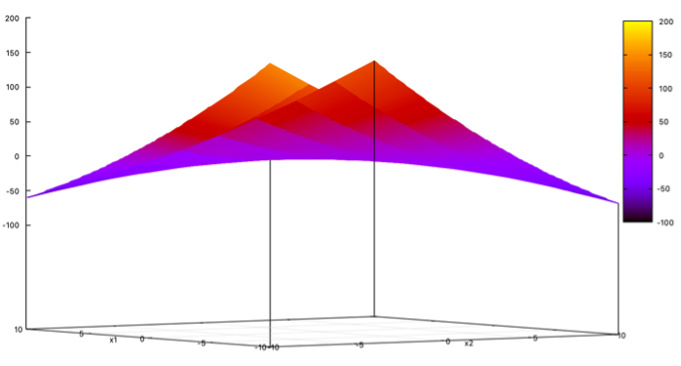
\includegraphics[width=1.0\textwidth]{L9-Duality-Gap-Example1.png}%
      \end{minipage}%
      \begin{minipage}{0.30\textwidth}
       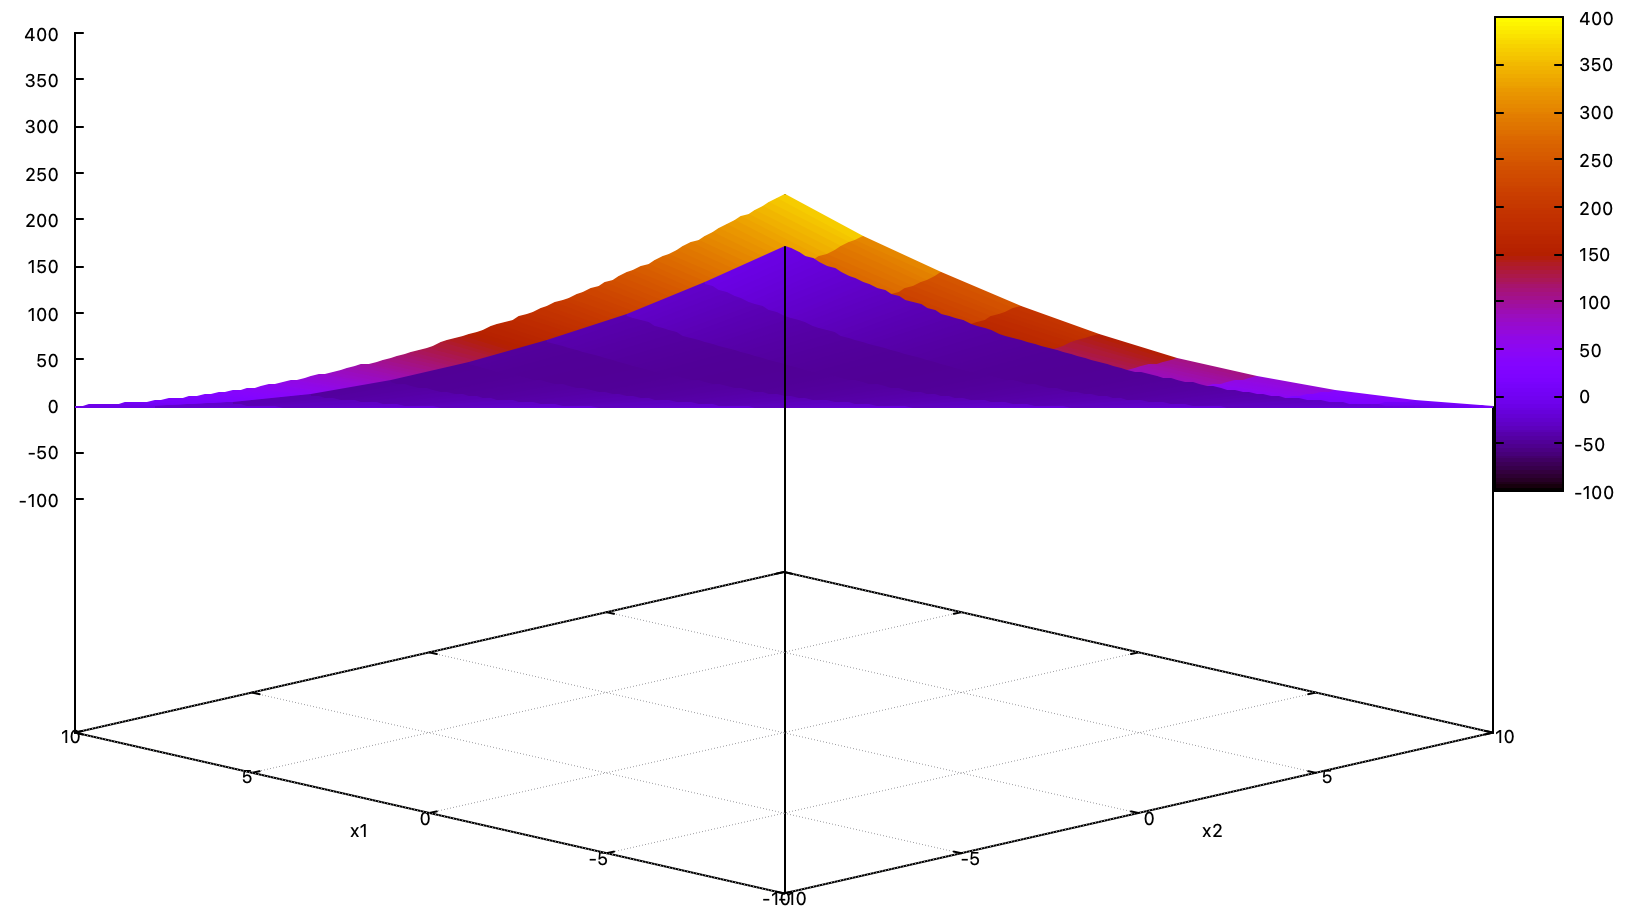
\includegraphics[width=1.0\textwidth]{L9-Duality-Gap-Example2.png}%
      \end{minipage}%
       \begin{minipage}{0.30\textwidth}
       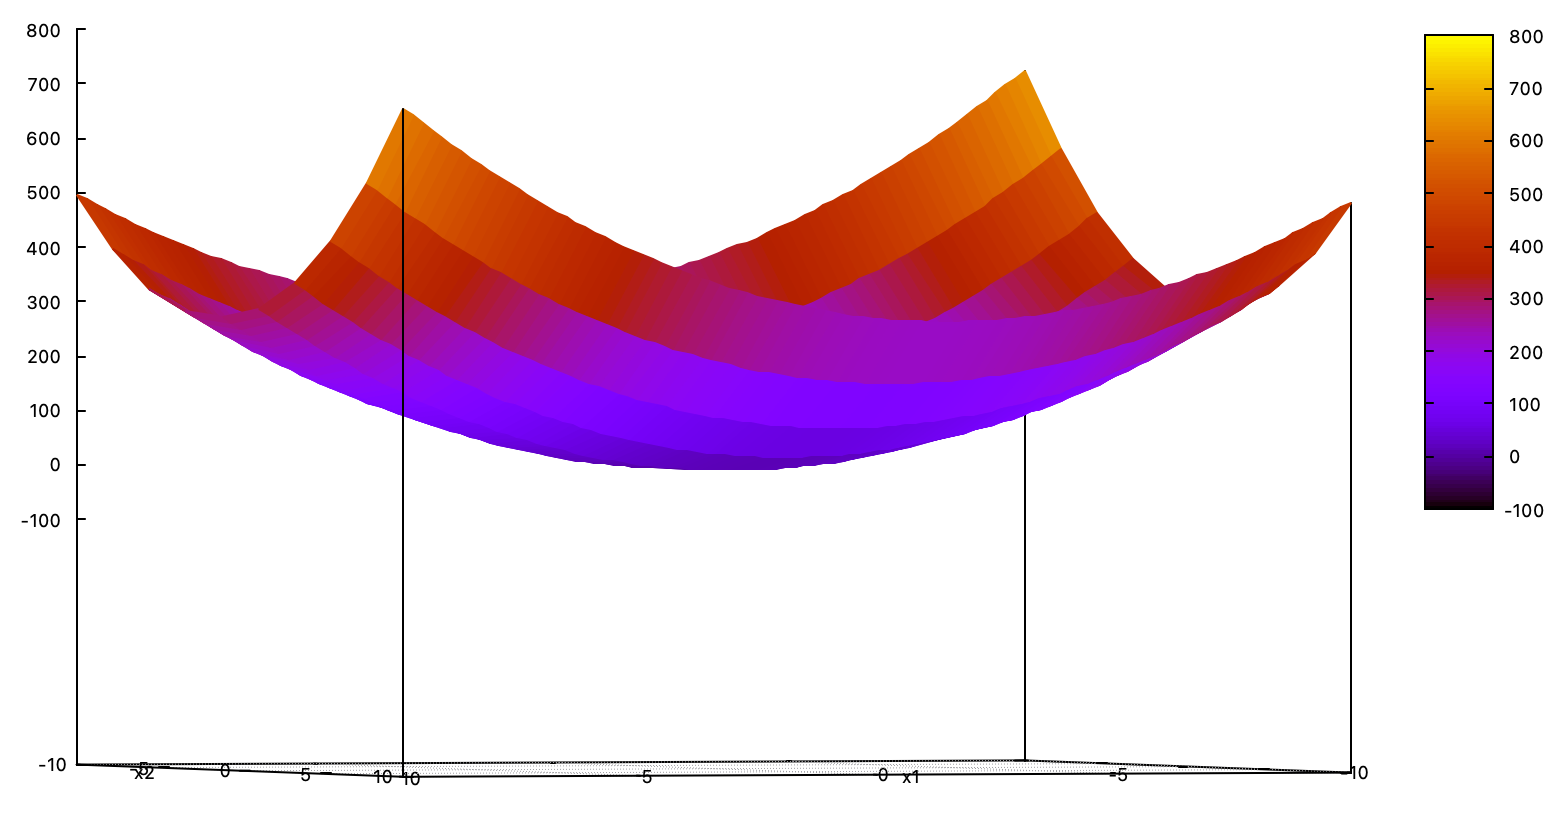
\includegraphics[width=1.0\textwidth]{L9-Duality-Gap-Example3.png}%
      \end{minipage}%
\end{figure}
	\item Lagrange dual function: 
\[
\begin{array}{lllll} 
	g(\lambda) &=&  \inf\limits_{x_1,x_2\in \mathbb{R} }  L(x_1, x_2, \lambda_1, \lambda_2, \lambda_3) \\
	&=&  
	 \begin{cases}  - \tfrac{1}{2} \left[\lambda_1 \lambda_2 \right] \left[ \begin{matrix}  2\lambda_3 & 1 \\ 1 & 2\lambda_3 \end{matrix} \right]^{-1}  \left[ \begin{matrix} \lambda_1 \\ \lambda_2 \end{matrix}\right]   -\lambda_3 & \text{if } \lambda_3 > \tfrac{1}{2} \\  
	 	 				 \tfrac{1}{2} & \text{if }  \lambda_3 = \tfrac{1}{2}, \lambda_1=\lambda_2 \\
	 	 				-\infty & \text{otherwise} \\

	 \end{cases} 
\end{array}
\]		
(This can be easily achieved by setting the gradient to be 0 in the case of $\lambda_3 >  \tfrac{1}{2}  $)

	\item Dual problem: 
\[
\begin{array}{rlllll}
 \max &  - \tfrac{1}{2} \left[\lambda_1 \lambda_2 \right] \left[ \begin{matrix}  2\lambda_3 & 1 \\ 1 & 2\lambda_3 \end{matrix} \right]^{-1}  \left[ \begin{matrix} \lambda_1 \\ \lambda_2 \end{matrix}\right]   -\lambda_3   \\
s.t. 	& \lambda_1   \geq  0  \\
 	& \lambda_2  \geq  0  \\
  & \lambda_3  \geq   \tfrac{1}{2}   \\
 \end{array} \nonumber
\]	
\item Note that by symmetry, $\lambda_1 = \lambda_2$ at the maximum point. Thus the objective function can be rewritten as $ - \lambda_1^2 (2\lambda_3 - 1)  -\lambda_3$. 

\begin{figure}
       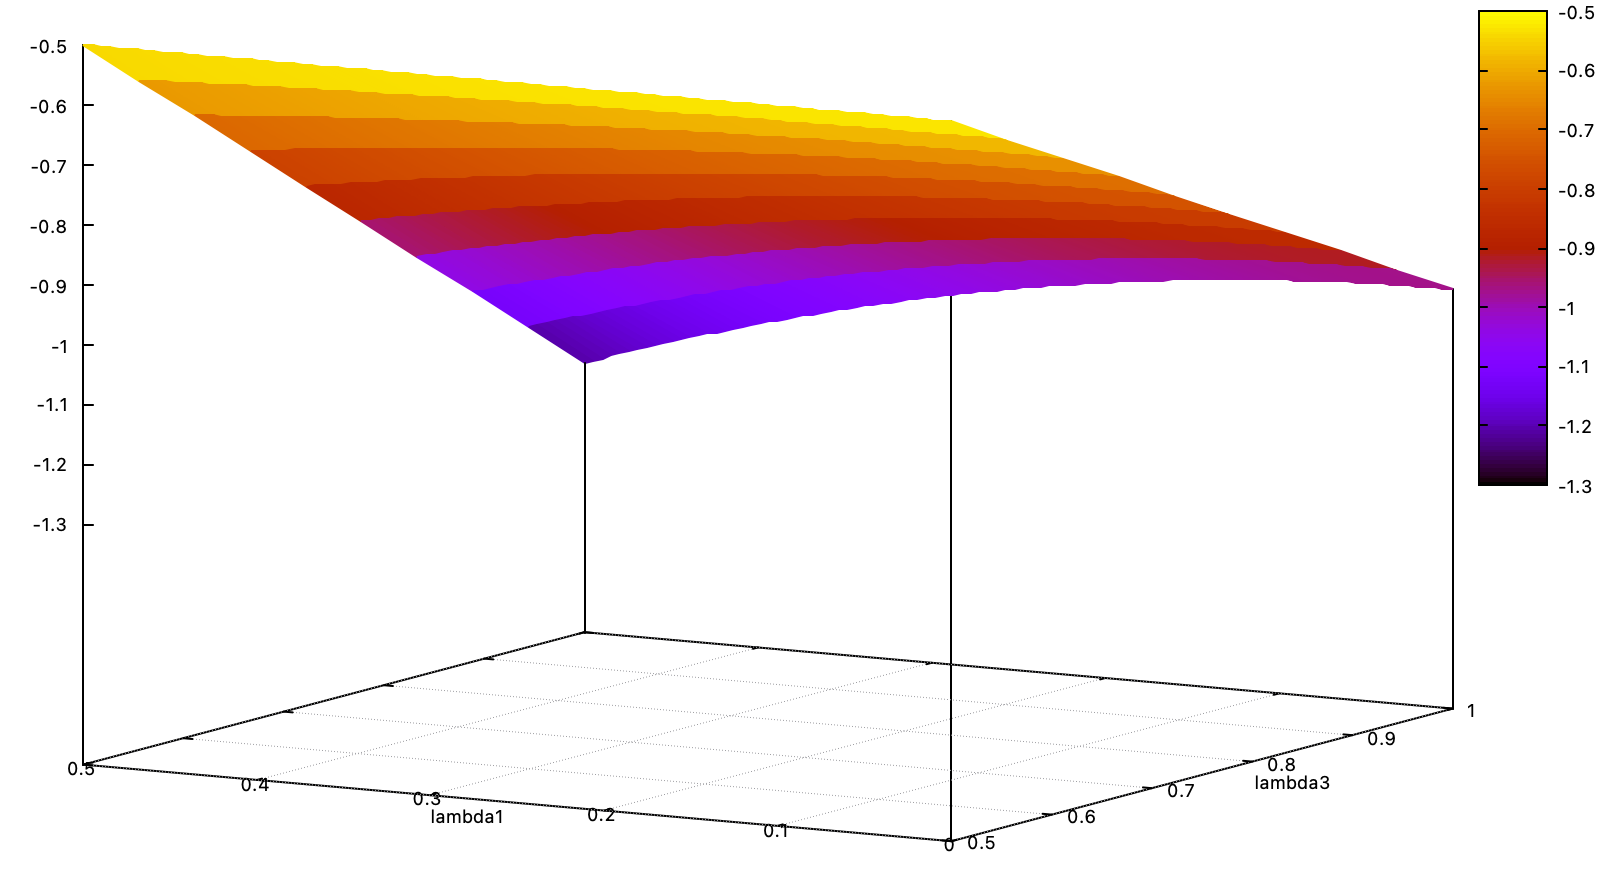
\includegraphics[width=0.5\textwidth]{L9-Duality-Gap-Example-g-lambda.png}%
\end{figure}

	\item Duality gap: $p^* = 0 > d^* = -\tfrac{1}{2}$. 
%	\item We will talk about Slater's condition later. 
\end{itemize}
	
}

\frame{
\begin{block}{}
Property of Lagrangian dual problem: Strong duality 
\end{block}
}

\frame{
	\frametitle{Strong duality} 
	
	\begin{itemize}
		\item Strong duality holds if $p^*=d^*$, i.e., the duality gap is 0. 
		\item Strong duality doesn't necessarily hold for any optimization problem, but it almost always holds for convex ones, i.e. 
\[
\begin{array}{rrrrrrrrl}
 \min &  f_0({x}) &   & &\\
 s.t.  & f_i({x})  & \leq &  0  & i=1, ..., m  \\
 	& {Ax}  & = &  {b} &  
 \end{array} \nonumber
\]
	where $f_i({x})$, $(i=0, 1, ..., m)$ are convex functions. 
	
	\item The conditions that guarantee strong duality are called \textcolor{red}{\bf regularity conditions}, one of which is the Slater's condition. 
	\end{itemize}
}

\frame{
	\frametitle{Slater's condition}
	
	\begin{itemize}
		\item Slater's condition: Consider a convex optimization problem. The strong duality holds if there exists a vector ${x} \in \mathbf{relint}\  \mathcal{D}$ such that 
\[
	f_i({x}) \textcolor{red}{\bf <} 0, i=1, ..., m, \quad {Ax = b } 
\]

		\item Suppose the first $k$ constraints are affine, then the Slater's conditions turns into: 
		there exists a vector ${x} \in \mathbf{relint} \mathcal{D}$ such that
\[
	f_i({x}) \textcolor{red}{\bf \leq} 0, i=1, ..., k, \quad f_i({x}) \textcolor{red}{\bf <} 0, i=1+1, ..., m, \quad {Ax = b } 
\]
	\item Specifically, if all constraints are affine, then the original constraints are themselves the Slater's conditions. 
	\item Please refer to Appendix for the proof of the Slater theorem. 
	\end{itemize}
}


\frame{
\begin{block}{}
Conditions of optimal solution: KKT conditions 
\end{block}
}


\frame{
\frametitle{Three types of optimization problems}
\begin{itemize}
 \item It is relatively easy to optimize an objective function \textcolor{red}{{\bf without any constraint}}, say: 
  \[
  \min\ f_0( {x} )
  \] 
  
 \item But how to optimize an objective function \textcolor{red}{{\bf with equality constraints}}? 
\[
\begin{array}{rrrrrrrrl}
 \min & f_0( {x})  &  & & \\
 s.t. & h_i( {x}) & \textcolor{red}{\bf =} &0 & i=1,2,..., p \\
\end{array} \nonumber
\]
\item And how to optimize an objective function  \textcolor{red}{{\bf with inequality constraints}}?
\[
\begin{array}{rrrrrrrrl}
 \min & f_0( {x})  &  & & \\
 s.t. & f_i( {x}) & \textcolor{red}{\bf \leq} &0  & i=1,2,..., m \\
       & h_i( {x}) & \textcolor{red}{\bf =} &0  & i=1,2,..., p 
\end{array} \nonumber
\]
\end{itemize} 
}

\frame{
\frametitle{Optimization problem over \textcolor{red}{\bf equality constraints} } 
\begin{itemize}
\item Consider the following optimization problem: 
\[
\begin{array}{rrrrrrrrl}
 \min & f_0(x,y)  &   &\\
 s.t. & h(x,y)  & \textcolor{red}{\bf =} & 0
\end{array} \nonumber
\]
 \item 
 Intuition: suppose $(x^{*}, y^{*})$ is the optimum point. Thus at $(x^{*}, y^{*})$, $f_0(x,y)$ does not change when  walking along the curve $h(x,y)=0$; 
  otherwise, we can follow the curve to make $f_0(x,y)$ smaller, meaning that the starting point $(x^{*}, y^{*})$ is not optimum. 
 \begin{figure}
\begin{tikzpicture}[scale=0.8, auto,swap]
 
 %\draw[<->,  thick] (0,4) node[thick, left]{$y$}-- (0,0) -- (4,0) node[ultra thick, below] {$x$};
\draw[dashed, blue] (1,1) circle[radius=1.8]; 
\draw[dashed, blue] (1,1) circle[radius=1];
%\draw[dashed, blue] (1,1) circle[radius=0.5];
%\draw[fill=blue] (1,1) circle[radius=1pt];

\draw[ultra thick, red!40] (0,4) to[out=280, in=180] (1,2) to[out=0, in=260] (2,4) node[red, right]{\small $h(x, y)=0$};

\draw[fill=blue] (1,2) circle[radius=1pt];

\node[black, ultra thick, below ] at (1.8,2) {\small $(x^*, y^*)$}; 
\draw[->,  thick, red!40] (1,2) -- (1.8, 2);
\draw[->,  thick, red] (1,2) -- (1, 2.7) node[above]{\small $\bigtriangledown h(x, y)$};
\draw[->, thick, blue] (1,2) -- (1, 1.3) node[below]{\small $\bigtriangledown f_0(x, y)$}; 
 
\node[blue, ultra thick ] at (1,-0.2) {\small  $f_0(x,y)=1$}; 
\node[blue, ultra thick] at (1,-1) {\small  $f_0(x,y)=2$}; 

        
\end{tikzpicture}
\end{figure}
  \end{itemize}
} 

\frame{
%\frametitle{Lagrangian multiplier: under \textcolor{red}{\bf equality constraints} } 
 \begin{figure}
\begin{tikzpicture}[scale=0.8, auto,swap]
 
 %\draw[<->,  thick] (0,4) node[thick, left]{$y$}-- (0,0) -- (4,0) node[ultra thick, below] {$x$};
\draw[dashed, blue] (1,1) circle[radius=1.8]; 
\draw[dashed, blue] (1,1) circle[radius=1];
%\draw[dashed, blue] (1,1) circle[radius=0.5];
%\draw[fill=blue] (1,1) circle[radius=1pt];

\draw[ultra thick, red!40] (0,4) to[out=280, in=180] (1,2) to[out=0, in=260] (2,4) node[red, right]{\small $h(x, y)=0$};

\draw[fill=blue] (1,2) circle[radius=1pt];

\node[black, ultra thick, below ] at (1.8,2) {\small $(x^*, y^*)$}; 
\draw[->,  thick, red!40] (1,2) -- (1.8, 2);
\draw[->,  thick, red] (1,2) -- (1, 2.7) node[above]{\small $\bigtriangledown h(x, y)$};
\draw[->, thick, blue] (1,2) -- (1, 1.3) node[below]{\small $\bigtriangledown f_0(x, y)$}; 
 
\node[blue, ultra thick ] at (1,-0.2) {\small  $f_0(x,y)=1$}; 
\node[blue, ultra thick] at (1,-1) {\small  $f_0(x,y)=2$}; 

        
\end{tikzpicture}
\end{figure}

\begin{itemize}
\item 
So at $(x^{*},y^{*})$, the red line tangentially touches a blue contour,  i.e. there exists a real $\lambda$ such that:  

\begin{center}
 $\bigtriangledown f_0(x, y) = \lambda \bigtriangledown h(x, y)$ 
\end{center}
%\[
%(\frac{\partial f(x,y) }{\partial x }, \frac{\partial f(x,y) }{\partial y }) = \lambda (\frac{\partial g(x,y) }{\partial x }, \frac{\partial g(x,y) }{\partial y })
%\]
\item Lagrange must have cleverly noticed that the equation above looks like partial derivatives of some larger scalar function: 

\begin{center}
$L(x,y,\lambda) = f_0(x,y) - \lambda h(x,y) $
\end{center}
\item Necessary conditions of optimum point: 
If $(x^{*}, y^{*})$ is local optimum, then there exists a  ${\lambda}$ such that 
$\bigtriangledown L(x^*, y^*, \lambda) = 0$.

\end{itemize}
} 

\frame{
\frametitle{Understanding Lagrangian function} 
\begin{itemize}

\item Lagrangian function: a combination of the original optimization objective function and constraints:  
\begin{center}
$L(x,y,\lambda) = f_0(x,y) - \lambda h(x,y) $
\end{center} 

%\item Here $\lambda g(x,y)$ can be treated as \textcolor{red}{\bf ``penalty of violating 
%constraints''} ---  $g(x,y)$ describes to what extent a constraint is violated, and $\lambda$ (called Lagrangian multiplier) describes the penalty weight. 

%\item Note   $\frac{\partial L(x,y,\lambda)}{\partial \lambda}  = 0 $ is essentially the equality constraint $h(x,y) = 0$. 

\item The critical point of Lagrangian $L(x, y, \lambda)$ occurs at saddle points rather than local minima (or maxima). Thus, to utilize numerical optimization techniques, we must first transform the problem such that the critical points lie at local minima. This is done by calculating the magnitude of the gradient of Lagrangian. 

\end{itemize}
}

%
%\frame{
%\frametitle{Intuition of Lagrangian multiplier technique}
%\begin{itemize}
%\item 
%Suppose $(x^{*},y^{*})$ is the optimum point of the original  problem with constraints; 
%\item 
%Draw the contour map of $f(x,y)$ (in blue) and the curve $g(x,y)=c$ (in red); 
%
%\item Thus, we have: 
%$\frac{\partial L(x,y,\lambda)}{\partial x }|_{(x^{*},y^{*})} = 0$ 
%and 
%$\frac{\partial L(x,y,\lambda)}{\partial y }|_{(x^{*},y^{*})} = 0$
%\end{itemize}
%
%\begin{figure}
% \includegraphics[width=1.9in] {L8-Lagrangian.png}
%\end{figure}
%}

\frame{
\frametitle{Optimization problems over  \textcolor{red}{\bf inequality constraints} } 
\begin{itemize}
\item Consider the following optimization problem: 
\[
\begin{array}{rrrrrrrrl}
 \min & f_0( x, y)  &   & \\
 s.t. & f_1(  x, y)  &\textcolor{red}{\bf \leq} & 0 & \\
 %      & h_i( {x})  &\textcolor{red}{\bf \leq} & 0 & i=1,2,..., p
\end{array} \nonumber
\]
\end{itemize}
\begin{figure}
\begin{minipage}{0.49\textwidth}
\begin{tikzpicture}[scale=0.8, auto,swap]
 
 %\draw[<->,  thick] (0,4) node[thick, left]{$y$}-- (0,0) -- (4,0) node[ultra thick, below] {$x$};
\draw[white, fill=gray!15] (0,4) to[out=280, in=180] (1,2) to[out=0, in=260] (2,4) -- (0,4);
\draw[ultra thick, red!40] (0,4) to[out=280, in=180] (1,2) to[out=0, in=260] (2,4); 
\node[ultra thick, red] at (1, 4.0) {\small $f_1(x, y)\leq 0$}; 

\draw[dashed, blue] (1,1) circle[radius=1.8]; 
\draw[dashed, blue] (1,1) circle[radius=1];

%\draw[fill=blue] (1,1) circle[radius=1pt];


\draw[fill=blue] (1,2) circle[radius=1pt];

 \node[black, ultra thick, below ] at (0.85,2) {\small $(x^*, y^*)$}; 
%\draw[->,  thick, red!40] (1,2) -- (1.8, 2);
%\draw[->,  thick, red] (1,2) -- (1, 2.7) node[above]{\small $\bigtriangledown g(x, y)$};
 %\draw[->, thick, blue] (1,2) -- (1, 1.3) node[below]{\small $\bigtriangledown f(x, y)$}; 
 
  \node[blue, ultra thick ] at (1,-0.2) {\small  $f_0( x, y)=1$}; 
 \node[blue, ultra thick] at (1,-1) {\small  $f_0( x, y)=2$}; 

        
\end{tikzpicture}
\end{minipage}
\begin{minipage}{0.49\textwidth}
\begin{tikzpicture}[scale=0.8, auto,swap]
 
 %\draw[<->,  thick] (0,4) node[thick, left]{$y$}-- (0,0) -- (4,0) node[ultra thick, below] {$x$};
\draw[white, fill=gray!15] (0,4-1.8) to[out=280, in=180] (1,2-1.8) to[out=0, in=260] (2,4-1.8) -- (0,4-1.8);
\draw[ultra thick, red!40] (0,4-1.8) to[out=280, in=180] (1,2-1.8) to[out=0, in=260] (2,4-1.8); 
\node[ultra thick, red] at (1,3.5-1.2) {\small $f_1(x, y)\leq 0$}; 

\draw[dashed, blue] (1,1) circle[radius=1.8]; 
\draw[dashed, blue] (1,1) circle[radius=1];
\draw[dashed, blue] (1,1) circle[radius=0.4];

\draw[fill=blue] (1,1) circle[radius=1pt];


%\draw[fill=blue] (1,2) circle[radius=1pt];

 \node[black, ultra thick, below ] at (0.85,1) {\small $(x^*, y^*)$}; 
%\draw[->,  thick, red!40] (1,2) -- (1.8, 2);
%\draw[->,  thick, red] (1,2) -- (1, 2.7) node[above]{\small $\bigtriangledown g(x, y)$};
 %\draw[->, thick, blue] (1,2) -- (1, 1.3) node[below]{\small $\bigtriangledown f(x, y)$}; 
 
  \node[blue, ultra thick ] at (1,-0.2) {\small  $f_0(x, y)=1$}; 
 \node[blue, ultra thick] at (1,-1) {\small  $f_0(x, y)=2$}; 

        
\end{tikzpicture}
\end{minipage}
\caption{Case 1: the optimum point $(x^*, y^*)$ lies in the curve $f_1(x, y) =0$. Thus Lagrangian condition $\bigtriangledown L(x, y, \lambda) = {0}$ applies.  Case 2: $(x^*, y^*)$ lies within the interior region $f_1(x, y) \textcolor{red}{<} 0$; thus we have $\bigtriangledown f_0(x, y) = 0$ at $(x^*, y^*)$}.
\end{figure}
} 


\frame{
	\frametitle{\textcolor{red}{\bf Complementary slackness}}
	
%\begin{figure}
%\begin{minipage}{0.49\textwidth}
%\begin{tikzpicture}[scale=0.8, auto,swap]
% 
% %\draw[<->,  thick] (0,4) node[thick, left]{$y$}-- (0,0) -- (4,0) node[ultra thick, below] {$x$};
%\draw[white, fill=gray!15] (0,4) to[out=280, in=180] (1,2) to[out=0, in=260] (2,4) -- (0,4);
%\draw[ultra thick, red!40] (0,4) to[out=280, in=180] (1,2) to[out=0, in=260] (2,4); 
%\node[ultra thick, red] at (1, 4.0) {\small $f_1(x, y)\leq 0$}; 
%
%\draw[dashed, blue] (1,1) circle[radius=1.8]; 
%\draw[dashed, blue] (1,1) circle[radius=1];
%
%%\draw[fill=blue] (1,1) circle[radius=1pt];
%
%
%\draw[fill=blue] (1,2) circle[radius=1pt];
%
% \node[black, ultra thick, below ] at (0.85,2) {\small $(x^*, y^*)$}; 
%%\draw[->,  thick, red!40] (1,2) -- (1.8, 2);
%%\draw[->,  thick, red] (1,2) -- (1, 2.7) node[above]{\small $\bigtriangledown g(x, y)$};
% %\draw[->, thick, blue] (1,2) -- (1, 1.3) node[below]{\small $\bigtriangledown f(x, y)$}; 
% 
%  \node[blue, ultra thick ] at (1,-0.2) {\small  $f_0( x, y)=1$}; 
% \node[blue, ultra thick] at (1,-1) {\small  $f_0( x, y)=2$}; 
%
%        
%\end{tikzpicture}
%\end{minipage}
%\begin{minipage}{0.49\textwidth}
%\begin{tikzpicture}[scale=0.8, auto,swap]
% 
% %\draw[<->,  thick] (0,4) node[thick, left]{$y$}-- (0,0) -- (4,0) node[ultra thick, below] {$x$};
%\draw[white, fill=gray!15] (0,4-1.8) to[out=280, in=180] (1,2-1.8) to[out=0, in=260] (2,4-1.8) -- (0,4-1.8);
%\draw[ultra thick, red!40] (0,4-1.8) to[out=280, in=180] (1,2-1.8) to[out=0, in=260] (2,4-1.8); 
%\node[ultra thick, red] at (1,3.5-1.2) {\small $f_1(x, y)\leq 0$}; 
%
%\draw[dashed, blue] (1,1) circle[radius=1.8]; 
%\draw[dashed, blue] (1,1) circle[radius=1];
%\draw[dashed, blue] (1,1) circle[radius=0.4];
%
%\draw[fill=blue] (1,1) circle[radius=1pt];
%
%
%%\draw[fill=blue] (1,2) circle[radius=1pt];
%
% \node[black, ultra thick, below ] at (0.85,1) {\small $(x^*, y^*)$}; 
%%\draw[->,  thick, red!40] (1,2) -- (1.8, 2);
%%\draw[->,  thick, red] (1,2) -- (1, 2.7) node[above]{\small $\bigtriangledown g(x, y)$};
% %\draw[->, thick, blue] (1,2) -- (1, 1.3) node[below]{\small $\bigtriangledown f(x, y)$}; 
% 
%  \node[blue, ultra thick ] at (1,-0.2) {\small  $f_0(x, y)=1$}; 
% \node[blue, ultra thick] at (1,-1) {\small  $f_0(x, y)=2$}; 
%
%        
%\end{tikzpicture}
%\end{minipage}
%\caption{Case 1: the optimum point lies in the curve $f_1(x, y) =0$. Thus Lagrangian condition $\bigtriangledown L(x, y, \lambda) = {0}$ applies.  Case 2: the optimum point lies within the region $f_1(x, y) \leq 0$; thus we have $\bigtriangledown f_0(x, y) = 0$ at $(x^*, y^*)$}.
%\end{figure}
\begin{itemize}
\item 
These two cases can be  summarized as the following two conditions: 
\begin{itemize}
\item (Stationary point) $\bigtriangledown L({x^*, y^*, \lambda }) = {0}$
\item (Complementary slackness) $\lambda f_1( {x^*, y^*}) = 0$
\end{itemize} 
\item Reason: In case 2, $f_i({x^*}) \textcolor{red}{<} 0 \Rightarrow  \lambda = 0 $ by complementary slackness. We further have $\bigtriangledown f_0({x^*, y^*}) = 0$ since $\bigtriangledown L({x^*, y^*, \lambda }) = {0}$. 
		\item Complementary slackness, also called \textcolor{red}{\bf orthogonality} by Gomory, essentially equals to the strong duality for convex optimization problems. 
		\item A relaxation of this condition, i.e., $\lambda_i f_i( {x^*}) = \mu$, where $\mu$ is a small positive number,  is used in the interior point method. 
\end{itemize}

}

\frame{
	\frametitle{Proof of complementary slackness}
	\begin{itemize}
		\item Assume that strong duality holds, i.e., $p^*=d^*$. Let's $x^*$ and $(\lambda^*, \nu^*)$ $\lambda^*\leq 0$ denote the optimal solution to the primal problem and dual problem, respectively. We have: 
	\begin{eqnarray}
		f_0(x^*) & = & g(\lambda^*, \nu^*) \nonumber\\
			&=& \inf\limits_{x\in \mathcal{D}} (f_0(x) - \sum\nolimits_{i=1}^m \lambda_i f_i(x) - \sum\nolimits_{i=1}^p \nu_i h_i(x) ) \nonumber\\
			&\leq& f_0(x^*) - \sum\nolimits_{i=1}^m \lambda_i f_i(x^*) - \sum\nolimits_{i=1}^p \nu_i h_i(x^*) 			\nonumber\\
			&\leq& f_0(x^*) \nonumber
	\end{eqnarray}

	\item Thus the last two inequalities turns into equalities, which implies that Lagrangian function $L(x, \lambda^*, \nu^*)$ reaches its minimum at $x^*$ and 
\[
	\sum\nolimits_{i=1}^m \lambda_i^* f_i(x^*) = 0. 
\]	
	\item Note that $\lambda_i^* f_i(x^*) \geq 0$. Hence $\lambda_i^* f_i(x^*) = 0$ for $i=1,..., m$. 
	\end{itemize}

}
%\frame{
%	\frametitle{Understanding \textcolor{red}{\bf complementary slackness}  (cont'd) }
%	
%	\begin{itemize}
%		\item Complementary slackness, also called {\it orthogonality} by Gomory, essentially equals to the strong duality, i.e., the primal and dual problems have identical objective value. 
%
%		\item 
%Complementary slackness says that at an optimum point, if a shadow price (dual variable) is positive, meaning that the objective function could be increased if the corresponding primal constraint was relaxed, then this primal constraint must be tight. Otherwise, the primal objective function value could be improved (by changing the primal variables in order to make this non-binding primal constraint binding).
%
%	\end{itemize}
%
%}


%\frame{
%\frametitle{KKT conditions}
%\begin{itemize}
% \item Consider an optimization problem with its Lagrangian function 
% \[
% L({x, \lambda }) = f_0({x}) - \sum_{i=1}^m \lambda_i f_i({x}) 
% \]
% %- \sum_{i=1}^k \nu_i h_i({x})
% 
%\item Necessary conditions of optimum point: \\
%If ${x^*}$ is local optimum and the primal problem satisfies some regularity conditions (say Slater's conditions), then there exists ${\lambda}$ such that: 
%\begin{enumerate}
%\item (Stationary point) $\bigtriangledown L({x^*, \lambda }) = {0}$
%\item (Primal feasibility) $f_i({x^*}) \leq 0$, $i=1, ..., m$
%\item (Dual feasibility) $\lambda_i \leq 0$, $i=1, ..., m$
%\item (Complementary slackness) $\lambda_i f_i( {x^*}) = 0$, $i=1, ..., m$
%\end{enumerate}
%\item KKT conditions are usually not solved directly in optimization; instead, iterative successive approximation is most often used to find the final results that satisfy KKT conditions. 
%\end{itemize}
%\footnote{\tiny KKT conditions were named after William Karush, Harold W. Kuhn, and Albert W. Tucker.}
%}


\frame[allowframebreaks]{
	\frametitle{KKT conditions for general optimization problems }
	
	\begin{itemize}
			\item Consider the following constrained optimization problem (might be non-convex). 
\[
\begin{array}{rlllllllll}
 \min & f_0({x}) & &   &\\
 s.t. & f_i({x}) & \leq& 0 & i=1, ..., m\\ 
  	& h_i({x}) & =& 0 & i=1, ..., p\\ 
\end{array} \nonumber
\]
		\item Lagrangian function: 
 \[
 L({x, \lambda }) = f_0({x}) - \sum_{i=1}^m \lambda_i f_i({x}) - \sum_{i=1}^k \nu_i h_i({x}) 
 \]
% where ${\lambda} \leq 0$. 
		\item Let ${x^*}$ and $({\lambda}, {\nu})$ denote the optimal solutions to the primal and dual problems, respectively. Suppose the strong duality holds. 
		\item Since Lagrangian function reaches its minimum at ${x^*}$,  its gradient is 0 at ${x^*}$, i.e., 
\[
	\bigtriangledown f_0({x^*}) - \sum_{i=1}^{m} \lambda_i \bigtriangledown f_i({x^*}) - \sum_{i=1}^k \nu_i \bigtriangledown h_i({x^*}) = 0
\]		
		\item Then ${x^*}$ and $({\lambda, \nu})$ satisfy the following KKT conditions: 

\begin{enumerate}
\item (Stationary point) $\bigtriangledown L({x^*, \lambda, \nu}) = {0}$
\item (Primal feasibility) $f_i({x^*}) \leq 0$, $i=1,  ..., m$; $h_i({x^*}) = 0$, $i=1,  ..., p$
\item (Dual feasibility) $\lambda_i \leq 0$, $i=1, ..., m$
\item (Complementary slackness) $\lambda_i f_i( {x^*}) = 0$, $i=1,  ..., m$
\end{enumerate}
		
	\end{itemize}
 
}


\frame[allowframebreaks]{
	\frametitle{KKT conditions for convex problems }
	
	\begin{itemize}
			\item Consider the following convex optimization problem. 
\[
\begin{array}{rlllllllll}
 \min & f_0({x}) & &   &\\
 s.t. & f_i({x}) & \leq& 0 & i=1, ..., m\\ 
  	& {Ax} & =& {b} & \\ 
\end{array} \nonumber
\]
		\item Lagrangian function: 
 \[
 L({x, \lambda }) = f_0({x}) - \sum_{i=1}^m \lambda_i f_i({x}) -  { \nu^T (Ax - b)} 
 \]
% where ${\lambda} \leq 0$. 
\ \\
\ \\
\ \\
\ \\
\ \\
\ \\
\ \\
\ \\
		\item ${x^*}$ and $(\lambda, \nu)$ are optimal solutions to the primal and dual problems, respectively, if they satisfy the following KKT conditions: 

\begin{enumerate}
\item (Stationary point) $\bigtriangledown L({x^*, \lambda, \nu }) = {0}$
\item (Primal feasibility) $f_i({x^*}) \leq 0$, $i=1, ..., m$; ${Ax} =b$; 
\item (Dual feasibility) $\lambda_i \leq 0$, $i=1, ..., m$
\item (Complementary slackness) $\lambda_i f_i( {x^*}) = 0$, $i=1, ..., m$
\end{enumerate}

		\item KKT conditions, named after William Karush, Harold W. Kuhn, and Albert W. Tucker,  are usually not solved directly in optimization; instead, iterative successive approximation is most often used to find the final results that satisfy KKT conditions. 

	\end{itemize}
 
}



%
%\frame{
%\frametitle{Lagrangian $L(x,\lambda)$: connecting primal variable $x$ and dual variable $\lambda$ } 
%\begin{itemize}
% \item Primal problem: 
%\[
%\begin{array}{rrrrrrrrl}
% \min & x^2  &   \\
% s.t. & x \leq  2 \\
%\end{array} \nonumber
%\]
% \item Lagrangian: $L(x,\lambda) = x^2 - \lambda (x-2)$
% \item For any $x\leq 0$, $\lambda  \leq 0$, we have $x^{2}  \geq  L(x, \lambda)$. 
% \item The optimum is a saddle point of $L(x,\lambda)$z.
% \end{itemize}
%
%\begin{figure}
% \includegraphics[width=2.in,angle=-90] {L9-Lagrangian-duality-example1.eps}
%\end{figure}
%
%}


%
%\frame{
%\begin{block}{}
%Lagrangian multiplier technique and KKT conditions
% \end{block}
%}




\frame{
\begin{block}{}
 Four properties of duality for linear program
\end{block}
}

\frame{
\frametitle{Property 1: Primal is the dual of dual  }
\begin{Theorem}
For linear program, primal problem is the dual of dual. 
\end{Theorem}
\begin{itemize}
	\item For a general optimization problem, the dual of dual is not always the primal problem but a convex relaxation of the primal problem.
\end{itemize}

} 

\frame{
\frametitle{Property 2: Weak duality }
\begin{Theorem}
\textit{(Weak duality)} The objective value of \textcolor{red}{\bf any} feasible solution to the  dual problem is always a lower bound of  the objective value of primal problem.  
\end{Theorem}

%\begin{figure}
% \includegraphics[width=2.4in,angle=-90] {L9-Lagrangian-dual.eps}
%\end{figure}

\begin{itemize}
	\item It is easy to prove this property as  Lagrangian function connects  primal objective function and dual objective function. 
\end{itemize}

} 

\frame{
\frametitle{An example: {\sc Diet} problem and its dual problem  }
\begin{small}
\begin{itemize}
\item 
Primal problem $P$: 
\[
\begin{array}{rrrrrrrrlr}
 \min & 3x_1   &+& 9 x_2   &+& 20x_3   &+& 19x_4   & & \text{money}\\
 s.t. & 110x_1 &+& 160 x_2 &+& 420 x_3 &+& 260 x_4 & \geq 2000 & \text{energy} \\
      & 4 x_1  &+& 8 x_2   &+& 4 x_3   &+& 14 x_4  & \geq 55 & \text{protein}\\
      &  2 x_1 &+& 285 x_2 &+& 22 x_3  &+& 80 x_4  & \geq 800 & \text{calcium}\\
      & x_1    &,& x_2     &,& x_3     &,&    x_4  & \geq 0 \\ 		
\end{array} \nonumber
\] 
Feasible solution ${ x^T}=[0, 8, 2, 0]^T\Rightarrow { c^Tx}=112$. 
\item 
Dual problem $D$:  
\[
\begin{array}{rrrrrrlr}
 \max & 2000 y_1   &+& 55 y_2   &+& 800 y_3 & & \text{money}   \\
 s.t. & 110 y_1 &+& 4 y_2 &+& 2 y_3   & \leq 3 & \text{oatmeal} \\
      & 160 y_1 &+& 8 y_2 &+& 285 y_3 & \leq 9 & \text{milk} \\
      & 420 y_1 &+& 4 y_2 &+& 22 y_3  & \leq 20 & \text{pie} \\
      & 260 y_1 &+& 14 y_2 &+& 80 y_3  & \leq 19 & \text{pork\&beans} \\
      &     y_1 &,&    y_2 &,&    y_3  &  \geq 0 \\ 		
\end{array} \nonumber
\]
Feasible solution ${ y^T}=[0.0269, 0, 0.0164]^T\Rightarrow { y^Tb}=67.096$
\item 
The theorem states that ${ c^Tx \geq y^T b}$ for \textcolor{red}{\bf  any} feasible solutions ${ x }$ and ${ y }$. 
\end{itemize}
\end{small}
} 

\frame{
\frametitle{}
\begin{Proof}
\begin{itemize}
\item Consider the following {\sc Primal} problem: 
\begin{small}
\[
\begin{array}{rrrrrrrrl}
 \min & {c^T x}  &  & \\
 s.t.  & {A x } &  \geq &  {b }  \\
 	& {x  } &  \geq & {0 } 
 \end{array} \nonumber
\]
\end{small}
and {\sc Dual} problem: 
\begin{small}
\[
\begin{array}{rrrl}
 \max & {b^T y} &   & \\
 s.t. & {y}  &  \geq & 0   \\
      & {A^T y} &   \leq  & {c } 
\end{array} \nonumber
\]
\end{small}
 \item 
Let ${x}$ and ${y}$ denote a feasible solution to primal and dual problems, respectively. 
\item 
We have ${c^T x \geq y^T A  x }$ (by the feasibility of dual problem, i.e., ${y^T A \leq c^T}$, and ${x^T \geq 0}$ )
\item 
Therefore ${c^T x \geq y^T A  x \geq y^T b }$ (by the feasibility of primal problem, i.e., ${Ax \geq b}$, and ${y \geq 0}$) 
\end{itemize}
\end{Proof}

}

\frame{
\frametitle{Property 3: Strong duality }

\begin{Theorem}
\textit{(Strong duality)} Consider a linear program. If the primal problem has an optimal solution, then the dual problem also has an optimal solution with the same objective value. 
\end{Theorem}
\begin{Proof}
\begin{itemize}
\item Suppose ${x^*= \left[ \begin{array}{c} {B}^{-1}b\\ 0 \end{array}\right]}$ be the optimal solution to the primal problem. We have ${c^T - c_B^T B^{-1} A \geq 0}$. 
\item Let's set \textcolor{red}{${y^{*T}={c_B}^T {B}^{-1}}$}.  We will show that ${y^{*T}}$ is the optimal solution to the dual problem.
\item In fact, we have ${y^{*T} b = {c_B}^T {B}^{-1} b = {c}^T {x^*}}$. 
\item That is, ${y^{*T}b}$ reaches its upper bound. So ${y^{*T}}$ is an optimal solution to the dual problem. \end{itemize}
\end{Proof}
\begin{footnotesize}
\end{footnotesize}
}


\frame{
\frametitle{Property 4: Complementary slackness}

% Primal: 
% \[
% \begin{array}{rrrrrrrrl}
%  \min & c^T x &   \\
%  s.t. & A_i^T x = b_i & i\in M \\
%       & A_i^T x \geq b_i & i \in \overline{M} \\
%       & x_i \geq 0 & i \in N \\
%       & x_i \leq\geq 0 & i \in \overline{N}\\
% \end{array} \nonumber
% \]
% 
% Dual problem: 
% \[
% \begin{array}{rrrrrrrrl}
%  \max & y^T  &   \\
%  s.t. & y_i \leq\geq 0 & i\in M \\
%       & y_i \geq 0 & i \in \overline{M} \\
%       & y^T A_i \leq  c_i & i \in N \\
%       & y^T A_i = c_i  & i \in \overline{N}\\
% \end{array} \nonumber
% \]

\begin{Theorem}
Let ${x}$ and ${y}$ denote feasible solutions to the primal and dual problems, respectively. Then ${x}$ and ${y}$ are optimal solutions iff 
$u_i =   y_i ( a_{i1}x_{1} + a_{i2}x_{2} + ... +a_{in}x_{n}  - b_i) = 0$ for any $1\leq i \leq m$, and\\
$v_j =  ( c_j - a_{1j}y_{1} - a_{2j}y_{2} - ... - a_{mj}y_{m} )x_j = 0$ for any $1\leq j \leq n$.
\end{Theorem}

\begin{itemize} 
\item Intuition: a constraint of primal problem is loosely restricted $\Rightarrow$ the  corresponding  dual variable is tight. 
\item An example: the optimal solutions to {\sc Diet} and its dual are ${x}=(14.244, 2.707, 0, 0 )$ and ${y}=(0.0269, 0, 0.0164)$.
\[
\begin{array}{rrrrrrrrlr}
 & 110x_1 &+& 160 x_2 &+& 420 x_3 &+& 260 x_4 & \textcolor{red}{=} 2000 & \\
      & 4 x_1  &+& 8 x_2   &+& 4 x_3   &+& 14 x_4  & \textcolor{red}{>} 55 & \textcolor{red}{\Rightarrow y_2=0}\\
      &  2 x_1 &+& 285 x_2 &+& 22 x_3  &+& 80 x_4  & \textcolor{red}{=} 800 & \\
      & x_1    &,& x_2     &,& x_3     &,&    x_4  & \geq 0 \\ 		
\end{array} \nonumber
\] 
\end{itemize}
} 

\frame{
\frametitle{Proof}
\begin{Proof}

$ u_i = 0 \text{ and }  v_j = 0 $ for any $i$ and $j$\\
$ \Leftrightarrow \sum_i u_i = 0 \text{ and } \sum_j v_j = 0 \text{ (since } u_i \geq 0, v_j \geq 0\text{)} $ \\
$ \Leftrightarrow  \sum_i u_i + \sum_j v_j = 0 $ \\
$\Leftrightarrow  { ( y^T A x - y^T b )+ ( c^T x - y^T A x ) = 0}  $\\
$\Leftrightarrow  { y^T b = c^T x } $\\
$\Leftrightarrow  {y}  \text{ and } {x}$  are optimal solutions (by strong duality property, i.e., both ${y^T b}$ and ${c^T x}$ reach its bound)

\end{Proof}
}

\frame{
\frametitle{Summary: 9 cases of primal and dual problems}

\begin{figure}
 \includegraphics[width=4in] {L9-primaldual-table.png}
\end{figure}
}

\frame{
	\frametitle{Example 1: {\sc Primal} has unbounded objective value and {\sc Dual} is infeasible } 
{\sc Primal}:
\[
\begin{array}{rrrrrrl}
 \min & -2 x_1 & - & 2x_2 & \\
 s.t. &   x_1 & - & x_2 & \leq & 1   \\
      & - x_1 & + & x_2 & \leq & 1   \\
      &   x_1 &   &         & \geq & 0   \\
            &      &  & x_2 & \geq & 0   
\end{array} \nonumber
\]
\ \\
\ \\
{\sc Dual}:
\[
\begin{array}{rrrrrrl}
 \max & y_1 & + & y_2 & \\
 s.t. &   y_1 & &         &       \leq & 0   \\
      &   &       &    y_2     & \leq & 0   \\
      &   y_1 & - & y_2  & \leq & -2   \\
      &   -y_1 &+ & y_2 & \leq & -2   \\
\end{array} \nonumber
\]
}


\frame{
	\frametitle{Example 2: both  {\sc Primal} and {\sc Dual} are infeasible } 
{\sc Primal}:
\[
\begin{array}{rrrrrrl}
 \min &   x_1 & - & 2x_2 & \\
 s.t. &   x_1 & - & x_2 & \geq & 2   \\
      & - x_1 & + & x_2 & \geq & -1   \\
      &   x_1 &   &         & \geq & 0   \\
            &      &  & x_2 & \geq & 0   
\end{array} \nonumber
\]
\ \\
\ \\
{\sc Dual}:
\[
\begin{array}{rrrrrrl}
 \max & 2y_1 & - & y_2 & \\
 s.t. &   y_1 & &         &       \geq & 0   \\
      &   &       &    y_2     & \geq & 0   \\
      &   y_1 & - & y_2  & \leq & 1   \\
      &   -y_1 &+ & y_2 & \leq & -2   \\
\end{array} \nonumber
\]
}



\frame{
\begin{block}{}
Solving linear program using duality 
\end{block}
}

\frame{
	\frametitle{KKT conditions for linear program} 
	
	\begin{itemize}
		\item Consider a linear program in slack form and its dual problem: 
\[
\begin{array}{rrrrrrlrrrrrl}
 \min &   {c^Tx} &  &              &\quad &   \max & {b^T y}  & &  \\
 s.t. &   {Ax} & = & {b}            & &   s.t.    &   y^T A  &\leq& c^T \\
      & {x}      & \geq & 0          & &            &        &.     &
\end{array} \nonumber
\]		The KKT conditions turns into: 
		${x}$ and ${y}$ are optimal solutions to the primal and dual problems, respectively, if they satisfy the following three conditions: 
		\begin{enumerate}
			\item \textcolor{red}{\bf (Primal feasibility)} 
		\[
			{Ax = b }, {x \geq 0} 
		\]	
			\item \textcolor{green}{\bf(Dual feasibility)} 
		\[
			{y^TA \leq c^T } 
		\]	

			\item \textcolor{blue}{\bf(Complementary slackness)} 
		\[
			{c^T x = y^T b }
		\]		
		\end{enumerate}
		
		\item Question: How to obtain ${x}$ and ${y}$ that satisfy these three conditions simultaneously? 
	\end{itemize}
}

\frame{
	\frametitle{{\sc Improvement} framework} 

\begin{itemize}
	\item We could start with an initial value of $x$ and $y$ that satisfy two constraints, and attempt to improve them  to reduce the unsatisfiability of the third constraint. This improvement steps will be repeated until all of the three constraints are satisfied. 
\end{itemize}
	
\begin{algorithmic}[1]
\STATE Initialize ${(x, y)}$ with values that satisfy two constraints; 
\WHILE{\texttt{TRUE}}
	\STATE{Improve $x$ and $y$ to reduce the unsatisfiability of the third constraint. }   
	\IF{all the three constraints are satisfied} 
		\STATE break;
	\ENDIF
\ENDWHILE
\RETURN ${(x, y)}$;
\end{algorithmic}
}


\frame{
	\frametitle{Strategy 1} 
	
\begin{algorithmic}[1]
\STATE ${x=x_0}$;  //Initialize ${x}$ with  a \textcolor{red}{\bf primal feasible solution}    
\STATE ${y=y_0}$; //Calculate initial ${y}$ according to  \textcolor{blue}{\bf complementary slackness}
\WHILE{\texttt{TRUE}}
	\STATE ${x}=${\sc Improve}$({x})$; 
	\STATE{//Improve ${x}$ to  \textcolor{green}{\bf reduce dual infeasibility of corresponding $y$}. Throughout this process, primal feasibility is maintained and   ${y}$ is recalculated according to complementary slackness}   
	\IF{${y}$ is \textcolor{green}{\bf dual feasible}} 
		\STATE break;
	\ENDIF
\ENDWHILE
\RETURN ${x}$;
\end{algorithmic}

\begin{itemize}
	\item Example: Primal simplex 
\end{itemize}
}

\frame{
	\frametitle{Strategy 2} 
	
\begin{algorithmic}[1]
\STATE ${y=y_0}$;  //Initialize ${y}$ with  a \textcolor{green}{\bf dual feasible solution}    
\STATE ${x=x_0}$; //Calculate  initial ${x}$ according to \textcolor{blue}{\bf complementary slackness}
\WHILE{\texttt{TRUE}}
	\STATE ${y}=${\sc Improve}$({y})$; 
		\STATE{//Improve ${y}$ to \textcolor{red}{\bf  reduce primal infeasibility of corresponding $x$}. Throughout this process, dual feasibility is maintained and  ${x}$ is recalculated according to complementary slackness}   
	\IF{\textcolor{red}{\bf $x$ is primal feasible} } 
		\STATE break;
	\ENDIF
\ENDWHILE
\RETURN ${y}$;
\end{algorithmic}

\begin{itemize}
	\item Example: Dual simplex, {\sc Primal and Dual} method 
\end{itemize}
}

\frame{
	\frametitle{Strategy 3} 
	
\begin{algorithmic}[1]
\STATE ${x=x_0}$;  
//Initialize ${x}$ with  a \textcolor{red}{\bf primal feasible solution}    
\STATE ${y=y_0}$;  
//Initialize ${y}$ with  a \textcolor{green}{\bf dual feasible solution}   
\WHILE{\texttt{TRUE}}
	\STATE $({x}, {y})=${\sc Improve}$({x}, {y})$; //Improve ${x}$ and ${y}$ to reduce the unsatisfiability of \textcolor{blue}{\bf complementary slackness}
	\IF{${(x, y)}$ satisfies \textcolor{blue}{\bf complementary slackness} } 
		\STATE break;
	\ENDIF
\ENDWHILE
\RETURN ${y}$;
\end{algorithmic}

\begin{itemize}
	\item Example: Interior point method 
\end{itemize}
}


\frame{
\begin{block}{}
{\sc Dual simplex} method  
\end{block}
}

\frame{
	\frametitle{Revisiting primal simplex: An example}
\[
\begin{array}{rrrrrrrrrrrrl}
 \min & &   & -x_3    &+  x_4   & &   & &      &      &     \\
   s.t.        &x_1&              &-x_3     &+2x_4  &  {=} & 2 &  \\
             &            &x_2 & +3x_3  &-2x_4  &   {=} & 6 &  \\
             &x_1,&  x_2,&  x_{3},& {x_{4}} &   {\geq}  &  {0} & \\
     \end{array} \nonumber
\]
\begin{scriptsize}
	\begin{table}
{
\begin{tabular}{r|rrrr|rrr}\hline
  & \textcolor{blue}{$x_1$} & \textcolor{blue}{$x_2$} & $x_3$ & \textcolor{black}{$x_4$} & RHS \\
\hline
Basis & $\overline{c_1}$= \textcolor{black}{0}  & $\overline{c_2}$=0 & $\overline{c_3}$=-1 & $\overline{c_4}$=1 & $-z=0$\\
 \hline
 $x_1$  & \textcolor{blue}{1} &  \textcolor{blue}{0} & \textcolor{green}{-1} & \textcolor{black}{2} & 2\\
 $x_2$  & \textcolor{blue}{0} &  \textcolor{blue}{1} & \textcolor{red}{3} & \textcolor{black}{-2} & 6\\
\hline
\end{tabular}
} %{}%
\end{table}
\end{scriptsize}

	\begin{figure}[H]
	\center
	\begin{tikzpicture}[scale=0.5, auto,swap]
	\fill[blue!20!green!40] (0,0) -- (0, 1) -- (4, 3) -- (2, 0) -- cycle;
	\draw[->] (-0.4,0) -- (4.5,0) node[below] {$x_3$};
	\draw[->] (0,-0.5) -- (0,4.5) node[left] {$x_4$};  
	\foreach \x/\xtext in { 1/1, 2/2, 3/3, 4/4 }
		\draw[gray,shift={(\x,0)}] (0pt,3pt) -- (0pt,0pt) node[black, below] {\tiny $\xtext$};
	\foreach \y/\ytext in { 1/1, 2/2, 3/3, 4/4 }
		\draw[gray,shift={(0,\y)}] (3pt,0pt) -- (0pt,0pt) node[black, left] {\tiny $\ytext$}; 
	\draw (0,1) -- (4.5, 3.25) node [right] {\small $-x_3+2x_4=2$};
	\draw (2,0) -- (4.5, 3.75) node [left] {\small $3x_3-2x_4=6$};

	\draw[red, fill=red] (0, 0) circle (3pt);  

	\end{tikzpicture}
\end{figure}


}


\frame{
	\frametitle{Step 2}
\[
\begin{array}{rrrrrrrrrrrrl}
 \min & &   & -x_3    &+  x_4   & &   & &      &      &     \\
   s.t.        &x_1&              &-x_3     &+2x_4  &  {=} & 2 &  \\
             &            &x_2 & +3x_3  &-2x_4  &   {=} & 6 &  \\
             &x_1,&  x_2,&  x_{3},& {x_{4}} &   {\geq}  &  {0} & \\
     \end{array} \nonumber
\]
\begin{scriptsize}
	\begin{table}
{
\begin{tabular}{r|rrrr|rrr}\hline
  & \textcolor{blue}{$x_1$} & \textcolor{black}{$x_2$} & \textcolor{blue}{$x_3$} & \textcolor{black}{$x_4$} & RHS\\
\hline
 Basis & $\overline{c_1}$= \textcolor{black}{0}  & $\overline{c_2}$=$\tfrac{1}{3}$ & $\overline{c_3}$=0 & $\overline{c_4}$=$\tfrac{1}{3}$ & $-z= 2 $\\
 \hline
 $x_1$ & \textcolor{blue}{1} &  \textcolor{black}{$\tfrac{1}{3}$} & \textcolor{blue}{0} & \textcolor{black}{$\tfrac{4}{3}$} & $4$ \\
 $x_3$ & \textcolor{blue}{0} &  \textcolor{black}{$\tfrac{1}{3}$} & \textcolor{blue}{1} & \textcolor{black}{$-\tfrac{2}{3}$} &$2$  \\
\hline
\end{tabular}
} %{}%
\end{table}
\end{scriptsize}
	\begin{figure}[H]
	\center
	\begin{tikzpicture}[scale=0.5, auto,swap]
	\fill[blue!20!green!40] (0,0) -- (0, 1) -- (4, 3) -- (2, 0) -- cycle;
	\draw[->] (-0.4,0) -- (4.5,0) node[below] {$x_3$};
	\draw[->] (0,-0.5) -- (0,4.5) node[left] {$x_4$};  
	\foreach \x/\xtext in { 1/1, 2/2, 3/3, 4/4 }
		\draw[gray,shift={(\x,0)}] (0pt,3pt) -- (0pt,0pt) node[black, below] {\tiny $\xtext$};
	\foreach \y/\ytext in { 1/1, 2/2, 3/3, 4/4 }
		\draw[gray,shift={(0,\y)}] (3pt,0pt) -- (0pt,0pt) node[black, left] {\tiny $\ytext$}; 
	\draw (0,1) -- (4.5, 3.25) node [right] {\small $-x_3+2x_4=2$};
	\draw (2,0) -- (4.5, 3.75) node [left] {\small $3x_3-2x_4=6$};

	\draw[red, fill=red] (2, 0) circle (3pt);  

	\end{tikzpicture}
\end{figure}

}

\frame{
	\frametitle{The viewpoint of  dual problem} 

\begin{itemize}
\begin{small}
\item Primal problem $P$: 
\[
\begin{array}{rrrrrrrrrrrrl}
 \min & &   & -x_3    &+  x_4   & &   & &      &      &     \\
   s.t.        &x_1&              &-x_3     &+2x_4  &  {=} & 2 &  \\
             &            &x_2 & +3x_3  &-2x_4  &  {=} & 6 &  \\
             &x_1,&  x_2,&  x_{3},& {x_{4}} &   {\geq}  &  {0} & \\
     \end{array} \nonumber
\]
\item Dual problem $D$: 
\[
\begin{array}{rrrrrrrrrrrrl}
 \max & 2y_1    &+ 6y_2   &      &     \\
   s.t.  &y_1       &            & \leq & 0  \\
     &             & y_2      & \leq & 0  \\
     &   -y_1    &+3 y_2      & \leq & -1  \\
     &   2y_1   & -2y_2      & \leq & 1  
     \end{array} \nonumber
\]
\end{small}

	\begin{figure}[H]
	\center
	\begin{tikzpicture}[scale=0.48, auto,swap]
	\fill[blue!20!green!40] (0,0) -- (0, 1) -- (4, 3) -- (2, 0) -- cycle;
	\draw[->] (-0.4,0) -- (4.5,0) node[below] {$x_3$};
	\draw[->] (0,-0.5) -- (0,4.5) node[left] {$x_4$};  
	\foreach \x/\xtext in { 1/1, 2/2, 3/3, 4/4 }
		\draw[gray,shift={(\x,0)}] (0pt,3pt) -- (0pt,0pt) node[black, below] {\tiny $\xtext$};
	\foreach \y/\ytext in { 1/1, 2/2, 3/3, 4/4 }
		\draw[gray,shift={(0,\y)}] (3pt,0pt) -- (0pt,0pt) node[black, left] {\tiny $\ytext$}; 
	\draw (0,1) -- (4.5, 3.25) node [right] {\small $-x_3+2x_4=2$};
	\draw (2,0) -- (4.5, 3.75) node [left] {\small $3x_3-2x_4=6$};


	\def\dx{15};
	\def\dy{4};

	\fill[blue!20!green!40] (-4+\dx, -1.667+\dy) -- (-4+\dx, -4.5+\dy) -- (0+\dx, -0.5+\dy) -- (0+\dx, -0.3333+\dy) -- cycle;

	\draw[->] (-4.4 +\dx, 0+\dy) -- (1.5+\dx,0+\dy) node[below] {$y_1$};
	\draw[->] (0 +\dx, -4.5+\dy) -- (0+\dx, 1+\dy) node[right] {$y_2$};  
	\foreach \x/\xtext in { -1/-1, -2/-2, -3/-3, -4/-4 }
		\draw[gray,shift={(\x +\dx, 0 +\dy)}] (0pt,3pt) -- (0pt,0pt) node[black, above] {\tiny $\xtext$};
	\foreach \y/\ytext in { -1/-1, -2/-2, -3/-3, -4/-4 }
		\draw[gray,shift={(0 +\dx, \y + \dy)}] (3pt,0pt) -- (0pt,0pt) node[black, right] {\tiny $\ytext$}; 
	\draw (1+\dx, 0+\dy) -- (-4+\dx, -1.667+\dy)   node [left] {\small $-y_1 + 3y_2 = -1$};
	\draw (.97+\dx, 0.47+\dy) -- (-4+\dx, -4.5+\dy)  node [left] {\small $2y_1 - 2y_2 = 1$};
	
	  
	\end{tikzpicture}
\end{figure}
\end{itemize}

}



\frame{
	\frametitle{Set primal and dual solutions according to  a basis} 
\begin{itemize}
\item Let's consider a linear program in slack form and its dual problem, i.e. 
	\begin{itemize}
	\item 
Primal problem: 
\[
\begin{array}{rrrrrrrrl}
 \min & { c^T x} &    & \\
 s.t. & {A x} &  \textcolor{red}{{= }} &  {b }     \\
      &{x} &  \textcolor{blue}{{\geq }}  & {0}\\
\end{array} \nonumber
\]

\item Dual problem: 
\[
\begin{array}{rrrrrrrl}
 \max & {b^T y} &     & \\
%s.t. & & & \\ 
% s.t. & {y}   & \textcolor{red}{{\geq }} & {0} \\
s.t.      & {A^T y} &  \textcolor{blue}{{\leq }} & { c }   \\
\end{array} \nonumber
\]
	\end{itemize}
	\item From any basis ${B}$ of ${A}$, we can set a primal solution ${x}$ and a dual solution ${y}$ simultaneously, i.e.,  
		\begin{itemize}
			\item \textcolor{red}{\bf Primal solution}: ${x = \left[ \begin{array}{c} {B}^{-1}b \\ 0\end{array}\right]}$. ${x}$ is feasible if ${B}^{-1}b \geq 0$. 
			\item \textcolor{red}{\bf Dual solution}: ${y^T = c_B^T B^{-1}}$.  ${y}$ is feasible if ${y^T A \leq c^T}$, i.e., ${\overline{c^T}=c^T-c_B^TB^{-1}A=c^T-y^TA} \geq 0$.
		\end{itemize}
	\item Note that by this setting, \textcolor{red}{\bf complementary slackness} follows as 
	\[
	{c^T x = c_B^T B^{-1} b =  y^T b }
	\] 
\end{itemize}


}


\frame{
	\frametitle{Primal feasible basis } 
\begin{itemize}
	\item  Consider the  {\sc Primal}  problem: 
\[
\begin{array}{rrrrrrrrrrrrl}
 \min & &   & -x_3    &+  x_4   & &   & &      &      &     \\
   s.t.        &x_1&              &-x_3     &+2x_4  &  {=} & 2 &  \\
             &            &x_2 & +3x_3  &-2x_4  &   {=} & 6 &  \\
             &x_1,&  x_2,&  x_{3},& {x_{4}} &   {\geq}  &  {0} & \\
     \end{array} \nonumber
\]


\begin{scriptsize}
	\begin{table}
{
\begin{tabular}{r|rrrr|rrr}\hline
 & \textcolor{blue}{$x_1$} & \textcolor{blue}{$x_2$} & $x_3$ & \textcolor{black}{$x_4$} & RHS \\
\hline
 Basis & $\overline{c_1}$= \textcolor{black}{0}  & $\overline{c_2}$=0 & $\overline{c_3}$=-1 & $\overline{c_4}$=1 & $-z= 0$ \\
 \hline
 $x_1$ & \textcolor{blue}{1} &  \textcolor{blue}{0} & -1 & \textcolor{black}{2} & 2\\
 $x_2$ & \textcolor{blue}{0} &  \textcolor{blue}{1} & 3 & \textcolor{black}{-2} & 6\\
\hline
\end{tabular}
} %{}%
\end{table}
\end{scriptsize}
\item Primal variables: ${x}$; Feasible: ${ B^{-1} b} \geq 0$.
\item Basis ${B}$ is  called \textcolor{red}{\bf primal feasible} if all elements in ${B}^{-1}b$ (\textcolor{red}{\bf the first column except for $-z$}) are non-negative. 

\end{itemize} 
}

\frame{
	\frametitle{ Dual feasible basis } 

\begin{itemize}
	\item  Now let's consider the  {\sc Dual}  problem: 
\begin{small}
\[
\begin{array}{rrrrrrrrrrrrl}
 \max & 2y_1    &+ 6y_2   &      &     \\
   s.t.  &y_1,       & y_2           & \leq & 0  \\
%     &             & y_2      & \leq & 0  \\
     &   -y_1    &+3 y_2      & \leq & -1  \\
     &   2y_1   & -2y_2      & \leq & 1  
     \end{array} \nonumber
\]
		\end{small}
		\item Consider {\sc Primal} simplex tabular again: 

\begin{scriptsize}
	\begin{table}
{
\begin{tabular}{r|rrrr|rrr}\hline
   & \textcolor{blue}{$x_1$} & \textcolor{blue}{$x_2$} & $x_3$ & \textcolor{black}{$x_4$} & RHS \\
\hline
 Basis & $\overline{c_1}$= \textcolor{black}{0}  & $\overline{c_2}$=0 & $\overline{c_3}$=-1 & $\overline{c_4}$=1 & $-z=0$\\
 \hline
$x_1$& \textcolor{blue}{1} &  \textcolor{blue}{0} & -1 & \textcolor{black}{2} & 2\\
 $x_2$ & \textcolor{blue}{0} &  \textcolor{blue}{1} & 3 & \textcolor{black}{-2} & 6\\
\hline
\end{tabular}
} %{}%
\end{table}
\end{scriptsize}
\item Dual variables: ${ y^T=c_B^T B^{-1} }$; Feasible: ${ y^T A  \leq c^T }$. 
\item Basis ${B}$ is called  \textcolor{red}{\bf dual feasible} if all elements in ${\overline{c^T}=c^T-c_B^TB^{-1}A=c^T-y^TA}$ (\textcolor{red}{\bf the first row except for $-z$}) are non-negative. 

\end{itemize} 
}

%
%\frame{
%	\frametitle{} 
%
%\begin{itemize}
%
%\item Primal: 
%\[
%\begin{array}{rrrrrrrrrrrrl}
% \min & &   & -x_3    &+  x_4   & &   & &      &      &     \\
%   s.t.        &x_1&              &-x_3     &+2x_4  & \textcolor{blue}{\leq} & 2 &  \\
%             &            &x_2 & +3x_3  &-2x_4  &  \textcolor{blue}{\leq} & 6 &  \\
%             &x_1,&  x_2,&  x_{3},& {x_{4}} &   {\geq}  &  {0} & \\
%     \end{array} \nonumber
%\]
%
%\item Dual: 
%
%\[
%\begin{array}{rrrrrrrrrrrrl}
% \max & 2y_1    &+ 6y_2   &      &     \\
%   s.t.  &y_1       &             & \leq & 0  \\
%     &             & y_2      & \leq & 0  \\
%     &   -y_1    &+3 y_2      & \leq & -1  \\
%     &   2y_1   & -2y_2      & \leq & 1  
%     \end{array} \nonumber
%\]
%	\begin{figure}[H]
%	\center
%	\begin{tikzpicture}[scale=0.5, auto,swap]
%	\fill[blue!20!green!40] (0,0) -- (0, 1) -- (4, 3) -- (2, 0) -- cycle;
%	\draw[->] (-0.4,0) -- (4.5,0) node[below] {$x_3$};
%	\draw[->] (0,-0.5) -- (0,4.5) node[left] {$x_4$};  
%	\foreach \x/\xtext in { 1/1, 2/2, 3/3, 4/4 }
%		\draw[gray,shift={(\x,0)}] (0pt,3pt) -- (0pt,0pt) node[black, below] {\tiny $\xtext$};
%	\foreach \y/\ytext in { 1/1, 2/2, 3/3, 4/4 }
%		\draw[gray,shift={(0,\y)}] (3pt,0pt) -- (0pt,0pt) node[black, left] {\tiny $\ytext$}; 
%	\draw (0,1) -- (4.5, 3.25) node [right] {\small $-x_3+2x_4=2$};
%	\draw (2,0) -- (4.5, 3.75) node [left] {\small $3x_3-2x_4=6$};
%
%
%	\def\dx{15};
%	\def\dy{4};
%
%	\fill[blue!20!green!40] (-4+\dx, -1.667+\dy) -- (-4+\dx, -4.5+\dy) -- (0+\dx, -0.5+\dy) -- (0+\dx, -0.3333+\dy) -- cycle;
%
%	\draw[->] (-4.4 +\dx, 0+\dy) -- (1.5+\dx,0+\dy) node[below] {$y_1$};
%	\draw[->] (0 +\dx, -4.5+\dy) -- (0+\dx, 1+\dy) node[right] {$y_2$};  
%	\foreach \x/\xtext in { -1/-1, -2/-2, -3/-3, -4/-4 }
%		\draw[gray,shift={(\x +\dx, 0 +\dy)}] (0pt,3pt) -- (0pt,0pt) node[black, above] {\tiny $\xtext$};
%	\foreach \y/\ytext in { -1/-1, -2/-2, -3/-3, -4/-4 }
%		\draw[gray,shift={(0 +\dx, \y + \dy)}] (3pt,0pt) -- (0pt,0pt) node[black, right] {\tiny $\ytext$}; 
%	\draw (1+\dx, 0+\dy) -- (-4+\dx, -1.667+\dy)   node [left] {\small $-y_1 + 3y_2 = -1$};
%	\draw (.97+\dx, 0.47+\dy) -- (-4+\dx, -4.5+\dy)  node [left] {\small $2y_1 - 2y_2 = 1$};
%	
%	  
%	\end{tikzpicture}
%\end{figure}
%\end{itemize}
%
%}


\frame{
\frametitle{Another view point of the {\sc Primal Simplex} algorithm }
\begin{itemize}

\item Thus another view point of the {\sc Primal Simplex} algorithm can be described as: 
\begin{enumerate}
\item \textcolor{red}{\bf Starting point:} The {\sc Primal Simplex} algorithm starts with a primal basic feasible  solution (\textcolor{blue}{the first column in simplex table ${ x_B = B^{-1}b } \geq 0$}). By setting dual variable  ${y^T = c_B^T B^{-1}}$, the complementary slackness holds, i.e., ${c^T x = c^TB^{-1}b = y^T b}$.   
\item \textcolor{red}{\bf Improvement:}  By pivoting basis, we  move towards  dual feasibility, i.e. \textcolor{blue}{the first row in simplex table ${\overline{c^T}=c^T-c_B^TB^{-1}A=c^T-y^TA} \geq 0$}. 
Here, we \textcolor{red}{\bf minimize dual infeasibility} by selecting a negative element in the first row in the pivoting process. 
Throughout the process we maintain the primal feasibility and complementary slackness, i.e., ${c^T x = c^TB^{-1}b = y^T b}$.   
\item  \textcolor{red}{\bf  Stopping criterion:} ${ \overline{c}^T = c^T - c_B^T B^{-1} A} \geq 0$, i.e., ${ y^T A \leq c^T }$. In other words, the iteration process ends when the basis is both primal feasible and dual feasible. 
\end{enumerate}
\end{itemize}
} 


\frame{
	\frametitle{Another viewpoint of primal simplex: Step 1}
\[
\begin{array}{rrrrrrrrrrrrl}
 \min & &   & -x_3    &+  x_4   & &   & &      &      &     \\
   s.t.        &x_1&              &-x_3     &+2x_4  &  {=} & 2 &  \\
             &            &x_2 & +3x_3  &-2x_4  &   {=} & 6 &  \\
             &x_1,&  x_2,&  x_{3},& {x_{4}} &   {\geq}  &  {0} & \\
     \end{array} \nonumber
\]
\begin{scriptsize}
	\begin{table}
{
\begin{tabular}{r|rrrr|rrr}\hline
  & \textcolor{blue}{$x_1$} & \textcolor{blue}{$x_2$} & $x_3$ & \textcolor{black}{$x_4$} & RHS \\
\hline
 Basis & $\overline{c_1}$= \textcolor{black}{0}  & $\overline{c_2}$=0 & $\overline{c_3}$=-1 & $\overline{c_4}$=1 & $-z= 0$\\
 \hline
$x_1$ & \textcolor{blue}{1} &  \textcolor{blue}{0} & \textcolor{green}{-1} & \textcolor{black}{2} & 2\\
$x_2$ & \textcolor{blue}{0} &  \textcolor{blue}{1} & \textcolor{red}{3} & \textcolor{black}{-2} & 6\\
\hline
\end{tabular}
} %{}%
\end{table}
\end{scriptsize}
\begin{itemize}
	\item Dual solution: $y^T = c_B^T B^{-1} = [ 0\ 0]$, which is infeasible.  
\end{itemize}
	\begin{figure}[H]
	\center
	\begin{tikzpicture}[scale=0.5, auto,swap]
	\fill[blue!20!green!40] (0,0) -- (0, 1) -- (4, 3) -- (2, 0) -- cycle;
	\draw[->] (-0.4,0) -- (4.5,0) node[below] {$x_3$};
	\draw[->] (0,-0.5) -- (0,4.5) node[left] {$x_4$};  
	\foreach \x/\xtext in { 1/1, 2/2, 3/3, 4/4 }
		\draw[gray,shift={(\x,0)}] (0pt,3pt) -- (0pt,0pt) node[black, below] {\tiny $\xtext$};
	\foreach \y/\ytext in { 1/1, 2/2, 3/3, 4/4 }
		\draw[gray,shift={(0,\y)}] (3pt,0pt) -- (0pt,0pt) node[black, left] {\tiny $\ytext$}; 
	\draw (0,1) -- (4.5, 3.25) node [right] {\small $-x_3+2x_4=2$};
	\draw (2,0) -- (4.5, 3.75) node [left] {\small $3x_3-2x_4=6$};

	\draw[red, fill=red] (0, 0) circle (3pt);  


	\def\dx{15};
	\def\dy{4};

	\fill[blue!20!green!40] (-4+\dx, -1.667+\dy) -- (-4+\dx, -4.5+\dy) -- (0+\dx, -0.5+\dy) -- (0+\dx, -0.3333+\dy) -- cycle;

	\draw[->] (-4.4 +\dx, 0+\dy) -- (1.5+\dx,0+\dy) node[below] {$y_1$};
	\draw[->] (0 +\dx, -4.5+\dy) -- (0+\dx, 1+\dy) node[right] {$y_2$};  
	\foreach \x/\xtext in { -1/-1, -2/-2, -3/-3, -4/-4 }
		\draw[gray,shift={(\x +\dx, 0 +\dy)}] (0pt,3pt) -- (0pt,0pt) node[black, above] {\tiny $\xtext$};
	\foreach \y/\ytext in { -1/-1, -2/-2, -3/-3, -4/-4 }
		\draw[gray,shift={(0 +\dx, \y + \dy)}] (3pt,0pt) -- (0pt,0pt) node[black, right] {\tiny $\ytext$}; 
	\draw (1+\dx, 0+\dy) -- (-4+\dx, -1.667+\dy)   node [left] {\small $-y_1 + 3y_2 = -1$};
	\draw (.97+\dx, 0.47+\dy) -- (-4+\dx, -4.5+\dy)  node [left] {\small $2y_1 - 2y_2 = 1$};
	
	\draw[red, fill=red] (0+\dx, 0+\dy) circle (3pt);  

	\end{tikzpicture}
\end{figure}


}


\frame{
	\frametitle{Another viewpoint of primal simplex: Step 2}
\[
\begin{array}{rrrrrrrrrrrrl}
 \min & &   & -x_3    &+  x_4   & &   & &      &      &     \\
   s.t.        &x_1&              &-x_3     &+2x_4  &  {=} & 2 &  \\
             &            &x_2 & +3x_3  &-2x_4  &   {=} & 6 &  \\
             &x_1,&  x_2,&  x_{3},& {x_{4}} &   {\geq}  &  {0} & \\
     \end{array} \nonumber
\]
\begin{scriptsize}
	\begin{table}
{
\begin{tabular}{r|rrrr|rrr}\hline
  & \textcolor{blue}{$x_1$} & \textcolor{black}{$x_2$} & \textcolor{blue}{$x_3$} & \textcolor{black}{$x_4$} & RHS\\
\hline
Basis & $\overline{c_1}$= \textcolor{black}{0}  & $\overline{c_2}$=$\tfrac{1}{3}$ & $\overline{c_3}$=0 & $\overline{c_4}$=$\tfrac{1}{3}$ &$ -z= 2 $ \\
 \hline
 $x_1$ & \textcolor{blue}{1} &  \textcolor{black}{$\tfrac{1}{3}$} & \textcolor{blue}{0} & \textcolor{black}{$\tfrac{4}{3}$} & 4\\
$x_3$ & \textcolor{blue}{0} &  \textcolor{black}{$\tfrac{1}{3}$} & \textcolor{blue}{1} & \textcolor{black}{$-\tfrac{2}{3}$} & 2 \\
\hline
\end{tabular}
} %{}%
\end{table}
\end{scriptsize}
\begin{itemize}
	\item Dual solution: $y^T = c_B^T B^{-1} = [ 0\ -\tfrac{1}{3}]$, which is feasible.  
\end{itemize}
	\begin{figure}[H]
	\center
	\begin{tikzpicture}[scale=0.5, auto,swap]
	\fill[blue!20!green!40] (0,0) -- (0, 1) -- (4, 3) -- (2, 0) -- cycle;
	\draw[->] (-0.4,0) -- (4.5,0) node[below] {$x_3$};
	\draw[->] (0,-0.5) -- (0,4.5) node[left] {$x_4$};  
	\foreach \x/\xtext in { 1/1, 2/2, 3/3, 4/4 }
		\draw[gray,shift={(\x,0)}] (0pt,3pt) -- (0pt,0pt) node[black, below] {\tiny $\xtext$};
	\foreach \y/\ytext in { 1/1, 2/2, 3/3, 4/4 }
		\draw[gray,shift={(0,\y)}] (3pt,0pt) -- (0pt,0pt) node[black, left] {\tiny $\ytext$}; 
	\draw (0,1) -- (4.5, 3.25) node [right] {\small $-x_3+2x_4=2$};
	\draw (2,0) -- (4.5, 3.75) node [left] {\small $3x_3-2x_4=6$};

	\draw[red, fill=red] (2, 0) circle (3pt);  


	\def\dx{15};
	\def\dy{4};

	\fill[blue!20!green!40] (-4+\dx, -1.667+\dy) -- (-4+\dx, -4.5+\dy) -- (0+\dx, -0.5+\dy) -- (0+\dx, -0.3333+\dy) -- cycle;

	\draw[->] (-4.4 +\dx, 0+\dy) -- (1.5+\dx,0+\dy) node[below] {$y_1$};
	\draw[->] (0 +\dx, -4.5+\dy) -- (0+\dx, 1+\dy) node[right] {$y_2$};  
	\foreach \x/\xtext in { -1/-1, -2/-2, -3/-3, -4/-4 }
		\draw[gray,shift={(\x +\dx, 0 +\dy)}] (0pt,3pt) -- (0pt,0pt) node[black, above] {\tiny $\xtext$};
	\foreach \y/\ytext in { -1/-1, -2/-2, -3/-3, -4/-4 }
		\draw[gray,shift={(0 +\dx, \y + \dy)}] (3pt,0pt) -- (0pt,0pt) node[black, right] {\tiny $\ytext$}; 
	\draw (1+\dx, 0+\dy) -- (-4+\dx, -1.667+\dy)   node [left] {\small $-y_1 + 3y_2 = -1$};
	\draw (.97+\dx, 0.47+\dy) -- (-4+\dx, -4.5+\dy)  node [left] {\small $2y_1 - 2y_2 = 1$};
	
	\draw[red, fill=red] (0+\dx, -0.3333+\dy) circle (3pt);  

	\end{tikzpicture}
\end{figure}


}



\frame{
\frametitle{{\sc Dual simplex} works in just an opposite fashion}
\begin{itemize}

\item
 {\sc Dual simplex}:
 
 \begin{enumerate}
\item \textcolor{red}{\bf Starting point:} The {\sc Dual Simplex} algorithm starts with a dual basic feasible solution ${y^T = c_B^T B^{-1}}$ such that ${ y^T A \leq c^T }$, i.e., \textcolor{blue}{ the first row in simplex table ${\overline{c^T}=c^T-c_B^TB^{-1}A=c^T-y^TA} \geq 0$}. By setting  primal variables ${x_B = B^{-1}b}$ and $x_N = 0$, the complementary slackness holds, i.e., ${c^T x = c^TB^{-1}b = y^T b}$. 
\item \textcolor{red}{\bf Improvement:} By pivoting basis, we move towards  primal feasibility, i.e. \textcolor{blue}{the first column in simplex table ${B}^{-1}b \geq 0$}.  
Here, we \textcolor{red}{\bf minimize primal infeasibility} by selecting a negative element from the first column in the pivoting process. 
Throughout the process we maintain the dual feasibility and complementary slackness, i.e., ${c^T x = c^TB^{-1}b = y^T b}$.  
\item  \textcolor{red}{\bf Stopping criterion:} ${ x_B = B^{-1}b} \geq 0$. In other words, the iteration process ends when the basis is both primal feasible and dual feasible. 
\end{enumerate}
\end{itemize} 
} 

\frame{
\frametitle{{\sc Primal simplex} vs. {\sc Dual simplex} }
\begin{itemize}  
	\item Both   {\sc primal simplex} and  {\sc dual simplex} terminate at the same condition, i.e. the basis is  primal feasible and dual feasible simultaneously. 
	\item However, the final objective is achieved  in totally opposite fashions--- the  {\sc primal simplex} method keeps the primal feasibility while the {\sc dual simplex} method keeps the dual feasibility during the pivoting process. 
	\item The  {\sc primal simplex} algorithm \textcolor{red}{\it first selects an entering variable and then determines  the leaving variable}.
	\item In contrast, the {\sc dual simplex} method does the opposite; it  \textcolor{red}{\it first selects a leaving variable and then determines an entering variable}. 
	\end{itemize} 
} 

\frame{
	\frametitle{}
	\begin{footnotesize}
{\sc Dual simplex}$(B_I, z, {A, b, c})$
\end{footnotesize}
\begin{algorithmic}[1]
\begin{footnotesize}
%\STATE $( B_{I}, {A, b, c}, z)=$ {\sc InitializeSimplex}${(A, b, c)}$; 
\STATE \begin{footnotesize}\textcolor{blue}{//{\sc Dual simplex} starts with a dual feasible basis. Here, $B_I$ contains the indices of the basic variables.}\end{footnotesize} 
\WHILE{\texttt{TRUE} } 
\IF{there is no index $l$ $(1\leq l \leq m)$ has $b_{l} < 0$ }
\STATE{ ${x}  = ${\sc CalculateX}$(B_I, {A, b, c})$;}
\RETURN{$({x}, z)$};
\ENDIF;
\STATE{ choose an index $l$ having $b_{l} < 0$ according to a certain rule; }
\FOR{each index $j$ $(1\leq i \leq n)$ }
\IF{$a_{lj} < 0$} 
\STATE{ $\Delta_{j} = -\frac{c_{j}}{a_{lj}};$ } 
\ELSE
\STATE{ $\Delta_{j} = \infty;$}
\ENDIF
\ENDFOR
\STATE{choose an index $e$ that minimizes $\Delta_{j}$;} 
\IF{$\Delta_{e} = \infty$ }
\RETURN{\texttt{``no feasible solution''};} 
\ENDIF
\STATE{$(B_{I}, {A, b, c}, z ) = $ {\sc Pivot}$( B_{I}, {A, b, c}, z, e, l)$;}
\ENDWHILE
\end{footnotesize}
\end{algorithmic}
}

\frame{
\frametitle{An example} 

\begin{itemize}
\item 
Standard form:

\[
\begin{array}{rrrrrrrrrrrrl}
 \min & 5 x_1     &+&  35 x_2    &+& 20 x_3 & & \\
 s.t.  &   x_1     &-&     x_2    &-& x_3 & \leq & -2   \\
      &   -x_1     &-&  3x_2     & &        & \leq & -3   \\
      &   x_1     &,&   x_2      &,&  x_3& \geq & 0   \\
\end{array} \nonumber
\]
\item 
Slack form:
\[
\begin{array}{rrrrrrrrrrrrl}
 \min & 5 x_1     &+&  35 x_2    &+& 20 x_3  & &           & &                    \\
 s.t. &   x_1     &-&     x_2    &-& x_3              &+& x_4   & &                     & = & -2   \\
      &   -x_1     &-&  3x_2      & &          &  &         &+& x_5              & = & -3   \\
      &   x_1     &,&   x_2      &,&  x_3   &, &  x_4 &,& x_5               & \geq & 0   \\
\end{array} \nonumber
\]
\end{itemize}

}


\frame{
\frametitle{Step 1} 

\begin{table}
{
\begin{tabular}{r|rrrrr|rr}\hline
  & \textcolor{green}{$x_1$} & $x_2$ & $x_3$ & \textcolor{blue}{$x_4$} & \textcolor{blue}{$x_5$} & RHS\\
\hline
Basis & $\overline{c_1}$= \textcolor{green}{5}  & $\overline{c_2}$=35 & $\overline{c_3}$=20 & $\overline{c_4}$=0 & $\overline{c_5}$=0 & $ -z= 0$  \\
 \hline
 $x_4$ & \textcolor{green}{1} & -1   & -1 & \textcolor{blue}{1} & \textcolor{blue}{0} & -2 \\
$x_5$ & \textcolor{red}{-1} & -3 & 0  & \textcolor{blue}{0} & \textcolor{blue}{1}  & -3 \\
% ${x_{B3}} = b_3'$=3 & \textcolor{black}{0} & 0 & 1 & \textcolor{blue}{0} & \textcolor{blue}{0} & \textcolor{blue}{1} & \textcolor{blue}{0} \\
%${x_{B4}} = b_4'$=6 & \textcolor{black}{0} & 3 & 1 & \textcolor{blue}{0} & \textcolor{blue}{0} & \textcolor{blue}{0} & \textcolor{blue}{1} \\
\hline
\end{tabular}
} %{}%
\end{table}


\begin{itemize}
 \item Basis (in blue): \textcolor{blue}{ ${B =\{a_4, a_5 \} }$}
 \item Solution: ${x=\left[\begin{array}{c}{B}^{-1}b\\{0}\end{array}\right]}= ( 0, 0, 0, -2, -3 )$. 
 %(Hint: basis variables $x_4,x_5,x_6,x_7$ take value of $b_1', b_2', b_3', b_4'$, respectively. )
% \item $\lambda_{e}$: is stored in the $e$-th column. (Why? the basis ${B}$ forms an identity matrix.)
 \item Pivoting: choose \textcolor{red}{${a_5}$} to leave basis since $b_2' = -3  < 0$; choose \textcolor{green}{${a_1}$}  to enter basis since $\min_{j, a_{2j}<0} \frac{\overline{c}_j }{-a_{2j} } = \frac{ \overline{c}_1 }{-a_{21} }$.
\end{itemize}
}



\frame{
\frametitle{Step 2} 

\begin{table}
{
\begin{tabular}{r|rrrrr|rr}\hline
  & \textcolor{blue}{$x_1$} & \textcolor{green}{$x_2$} & $x_3$ & \textcolor{blue}{$x_4$} & \textcolor{black}{$x_5$} & RHS \\
\hline
Basis & $\overline{c_1}$= \textcolor{black}{0}  & $\overline{c_2}$=\textcolor{green}{20} & $\overline{c_3}$=20 & $\overline{c_4}$=0 & $\overline{c_5}$=5 & $ -z= -15$  \\
 \hline
$x_4$ & \textcolor{blue}{0} & \textcolor{red}{-4}   & -1 & \textcolor{blue}{1} & \textcolor{black}{1} & -5 \\
$x_1$ & \textcolor{blue}{1} & \textcolor{green}{3} & 0  & \textcolor{blue}{0} & \textcolor{black}{-1} & 3 \\
% ${x_{B3}} = b_3'$=3 & \textcolor{black}{0} & 0 & 1 & \textcolor{blue}{0} & \textcolor{blue}{0} & \textcolor{blue}{1} & \textcolor{blue}{0} \\
%${x_{B4}} = b_4'$=6 & \textcolor{black}{0} & 3 & 1 & \textcolor{blue}{0} & \textcolor{blue}{0} & \textcolor{blue}{0} & \textcolor{blue}{1} \\
\hline
\end{tabular}
} %{}%
\end{table}


\begin{itemize}
 \item Basis (in blue): \textcolor{blue}{ ${B =\{a_1, a_4 \} }$}
 \item Solution: ${x=\left[\begin{array}{c}{B}^{-1}b\\{0}\end{array}\right]}= ( 3, 0, 0, -5, 0  )$. 
 %(Hint: basis variables $x_4,x_5,x_6,x_7$ take value of $b_1', b_2', b_3', b_4'$, respectively. )
% \item $\lambda_{e}$: is stored in the $e$-th column. (Why? the basis ${B}$ forms an identity matrix.)
 \item Pivoting: choose \textcolor{red}{${a_4}$} to leave basis since $b_1' = -5  < 0$; choose \textcolor{green}{${a_2}$}  to enter basis since $\min_{j, a_{1j}<0} \frac{\overline{c}_j }{-a_{1j} } = \frac{ \overline{c}_2 }{-a_{12} }$.
\end{itemize}
}

\frame{
\frametitle{Step 3} 

\begin{table}
{
\begin{tabular}{r|rrrrr|rr}\hline
  & \textcolor{blue}{$x_1$} & \textcolor{blue}{$x_2$} & \textcolor{green}{$x_3$} & \textcolor{black}{$x_4$} & \textcolor{black}{$x_5$} & RHS\\
\hline
Basis & $\overline{c_1}$= \textcolor{black}{0}  & $\overline{c_2}$=\textcolor{black}{0} & $\overline{c_3}$=\textcolor{green}{15} & $\overline{c_4}$=5 & $\overline{c_5}$=10  & $ -z= -40$ \\
 \hline
 $x_2$ & \textcolor{blue}{0} & \textcolor{blue}{1}   & \textcolor{green}{$\frac{1}{4}$} & \textcolor{black}{$-\frac{1}{4}$} & \textcolor{black}{$-\frac{1}{4}$} & $\frac{5}{4}$ \\
 $x_1$ & \textcolor{blue}{1} & \textcolor{blue}{0} & \textcolor{red}{$-\frac{3}{4}$}  & \textcolor{black}{$\frac{3}{4}$} & \textcolor{black}{$-\frac{1}{4}$} & $-\frac{3}{4}$  \\
% ${x_{B3}} = b_3'$=3 & \textcolor{black}{0} & 0 & 1 & \textcolor{blue}{0} & \textcolor{blue}{0} & \textcolor{blue}{1} & \textcolor{blue}{0} \\
%${x_{B4}} = b_4'$=6 & \textcolor{black}{0} & 3 & 1 & \textcolor{blue}{0} & \textcolor{blue}{0} & \textcolor{blue}{0} & \textcolor{blue}{1} \\
\hline
\end{tabular}
} %{}%
\end{table}


\begin{itemize}
 \item Basis (in blue): \textcolor{blue}{ ${B =\{a_1, a_2 \} }$}
 \item Solution: ${x=\left[\begin{array}{c}{B}^{-1}b\\{0}\end{array}\right]}= ( \frac{5}{4}, -\frac{3}{4}, 0, 0, 0 )$. 
 %(Hint: basis variables $x_4,x_5,x_6,x_7$ take value of $b_1', b_2', b_3', b_4'$, respectively. )
% \item $\lambda_{e}$: is stored in the $e$-th column. (Why? the basis ${B}$ forms an identity matrix.)
 \item Pivoting: choose \textcolor{red}{${a_1}$} to leave basis since $b_2' = -\frac{3}{4}  < 0$; choose \textcolor{green}{${a_3}$}  to enter basis since $\min_{j, a_{2j}<0} \frac{\overline{c}_j }{-a_{2j} } = \frac{ \overline{c}_3 }{-a_{23} }$.
\end{itemize}
}


\frame{
\frametitle{Step 4} 

\begin{table}
{
\begin{tabular}{r|rrrrr|rr}\hline
  & \textcolor{black}{$x_1$} & \textcolor{blue}{$x_2$} & \textcolor{blue}{$x_3$} & \textcolor{black}{$x_4$} & \textcolor{black}{$x_5$} & RHS \\
\hline
Basis & $\overline{c_1}$= \textcolor{black}{20}  & $\overline{c_2}$=\textcolor{black}{0} & $\overline{c_3}$=\textcolor{black}{0} & $\overline{c_4}$=20 & $\overline{c_5}$=5 & $ -z= -55$ \\
 \hline
 $x_2$ & \textcolor{black}{$\frac{1}{3}$} & \textcolor{blue}{1}   & \textcolor{blue}{0} &  \textcolor{black}{0} & \textcolor{black}{$-\frac{1}{3}$}   & 1 \\
 $x_3$ & \textcolor{black}{$-\frac{4}{3}$} & \textcolor{blue}{0} & \textcolor{blue}{1}  & \textcolor{black}{-1} & \textcolor{black}{$\frac{1}{3}$}  & 1\\
% ${x_{B3}} = b_3'$=3 & \textcolor{black}{0} & 0 & 1 & \textcolor{blue}{0} & \textcolor{blue}{0} & \textcolor{blue}{1} & \textcolor{blue}{0} \\
%${x_{B4}} = b_4'$=6 & \textcolor{black}{0} & 3 & 1 & \textcolor{blue}{0} & \textcolor{blue}{0} & \textcolor{blue}{0} & \textcolor{blue}{1} \\
\hline
\end{tabular}
} %{}%
\end{table}


\begin{itemize}
 \item Basis (in blue): \textcolor{blue}{ ${B =\{a_2, a_3 \} }$}
 \item Solution: ${x=\left[\begin{array}{c}{B}^{-1}b\\{0}\end{array}\right]}= ( 0, 1, 1, 0, 0 )$. 
 %(Hint: basis variables $x_4,x_5,x_6,x_7$ take value of $b_1', b_2', b_3', b_4'$, respectively. )
% \item $\lambda_{e}$: is stored in the $e$-th column. (Why? the basis ${B}$ forms an identity matrix.)
 \item Done! 
 \end{itemize}
}





\frame{
\frametitle{When dual simplex method is useful? }
\begin{itemize}
 \item 
The dual simplex algorithm is most suited for problems for which an  \textcolor{red}{\bf initial dual
feasible solution} is easily available. It is particularly useful for \textcolor{red}{\bf reoptimizing} a problem
after a constraint has been added or some parameters have been changed so that primal feasibility was destroyed. 
\item An example is mixed integer programming:  branching at a fractional variable creates two sub-problems, each of which has \textcolor{red}{\bf a newly added constraint on the variable}. The addition of new constraints or valid inequality usually breaks the primal feasibility. However, dual feasibility usually holds as adding a row in primal corresponds to adding a column in dual. 
\item Trying dual simplex is particularly useful if your LP appears to be \textcolor{red}{\bf highly degenerate}, i.e. there are many vertices of the feasible region for which the associated basis is degenerate. We may find that a large number of iterations (moves between adjacent vertices) occur with little or no improvement.\footnote{\begin{small} References: Operations Research Models and Methods, Paul A. Jensen and Jonathan F. Bard; OR-Notes, J. E. Beasley \end{small}}
\end{itemize} 

% Choose $A_i$ (row) first: choose row $r$ such that $x_r$ is primal infeasible. 
% 
% Then choose $A_j$ (column): $\max_{j, \lambda_{rj} < 0} \frac{ \lambda_{0j} } { \lambda_{rj} }$ to keep dual feasible. 

}

%\frame{
%\frametitle{An example of {\sc Dual Simplex} method }
%
%
%}


\frame{
\begin{block}{}
 {\sc Primal and Dual} method: another strategy to find a pair of primal and dual variables satisfying KKT conditions 
\end{block}
}

\frame{
	\frametitle{{\sc Primal and Dual} method: a brief history } 

\begin{itemize}
	\item In 1955, H. Kuhn proposed the Hungarian method for the {\sc MaxWeightedMatching} problem. This method effectively explores the duality property of linear programming. 
	\item In 1956, G. Dantzig, R. Ford, and D. Fulkerson extended this idea to solve linear programming problems. 
	\item In 1957,  R. Ford, and D. Fulkerson applied this idea to solve network-flow problem and Hitchcock problem. 
	\item In 1957, J. Munkres applied this idea to solve the transportation problem. 
\end{itemize}
}



\frame{
\frametitle{{\sc Primal and Dual} method } 

\begin{itemize}

\item Basic idea:  It is not easy to find  primal variables $x$ and dual variables $y$ to satisfy the KKT conditions simultaneously. A reasonable strategy is starting from a dual feasible $y$, and pose restrictions on $x$ according to complementary slackness. Next a step-by-step improvement procedure was performed towards primal feasibility of $x$. To achieve this goal, we \textcolor{red}{\bf minimize primal infeasibility} while maintaining both dual feasibility and complementary slackness.  

\end{itemize}




\begin{figure}

\begin{tikzpicture}[scale=1.5, auto,swap]

    \def\y{0};
    
   % \node[red, ultra thick] at (-1.5, 0+\y) {Step $k'':$};
    
    \foreach \pos/\name in {{(0,0)/y},  {(3,0)/x}}
        \node[vertex, draw, fill=blue!20] (\name) at \pos {$\name$};

      
       \node[] at (-1.1, 0) {\small Dual feasible $y$};
       \node[] at (4.5, 0) {\small Finding $\Delta y$ that } ; 
        \node[] at (4.5, -0.4) {\small minimizes primal infeasibility}; 

       \node[] at (1.5, 1.1) {\small Pose restriction on $x$};
       \node[] at (1.5, 0.8) {\small by complementary slackness}; 

       \node[] at (1.5, -0.7) {\small Update $y = y+\theta \Delta y$}; 
	
  %     \node[above] at (v.north) {$L''_{v}$};
       
       
            \draw[  thick, red, ->] (y) to[out=30, in=150] (x);
             \draw[  thick, blue, below, ->] (x) to [out=210, in=-30] (y);

   \end{tikzpicture}
\end{figure}

} 

\frame{
	\frametitle{Basic idea of {\sc Primal and Dual} method}
	
\begin{figure}
\begin{tikzpicture}[scale=1.5, auto,swap]

    \def\y{0};
    
   % \node[red, ultra thick] at (-1.5, 0+\y) {Step $k'':$};
    
    \foreach \pos/\name in {{(0,0)/y},  {(3,0)/x}}
        \node[vertex, draw, fill=blue!20] (\name) at \pos {$\name$};

      
       \node[] at (-1.1, 0) {\small Dual feasible $y$};
       \node[] at (4.5, 0) {\small Finding $\Delta y$ that } ; 
        \node[] at (4.5, -0.4) {\small minimizes primal infeasibility}; 

       \node[] at (1.5, 1.1) {\small Pose restriction on $x$};
       \node[] at (1.5, 0.8) {\small by complementary slackness}; 

       \node[] at (1.5, -0.7) {\small Update $y = y+\theta \Delta y$}; 
	
  %     \node[above] at (v.north) {$L''_{v}$};
       
       
            \draw[  thick, red, ->] (y) to[out=30, in=150] (x);
             \draw[  thick, blue, below, ->] (x) to [out=210, in=-30] (y);

   \end{tikzpicture}
\end{figure}


\begin{figure}
\begin{tikzpicture}[scale=1, auto,swap]


    \foreach \pos/\name/\label in {{(0,0)/y0/y^{(0)}},  {(2,0)/x0/x^{(0)}}}
        \node[middlevertex, draw, fill=blue!20] (\name) at \pos {\small $\label$};

    \foreach \pos/\name/\label in {{(0,1)/y1/y^{(1)}},  {(2,1)/x1/x^{(1)}}}
        \node[middlevertex, draw, fill=blue!20] (\name) at \pos {\small $\label$};
        
    \foreach \pos/\name/\label in {{(0,2)/y2/y^{(2)}},  {(2,2)/x2/x^{(2)}}}
        \node[middlevertex, draw, fill=blue!20] (\name) at \pos {\small $\label$};

    \foreach \pos/\name/\label in {{(0,3)/y3/y^{(2)}},  {(2,3)/x3/x^{(2)}}}
        \node[] (\name) at \pos {$\vdots$};

       \draw[  thick, red, ->] (y0) to (x0);
       \draw[  thick, red, ->] (y1) to (x1);
       \draw[  thick, red, ->] (y2) to (x2);

       \draw[  thick, blue, ->]  (x0) to (y1);
       \draw[  thick, blue, ->]  (x1) to (y2);


   \end{tikzpicture}
\end{figure}



}

%\frame{
%
%\begin{figure}
%\begin{tikzpicture}[scale=1., auto,swap]
%
%\def\l{2.5};
%\def\h{1.5};
%\def\d{0.5};
%
%\draw[thick] (0,0) rectangle (\l,\h);
%\draw[thick, ->] (\l, \h*0.5) -- ( \l + \d, \h*0.5);
%\node[ultra thick] at (\l*0.5, \h*0.5) {\small Primal $P$};
%\node[thick, blue] at (\l*0.5 , -0.25) {${x}$};
%
%\node[thick, red] at (\l + \d + \l + \d*0.2 , \h + 0.25 ) {Step $1$: ${y\Rightarrow x}$};
%
%\draw[thick] (0 + \l + \d, 0) rectangle (\l + \l + \d,\h);
%\draw[thick, ->] (\l + \l + \d , \h*0.5) -- ( \l + \d + \l + \d, \h*0.5);
%\node[ultra thick] at (\l+\d + \l*0.5, \h*0.5) {\small Dual  $D$};
%\node[thick, blue] at (\l+\d + \l*0.5, -0.25) {${y}$};
%
%\node[thick, red] at (\l + \d + \l + \d + \l + \d*0.8 , \h + 0.25 ) {Step $2$: ${x}\Rightarrow {\Delta y}$};
%
%\draw[thick] (0 + \l + \d + \l + \d, 0) rectangle (\l + \l + \d+ \l + \d,\h);
%\draw[thick, ->] (\l + \l + \d + \l + \d, \h*0.5) -- ( \l + \d + \l + \d + \l + \d, \h*0.5);
%\node[ultra thick, align=center] at (\l+\d + \l+\d + \l*0.5,  \h*0.5) {\small Restricted\\ Primal\\ $RP$};
%\node[thick, blue] at (\l+\d + \l+\d + \l*0.5,  -0.25) {${x}$};
%
%\node[thick, red] at (\l+\d + \l+\d + \l*0.5,  -1.1) { Step $3$: ${y = y + }\theta {\Delta y}$};
%
%\draw[thick] (0 + \l + \d + \l + \d + \l + \d, 0) rectangle (\l + \l + \d+ \l + \d + \l + \d,\h);
%\node[ultra thick, align=center] at (\l+\d + \l+\d + \l+\d + \l*0.5 , \h*0.5) {\small Dual of $RP$\\ $DRP$};
%\node[thick, blue] at (\l+\d + \l+\d + \l+\d + \l*0.5 , -0.25) {${\Delta y}$};
%
%\draw[thick] (\l+\d + \l+\d + \l+\d + \l*0.3 , 0) -- (\l+\d + \l+\d + \l+\d + \l*0.3 , -0.8) -- (\l+\d + \l*0.6, -0.8); 
%\draw[thick, ->]  (\l+\d + \l*0.6, -0.8) --  (\l+\d + \l*0.6, 0); 
%
%\end{tikzpicture}
%\end{figure}
%
%%
%%\begin{figure}
%%   \includegraphics[width=3in] {L9-primaldualflowchart.eps}
%%\end{figure}
%
%}


%\frame{
%\frametitle{Basic idea of {\sc Primal and Dual} method} 
%
%\begin{itemize}
%\begin{small}
%\item Primal problem $P$: 
%\[
%\begin{array}{rrrrrrrrrrrrl}
% \min & &   & -x_3    &+  x_4   & &   & &      &      &     \\
%   s.t.        &x_1&              &-x_3     &+2x_4  &  {=} & 2 &  \\
%             &            &x_2 & +3x_3  &-2x_4  &  {=} & 6 &  \\
%             &x_1,&  x_2,&  x_{3},& {x_{4}} &   {\geq}  &  {0} & \\
%     \end{array} \nonumber
%\]
%\item Dual problem $D$: 
%\[
%\begin{array}{rrrrrrrrrrrrl}
% \max & 2y_1    &+ 6y_2   &      &     \\
%   s.t.  &y_1       &            & \leq & 0  \\
%     &             & y_2      & \leq & 0  \\
%     &   -y_1    &+3 y_2      & \leq & -1  \\
%     &   2y_1   & -2y_2      & \leq & 1  
%     \end{array} \nonumber
%\]
%\end{small}
%	\begin{figure}[H]
%	\center
%	\begin{tikzpicture}[scale=0.48, auto,swap]
%	\fill[blue!20!green!40] (0,0) -- (0, 1) -- (4, 3) -- (2, 0) -- cycle;
%	\draw[->] (-0.4,0) -- (4.5,0) node[below] {$x_3$};
%	\draw[->] (0,-0.5) -- (0,4.5) node[left] {$x_4$};  
%	\foreach \x/\xtext in { 1/1, 2/2, 3/3, 4/4 }
%		\draw[gray,shift={(\x,0)}] (0pt,3pt) -- (0pt,0pt) node[black, below] {\tiny $\xtext$};
%	\foreach \y/\ytext in { 1/1, 2/2, 3/3, 4/4 }
%		\draw[gray,shift={(0,\y)}] (3pt,0pt) -- (0pt,0pt) node[black, left] {\tiny $\ytext$}; 
%	\draw (0,1) -- (4.5, 3.25) node [right] {\small $-x_3+2x_4=2$};
%	\draw (2,0) -- (4.5, 3.75) node [left] {\small $3x_3-2x_4=6$};
%
%
%	\def\dx{15};
%	\def\dy{4};
%
%	\fill[blue!20!green!40] (-4+\dx, -1.667+\dy) -- (-4+\dx, -4.5+\dy) -- (0+\dx, -0.5+\dy) -- (0+\dx, -0.3333+\dy) -- cycle;
%
%	\draw[->] (-4.4 +\dx, 0+\dy) -- (1.5+\dx,0+\dy) node[below] {$y_1$};
%	\draw[->] (0 +\dx, -4.5+\dy) -- (0+\dx, 1+\dy) node[right] {$y_2$};  
%	\foreach \x/\xtext in { -1/-1, -2/-2, -3/-3, -4/-4 }
%		\draw[gray,shift={(\x +\dx, 0 +\dy)}] (0pt,3pt) -- (0pt,0pt) node[black, above] {\tiny $\xtext$};
%	\foreach \y/\ytext in { -1/-1, -2/-2, -3/-3, -4/-4 }
%		\draw[gray,shift={(0 +\dx, \y + \dy)}] (3pt,0pt) -- (0pt,0pt) node[black, right] {\tiny $\ytext$}; 
%	\draw (1+\dx, 0+\dy) -- (-4+\dx, -1.667+\dy)   node [left] {\small $-y_1 + 3y_2 = -1$};
%	\draw (.97+\dx, 0.47+\dy) -- (-4+\dx, -4.5+\dy)  node [left] {\small $2y_1 - 2y_2 = 1$};
%	
%	  \draw[red, fill=red] ( -3+\dx, -3+\dy) circle (3pt); 
%	\end{tikzpicture}
%\end{figure}
%\end{itemize}
%} 


\frame{
	\frametitle{Difference between {\sc Primal and Dual} and dual simplex}
	
	\begin{itemize}
		\item Both {\sc Primal and Dual} and dual simplex algorithms start with $x$ and $y$ that satisfy complementary slackness; however, they differ in how to obtain such $x$ and $y$.
		\item In dual simplex, $x$ and $y$ are generated from the same basis $B$ as follows: 
\begin{figure}
\begin{tikzpicture}[scale=1, auto,swap]
    \foreach \pos/\name in {{(0,0)/y},  {(2,0)/x}}
        \node[middlevertex, draw, fill=blue!20] (\name) at \pos {$\name$};
    \foreach \pos/\name in {{(1,0.6)/B}}
        \node[middlevertex, draw, fill=blue!20] (\name) at \pos {$\name$};

             \draw[  thick, red, ->] (B) to (x);
             \draw[  thick, red, ->] (B) to (y);
%            \draw[  thick, red, ->] (B) to (y);

   \end{tikzpicture}
\end{figure}		
		We set $x = B^{-1} b$ and $y = c_B B^{-1}$. The complementary slackness follows since 
 	$c^T x = b^T y$.

\item In {\sc Primal and Dual} approach,  we  derive some $x_i$ from $y$ directly: \\


\begin{figure}
\begin{tikzpicture}[scale=1, auto,swap]
    \foreach \pos/\name in {{(0,0)/y},  {(2,0)/x}}
        \node[middlevertex, draw, fill=blue!20] (\name) at \pos {$\name$};

            \draw[  thick, red, ->] (y) to (x);

   \end{tikzpicture}
\end{figure}

\qquad    $a_{1i}y_1 + a_{2i}y_2 + ... + a_{mi}y_m  \textcolor{red}{<}   c_i \Rightarrow \textcolor{red}{x_i = 0}$


	\end{itemize}

}




\frame{
\frametitle{Three steps of {\sc Primal and Dual} method} 
\begin{itemize}
\begin{footnotesize}
\item 
Primal P: 
\[
\begin{array}{rrrrrrrrrrrrl}
 \min & c_1x_1    &+&  c_2x_2   &+&  ...&+& c_nx_n    &      &    & \\
 s.t. & a_{11}x_1 &+& a_{12}x_2 &+& ... &+& a_{1n}x_n & = & b_1 & \textcolor{blue}{(y_1)} \\
      & a_{21}x_1 &+& a_{22}x_2 &+& ... &+& a_{2n}x_n & = & b_2 & \textcolor{blue}{(y_2)} \\
      &           & &           & & ... & &           &      &     &  \\
      & a_{m1}x_1 &+& a_{m2}x_2 &+& ... &+& a_{mn}x_n & = & b_m &  \textcolor{blue}{(y_m)}\\
      &       x_1 &,&       x_2 &,& ... &,&       x_n & \geq & 0   &  \\
     \end{array} \nonumber
\]
\item 
Dual D: 
\[
\begin{array}{rrrrrrrrrrrrl}
 \max & b_1y_1    &+&  b_2y_2   &+&  ...&+& b_my_m    &      &    & \\
 s.t. & a_{11}y_1 &+& a_{21}y_2 &+& ... &+& a_{m1}y_m & \leq & c_1 &  \textcolor{blue}{(x_1)}\\
      & a_{12}y_1 &+& a_{22}y_2 &+& ... &+& a_{m2}y_m & \leq & c_2 &  \textcolor{blue}{(x_2)}\\
      &           & &           & & ... & &           &      &     &  \\
      & a_{1n}y_1 &+& a_{2n}y_2 &+& ... &+& a_{mn}y_m & \leq & c_n & \textcolor{blue}{(x_n)}
%      &       y_1 &,&       y_2 &,&     &,&       y_m & \leq\geq & 0   & \\
     \end{array} \nonumber
\]
 \item 
Let's start with a \textcolor{red}{\bf dual feasible solution ${y}$} and construct a primal solution $x$ that satisfies the \textcolor{red}{\bf complementary slackness} first. 

%	\begin{enumerate}
%	\begin{footnotesize}
%	\item If ${y}$ is an optimal solution to  $D$, then  the corresponding primal variables ${x}$ should satisfy a restricted primal problem called $RP$. Here restrictions come from complementary slackness. 
%	\item If  ${y}$ is not optimal (i.e., $x$ is not primal feasible),  we calculate $\Delta y$ to \textcolor{red}{\bf minimize primal infeasibility} by solving the dual of $RP$ (called $DRP$).  
%		\end{footnotesize}
%	\end{enumerate}
\end{footnotesize}
\end{itemize}
} 



\frame[allowframebreaks]{
\frametitle{Step 1: ${y} \Rightarrow {x}$} 
\begin{itemize}
\begin{small}

\item Dual problem D: 
\[
\begin{array}{rrrrrrrrrrrrl}
\max & b_1y_1    &+&  b_2y_2   &+&  ...&+& b_my_m    &      &    & \\
 s.t. & a_{11}y_1 &+& a_{21}y_2 &+& ... &+& a_{m1}y_m & \leq & c_1 &  \textcolor{blue}{('='\Rightarrow x_1 \geq 0 )} \\
      %& a_{12}y_1 &+& a_{22}y_2 &+& ... &+& a_{m2}y_m & \leq & c_2 &  ('='\Rightarrow x_2 \geq 0 )\\
      &           & &           & & ... & &           &      &     &  \\
      & a_{1n}y_1 &+& a_{2n}y_2 &+& ... &+& a_{mn}y_m & \leq & c_n &  \textcolor{blue}{ ('<'\Rightarrow x_n = 0 )}
%      &       y_1 &,&       y_2 &,&     &,&       y_m & \leq\geq & 0   & \\
     \end{array} \nonumber
\]

\item How to set $x$ that satisfies the complementary slackness? 
%${y}$ provides information of the corresponding primal variables ${x}$: 

\begin{enumerate} 
 \item Let's use $J$ to record the index of \textcolor{red}{\bf tight constraints} where ``\textcolor{red}{=}'' holds. We set $x_i = 0$ if the $i$th constraint is not tight: 
%Given a dual feasible solution ${y}$. Let's check whether ${y}$ is optimal solution or not. 
%\item If ${y}$ is optimal, we have the following restrictions on ${x}$: 

  $a_{1i}y_1 + a_{2i}y_2 + ... + a_{mi}y_m  \textcolor{red}{<}   c_i \Rightarrow \textcolor{red}{x_i = 0}$ \\
%   $a_{1i}y_1 + a_{2i}y_2 + ... + a_{mi}y_m  =   c_i \Rightarrow x_i \geq 0$ 

(Reason: Complement slackness requires that  $( a_{1i}y_1 + a_{2i}y_2 + ... + a_{mi}y_m  - c_i) \times  x_i = 0$.) 

 \begin{figure}
 \includegraphics[width=2.5in] {L9-RP.png}
\end{figure}
\item Now $y$ is dual feasible, and we represent the complementary slackness as
\[
	x_i = 0, \quad  i \notin J
\]
If we can find a $x$ such that $x$ is primal feasible and satisfies the complementary slackness, then all the three KKT conditions hold and thus both $x$ and $y$ are optimal solution. 
\item We can find such $x$ through solving the following  \textcolor{red}{\bf restricted primal (RP)}, which has  complementary slackness as an appended constraint: 
\[
\begin{array}{rrrrrrrrrrrrl}
 %\min & 0& \\
      & a_{11}x_1 &+& a_{12}x_2 &+& ... &+& a_{1n}x_n & = & b_1 &  \\
      & a_{21}x_1 &+& a_{22}x_2 &+& ... &+& a_{2n}x_n & = & b_2 & \\
      &           & &           & & ... & &           &      &     &  \\
      & a_{m1}x_1 &+& a_{m2}x_2 &+& ... &+& a_{mn}x_n & = & b_m & \\
      &           & &           & &     & &       \textcolor{blue}{x_i} & \textcolor{blue}{=} & 0   &\textcolor{blue}{ i\notin J} \\
      &           & &           & &     & &       \textcolor{red}{x_i} & \textcolor{red}{\geq} & 0   & \textcolor{red}{i\in J} 
     \end{array} \nonumber
\]
%\item In other words, the optimality of  ${y}$ is determined via solving $RP$. 
\end{enumerate}
\end{small}
\end{itemize}
} 


\frame[allowframebreaks]{
\frametitle{But how to solve $RP$?} 
\begin{itemize}
\item 
RP: 
\[
\begin{small}
\begin{array}{rrrrrrrrrrrrl}
 %\min & 0& \\
      & a_{11}x_1 &+& a_{12}x_2 &+& ... &+& a_{1n}x_n & = & b_1 &  \\
      & a_{21}x_1 &+& a_{22}x_2 &+& ... &+& a_{2n}x_n & = & b_2 & \\
      &           & &           & & ... & &           &      &     &  \\
      & a_{m1}x_1 &+& a_{m2}x_2 &+& ... &+& a_{mn}x_n & = & b_m & \\
      &           & &           & &     & &       \textcolor{blue}{x_i} & \textcolor{blue}{=} & \textcolor{blue}{0}   &\textcolor{blue}{ i\notin J} \\
      &           & &           & &     & &       \textcolor{red}{x_i} & \textcolor{red}{\geq} & \textcolor{red}{0}   & \textcolor{red}{i\in J} 
\end{array} \nonumber
\end{small}
\]
\item How to solve RP? Recall that ${Ax = b, x\geq 0}$ can be solved via solving an extended LP. 
\item $RP$ (extended through introducing slack variables):
\[
\begin{small}
\begin{array}{rrrrrrrllllllllll}
 \min 	&w = s_1    &+s_2   &...&+s_{m} &                   &    &                     &        & \\
 s.t.                  &s_1    &           &   &            &+a_{11}x_1 &... &+a_{1n}x_{n} & =b_1 & \\
                        &         &  s_2    &   &            &+a_{21}x_1 &... &+a_{2n}x_{n} & =b_2 & \\
                        &         &           &...&            &                    &... &                     &          &\\
                        &         &           &   & s_m    &+a_{m1}x_1 &... &+a_{mn}x_{n} & =b_m & \\
                        &         &           &    &            &                         &   &\textcolor{blue}{x_i} & \textcolor{blue}{=  0}   &\textcolor{blue}{ i\notin J} \\
                        &         &           &    &            &                         &    &\textcolor{red}{x_i}  &       \textcolor{red}{\geq  0}   & \textcolor{red}{i\in J} \\
                        &         &           &     &            &                        &    &             s_i     & \geq 0 &  \forall i  \\
     \end{array} \nonumber
\end{small}
\]
\item Intuitively, RP aims to  \textcolor{red}{\bf minimize  infeasibility} of ${Ax = b, x\geq 0}$.
\begin{enumerate}
 \item 
If $w_{OPT} = 0$, then we find a feasible solution to $RP$, implying that ${y}$ is an optimal solution; 
\item 
If $w_{OPT} > 0$, ${y}$ is not an optimal solution. 
\end{enumerate}
\end{itemize} 
} 

\frame[allowframebreaks]{
\frametitle{Step 2: ${x} \Rightarrow {\Delta{y}}$ } 

\begin{itemize}
\item 
Alternatively, we can solve the dual of $RP$, called $DRP$:
\[
\begin{array}{rrrrrrrrrrrrrrrrrrrrl}
\max & w = b_1y_1    &+&  b_2y_2   &+&  ...&+& b_my_m    &      &    & \\
 s.t. &  a_{11}y_1 &+& a_{21}y_2 &+& ... &+& a_{m1}y_m & \leq & \textcolor{red}{0} &  \\
      &   a_{12}y_1 &+& a_{22}y_2 &+& ... &+& a_{m2}y_m & \leq & \textcolor{red}{0} &  \\
      &            & &           & & ... & &           &      &     &  \\
      &   a_{1\textcolor{red}{|J|}}y_1 &+& a_{2\textcolor{red}{|J|}}y_2 &+& ... &+& a_{m\textcolor{red}{|J|}}y_m & \leq & \textcolor{red}{0} & \\
      &        \textcolor{red}{y_1,} & &       \textcolor{red}{y_2,} & &  \textcolor{red}{...}   & &       \textcolor{red}{y_m} & \textcolor{red}{\leq} & \textcolor{red}{1}   & \\
     \end{array} \nonumber
\]
\begin{enumerate}
 \item 
If $w_{OPT} = 0$, ${y}$ is an optimal solution.
\item 
If $w_{OPT} > 0$, ${y}$ is not an optimal solution. However, the optimal solution to $DRP$, denoted as $\Delta y$, can be used to improve $y$ as  \textcolor{red}{\bf $RP$ aims to minimize primal infeasibility}. 
\end{enumerate}
\end{itemize}
} 

\frame{
\frametitle{The difference between $DRP$  and $D$}
\begin{itemize}
\begin{small}
\item Dual problem D: 
\[
\begin{array}{rrrrrrrrrrrrl}
\max & b_1y_1    &+&  b_2y_2   &+&  ...&+& b_my_m    &      &    & \\
 s.t. & a_{11}y_1 &+& a_{21}y_2 &+& ... &+& a_{m1}y_m & \leq & c_1 &   \\
      & a_{12}y_1 &+& a_{22}y_2 &+& ... &+& a_{m2}y_m & \leq & c_2 & \\
      &           & &           & & ... & &           &      &     &  \\
      & a_{1n}y_1 &+& a_{2n}y_2 &+& ... &+& a_{mn}y_m & \leq & c_n & 
%      &       y_1 &,&       y_2 &,&     &,&       y_m & \leq\geq & 0   & \\
     \end{array} \nonumber
\]
\item 
DRP: 
\[
\begin{array}{rrrrrrrrrrrrrrrrrrrrl}
\max & w = b_1y_1    &+&  b_2y_2   &+&  ...&+& b_my_m    &      &    & \\
 s.t. &  a_{11}y_1 &+& a_{21}y_2 &+& ... &+& a_{m1}y_m & \leq & \textcolor{red}{0} &  \\
      &   a_{12}y_1 &+& a_{22}y_2 &+& ... &+& a_{m2}y_m & \leq & \textcolor{red}{0} &  \\
      &            & &           & & ... & &           &      &     &  \\
      &   a_{1\textcolor{red}{|J|}}y_1 &+& a_{2\textcolor{red}{|J|}}y_2 &+& ... &+& a_{m\textcolor{red}{|J|}}y_m & \leq & \textcolor{red}{0} & \\
      &        \textcolor{red}{y_1,} & &       \textcolor{red}{y_2,} & &  \textcolor{red}{...}   & &       \textcolor{red}{y_m} & \textcolor{red}{\leq} & \textcolor{red}{1}   & \\
     \end{array} \nonumber
\]
\item How to write $DRP$ from $D$? 
\begin{itemize}
\begin{small}
\item Replacing $c_i$ with $0$;
\item Keeping only $|J|$ restrictions in $DRP$; 
\item Additional constraints: $y_1, y_2, ..., y_m \leq 1$;
\end{small}
\end{itemize}
\end{small}

\end{itemize}


}

\frame[allowframebreaks]{
\frametitle{Step 3: ${\Delta {y}} \Rightarrow {y} $ } 

\begin{itemize}
\item 
Why ${\Delta y}$ can be used to improve ${y}$? 
\item From the point of view of $RP$, the corresponding primal variables $x$ minimizes primal infeasibility. \item Now we explain this from the point of view of objective value. Consider an improved dual solution ${y' = y +} \theta { \Delta y}, \theta > 0 $. We have: 
\item \textcolor{red}{\bf Objective function:} Since ${\Delta y^T b } = w_{OPT}  > 0$,  ${y'^T b = y^T b } + \theta w_{OPT}  > { y^T b}$. In other words, ${(y+\theta \Delta y)}$ is better than ${y}$. 

 \item \textcolor{red}{\bf Constraints:} The dual feasibility requires that: 
\begin{itemize}
 \item For any $ j \in J$,  $a_{1j} \Delta y_1 + a_{2j}\Delta y_2 + ... + a_{mj}\Delta y_m  \leq  0$. Thus we have ${y'^Ta_j} = {y^Ta_j} + \theta {\Delta y^Ta_j} \leq {c_j}$ for any $\theta > 0$.  
 \ \\
 \ \\
 \ \\
  \ \\
    \ \\
 \item For any $j \notin J$, there are two cases: 
 \begin{enumerate}
 \item $\forall j \notin J, a_{1j} \Delta y_1 + a_{2j}\Delta y_2 + ... + a_{mj}\Delta y_m  \leq  0$: 
 
 Thus ${y'}$ is feasible for any $\theta > 0$ since for $\forall 1 \leq j \leq n$, 
 
 \begin{eqnarray}
&&  a_{1j}y'_1 + a_{2j}y'_2 + ... + a_{mj}y'_m \\
&=&a_{1j}y_1 + a_{2j}y_2 + ... + a_{mj}y_m \\ 
&+&\theta(a_{1j}\Delta{y_1} + a_{2j}\Delta{y_2} + ... + a_{mj}\Delta{y_m}) \\
&\leq& c_j 
\end{eqnarray}
 Hence dual problem $D$ is unbounded and the primal problem $P$ is infeasible. 
  
 \item $\exists j \notin J, a_{1j} \Delta y_1 + a_{2j}\Delta y_2 + ... + a_{mj}\Delta y_m  >  0$:
  
  We can safely set $\theta \leq \frac{c_j - (a_{1j}y_1 + a_{2j}y_2 + ... + a_{mj}y_m) } {a_{1j}\Delta {y_1} + a_{2j}\Delta {y_2} + ... + a_{mj}\Delta {y_m}} = \frac{ {c_j - y^Ta_j} }{ {\Delta y^T a_j}  }$ to guarantee that ${y'^Ta_j} ={y^Ta_j} + \theta {\Delta y^Ta_j} \leq {c_j}$.  
  
  %(Note: this setting of $\theta$ will make  a constraint $j$ be tight.) 
\end{enumerate}
\end{itemize}
\end{itemize}


}


% \frame[allowframebreaks]{
% 
% 
% $DRP$  specifies a constraint $j$ that can be tighten. Thus, we have a direction to improve $y$ to $y*$, i.e., $y*=y+\theta\overline{y}$. 
% 
% How to set $\theta$ to increase $y^Tb$ while keeping $y$ dual feasible?
% 
% \begin{enumerate}
%  \item increasing $y^Tb \Rightarrow$ $\theta > 0$: Consider objective value: 
% \begin{eqnarray}
% y*^T b &=& y^T b + \theta\overline{y}^Tb \\
%        &=& y^T b + \theta \omega_{OPT}
% \end{eqnarray}
% Thus, in order to increase $y^Tb$, we have $\omega_{OPT} \geq 0 \Rightarrow \theta \geq 0$.
%  
%  \item dual feasible $\Rightarrow$ an upper bound of $\theta$: 
% Consider constraint $j$: 
% \begin{eqnarray}
% &&  a_{1j}y*_1 + a_{2j}y*_2 + ... + a_{mj}y*_m \\
% &=&a_{1j}y_1 + a_{2j}y_2 + ... + a_{mj}y_m \\ 
% &+&\theta(a_{1j}\overline{y_1} + a_{2j}\overline{y_2} + ... + a_{mj}\overline{y_m}) 
% \end{eqnarray}
% 
% \begin{itemize}
%  \item $\forall j, a_{1j}\overline{y_1} + a_{2j}\overline{y_2} + ... + a_{mj}\overline{y_m} \leq 0 $: $y*$ is dual feasible even if $\theta$ is large. Thus, the dual problem $D$ is unbounded, i.e., the primal problem $P$ is infeasible. 
%  
%  \item $\exists j, a_{1j}\overline{y_1} + a_{2j}\overline{y_2} + ... + a_{mj}\overline{y_m} > 0$: we can safely set $\theta \leq \frac{a_{11}y_1 + a_{21}y_2 + ... + a_{m1}y_m}{a_{1j}\overline{y_1} + a_{2j}\overline{y_2} + ... + a_{mj}\overline{y_m}}$. Thus, constraint $j$ is tight now. 
% \end{itemize}
%  
% Remember: 
% \begin{eqnarray}
% a_{11}y_1 + a_{21}y_2 + ... + a_{m1}y_m  &<&  c  . ( '<'. Not \ '\leq' )\\
% a_{11}y_1 + a_{21}y_2 + ... + a_{m1}y_m  &\leq& 0  \\
% \end{eqnarray}
% 
% \end{enumerate}
% 
% }



\frame{
	\frametitle{Primal and dual algorithm}
\begin{figure}
\begin{tikzpicture}[scale=1., auto,swap]

\def\l{2.5};
\def\h{1.5};
\def\d{0.5};

\draw[thick] (0,0) rectangle (\l,\h);
\draw[thick, ->] (\l, \h*0.5) -- ( \l + \d, \h*0.5);
\node[ultra thick] at (\l*0.5, \h*0.5) {\small Primal $P$};
\node[thick, blue] at (\l*0.5 , -0.25) {${x}$};

\node[thick, red] at (\l + \d + \l + \d*0.2 , \h + 0.25 ) {Step $1$: ${y\Rightarrow x}$};

\draw[thick] (0 + \l + \d, 0) rectangle (\l + \l + \d,\h);
\draw[thick, ->] (\l + \l + \d , \h*0.5) -- ( \l + \d + \l + \d, \h*0.5);
\node[ultra thick] at (\l+\d + \l*0.5, \h*0.5) {\small Dual  $D$};
\node[thick, blue] at (\l+\d + \l*0.5, -0.25) {${y}$};

\node[thick, red] at (\l + \d + \l + \d + \l + \d*0.8 , \h + 0.25 ) {Step $2$: ${x}\Rightarrow {\Delta y}$};

\draw[thick] (0 + \l + \d + \l + \d, 0) rectangle (\l + \l + \d+ \l + \d,\h);
\draw[thick, ->] (\l + \l + \d + \l + \d, \h*0.5) -- ( \l + \d + \l + \d + \l + \d, \h*0.5);
\node[ultra thick, align=center] at (\l+\d + \l+\d + \l*0.5,  \h*0.5) {\small Restricted\\ Primal\\ $RP$};
\node[thick, blue] at (\l+\d + \l+\d + \l*0.5,  -0.25) {${x}$};

\node[thick, red] at (\l+\d + \l+\d + \l*0.5,  -1.1) { Step $3$: ${y = y + }\theta {\Delta y}$};

\draw[thick] (0 + \l + \d + \l + \d + \l + \d, 0) rectangle (\l + \l + \d+ \l + \d + \l + \d,\h);
\node[ultra thick, align=center] at (\l+\d + \l+\d + \l+\d + \l*0.5 , \h*0.5) {\small Dual of $RP$\\ $DRP$};
\node[thick, blue] at (\l+\d + \l+\d + \l+\d + \l*0.5 , -0.25) {${\Delta y}$};

\draw[thick] (\l+\d + \l+\d + \l+\d + \l*0.3 , 0) -- (\l+\d + \l+\d + \l+\d + \l*0.3 , -0.8) -- (\l+\d + \l*0.6, -0.8); 
\draw[thick, ->]  (\l+\d + \l*0.6, -0.8) --  (\l+\d + \l*0.6, 0); 

\end{tikzpicture}
\end{figure}

%
%\begin{figure}
%   \includegraphics[width=3in] {L9-primaldualflowchart.eps}
%\end{figure}

}

\frame{
\frametitle{Primal and dual algorithm}

\begin{small}
\begin{algorithmic} [1]
\STATE Infeasible = ``No''\\
       Optimal = ``No''\\
        ${y=y_{0}}$; \qquad //${y_{0}}$ is a feasible solution to the dual problem $D$
\WHILE{TRUE}
	\STATE Finding tight constraints index $J$, and set corresponding $x_j = 0 $ for $ j\notin J$. 
	\STATE Thus we have a smaller RP.
	\STATE Solve DRP. Denote the solution as $\Delta {y}$. 
	\IF{DRP objective function $w_{OPT} =0$}
		\STATE Optimal=``Yes''\\
		\RETURN $y$;
	\ENDIF
	\IF{${\Delta y^T a_j \leq 0} $ (for all $j \notin J$)}
		\STATE Infeasible = ``Yes'';
		\RETURN;
	\ENDIF
	\STATE Set $\theta = \min{ \frac{ {c_j - y^Ta_j} }{ {\Delta y^T a_j}}}$ for ${\Delta y^T a_j}>0$, $j\notin J$.
	\STATE Update ${ y}$ as  $ { y = y + \theta \Delta y}$;  
\ENDWHILE
\end{algorithmic}
\end{small}
} 

\frame{
\frametitle{Advantages of {\sc Primal and Dual} algorithm}

\begin{itemize}

\begin{small}

 \item Primal and dual algorithm ends if using anti-cycling rule. \\
 (Reason: the objective value ${ y^T b }$ increases if there is no degeneracy.)
 \item Both $RP$ and $DRP$ do not explicitly rely on ${ c }$.  In fact, \textcolor{red}{\bf the information of ${ c }$ is represented in $J$}. 
 \item This leads to another advantage of primal and dual technique, i.e., \textcolor{red}{\bf $RP$ is usually a purely combinatorial problem}. Take {\sc ShortestPath} as an example. RP corresponds to a ``connection'' problem. An optimal solution to $DRP$  usually has combinatorial explanation, especially for graph-theory problems.   
 \item More and more constraints become tight in the primal and dual process. 
 \item 
Unlike dual simplex starting from a \textcolor{red}{\bf dual basic feasible solution}, {\sc Primal and Dual} method requires only a \textcolor{red}{\bf dual feasible solution}. 


(See Lecture 10 for a primal and dual algorithm for {\sc MaximumFlow} problem. )

\end{small}
\end{itemize}

}



\frame{
\begin{block}{}
 {\sc ShortestPath}: Dijkstra's algorithm is essentially Primal$\_$Dual algorithm 
\end{block}
}


\frame{
	\frametitle{{\sc ShortestPath} problem} 

\begin{block}{}

{\bf INPUT:} 
$n$ cities, and a collection of roads. A road from city $i$ to $j$ has a distance $d(i, j)$. Two specific cities: $s$ and $t$. 


{\bf OUTPUT: } the shortest path from city $s$ to $t$. 
\end{block}	

\begin{figure}
\begin{tikzpicture}[scale=1., auto,swap]
    % Draw a 7,11 network
    % First we draw the vertices
    \foreach \pos/\name in {{(0,1.5)/s}, {(2,1)/u}, {(2,-1)/v},
                            {(4,-1.5)/t}}
        \node[smallvertex] (\name) at \pos {$\name$};
    % Connect vertices with edges and draw weights
    \foreach \source/ \dest /\weight in {s/u/5, u/t/6,u/v/1,s/v/8,          v/t/2}
        \path[edge, blue] (\source) -- node[weight, right] {\small $\weight$} (\dest);

%    \foreach \source/ \dest /\weight in {s/u/{x_{1}}, u/t/{x_{4}},u/v/{x_{3}},s/v/{x_{2}},          v/t/{x_{5}}}
%        \path[edge, blue] (\source) -- node[weight, left] {$\weight$} (\dest);
%       \draw[dashed, ->] (0,0) arc  (120:60:2);
     \end{tikzpicture}
\end{figure}

}
\frame{
\frametitle{{\sc ShorestPath}  problem:  {\sc Primal} problem  }

\begin{figure}
\begin{tikzpicture}[scale=1., auto,swap]
    % Draw a 7,11 network
    % First we draw the vertices
    \foreach \pos/\name in {{(0,1.5)/s}, {(2,1)/u}, {(2,-1)/v},
                            {(4,-1.5)/t}}
        \node[smallvertex] (\name) at \pos {$\name$};
    % Connect vertices with edges and draw weights
    \foreach \source/ \dest /\weight in {s/u/5, u/t/6,u/v/1,s/v/8,          v/t/2}
        \path[edge, blue] (\source) -- node[weight, right] {\small $\weight$} (\dest);

    \foreach \source/ \dest /\weight in {s/u/{x_{1}}, u/t/{x_{4}},u/v/{x_{3}},s/v/{x_{2}},          v/t/{x_{5}}}
        \path[edge, blue] (\source) -- node[weight, left] {\small $\weight$} (\dest);
%       \draw[dashed, ->] (0,0) arc  (120:60:2);
     \end{tikzpicture}
\end{figure}

\begin{itemize}
\item 
{\sc Primal} problem: set variables for \textcolor{red}{\bf roads} (Intuition: $x_i=0/1$ means whether edge $i$ appears in the shortest path), and a constraint means that {\it ``we enter a node through an edge and leaves it through another edge''}. 
\begin{small}
\[
\begin{array}{rrrrrrrrrrll}
 \min &5 x_1   &+&  8 x_2   &+& 1 x_3   &+& 6 x_4   &+& 2 x_5 & \\
 s.t. & x_1 &+&  x_2 & &  & &   & & & = 1    & \text{vertex } s \\
      &     & &      & &  &-&   x_4  &-& x_5 & = -1 &\text{vertex } t  \\
      &  -x_1& &     &+& x_3 &+& x_4  & & & =  0  &\text{vertex } u \\
      &      &-& x_2 &-& x_3 & &      &+&x_5 & =  0 &\text{vertex } v  \\
      &   x_1 &,&     x_2 &,&    x_3  &,&    x_4  &,& x_5 & \textcolor{red}{=  0/1} 		
\end{array} \nonumber
\]
\end{small}
\end{itemize}
}


\frame{
\frametitle{{\sc ShorestPath} problem }

\begin{figure}
\begin{tikzpicture}[scale=1., auto,swap]
    % Draw a 7,11 network
    % First we draw the vertices
    \foreach \pos/\name in {{(0,1.5)/s}, {(2,1)/u}, {(2,-1)/v},
                            {(4,-1.5)/t}}
        \node[smallvertex] (\name) at \pos {$\name$};
    % Connect vertices with edges and draw weights
    \foreach \source/ \dest /\weight in {s/u/5, u/t/6,u/v/1,s/v/8,          v/t/2}
        \path[edge, blue] (\source) -- node[weight, right] {$\weight$} (\dest);

    \foreach \source/ \dest /\weight in {s/u/{x_{1}}, u/t/{x_{4}},u/v/{x_{3}},s/v/{x_{2}},          v/t/{x_{5}}}
        \path[edge, blue] (\source) -- node[weight, left] {$\weight$} (\dest);
%       \draw[dashed, ->] (0,0) arc  (120:60:2);
     \end{tikzpicture}
\end{figure}

\begin{itemize}
\item 
{\sc Primal} problem: relax the 0/1 integer linear program into linear program by the \textcolor{red}{\bf totally uni-modular} property. 
\begin{small}
\[
\begin{array}{rrrrrrrrrrll}
 \min &5 x_1   &+&  8 x_2   &+& 1 x_3   &+& 6 x_4   &+& 2 x_5 & \\
 s.t. & x_1 &+&  x_2 & &  & &   & & & = 1    & \text{vertex } s \\
      &     & &      & &  &-&   x_4  &-& x_5 & = -1 &\text{vertex } t  \\
      &  -x_1& &     &+& x_3 &+& x_4  & & & =  0  &\text{vertex } u \\
      &      &-& x_2 &-& x_3 & &      &+&x_5 & =  0 &\text{vertex } v  \\
      &   x_1 &,&     x_2 &,&    x_3  &,&    x_4  &,& x_5 & \textcolor{red}{\leq 1} \\ 
       &   x_1 &,&     x_2 &,&    x_3  &,&    x_4  &,& x_5 & \textcolor{red}{\geq 0} 	
\end{array} \nonumber
\]
\end{small}
\end{itemize}
}


\frame{
\frametitle{{\sc ShorestPath} problem: simplification }

\begin{figure}
\begin{tikzpicture}[scale=1., auto,swap]
    % Draw a 7,11 network
    % First we draw the vertices
    \foreach \pos/\name in {{(0,1.5)/s}, {(2,1)/u}, {(2,-1)/v},
                            {(4,-1.5)/t}}
        \node[smallvertex] (\name) at \pos {$\name$};
    % Connect vertices with edges and draw weights
    \foreach \source/ \dest /\weight in {s/u/5, u/t/6,u/v/1,s/v/8,          v/t/2}
        \path[edge, blue] (\source) -- node[weight, right] {$\weight$} (\dest);

    \foreach \source/ \dest /\weight in {s/u/{x_{1}}, u/t/{x_{4}},u/v/{x_{3}},s/v/{x_{2}},          v/t/{x_{5}}}
        \path[edge, blue] (\source) -- node[weight, left] {$\weight$} (\dest);
%       \draw[dashed, ->] (0,0) arc  (120:60:2);
     \end{tikzpicture}
\end{figure}

\begin{itemize}
\item 
{\sc Primal} problem: relax the 0/1 integer linear program into linear program by the \textcolor{red}{\bf totally uni-modular} property. 
\begin{small}
\[
\begin{array}{rrrrrrrrrrll}
 \min &5 x_1   &+&  8 x_2   &+& 1 x_3   &+& 6 x_4   &+& 2 x_5 & \\
 s.t. & x_1 &+&  x_2 & &  & &   & & & = 1    & \text{vertex } s \\
      &     & &      & &  &-&   x_4  &-& x_5 & = -1 &\text{vertex } t  \\
      &  -x_1& &     &+& x_3 &+& x_4  & & & =  0  &\text{vertex } u \\
      &      &-& x_2 &-& x_3 & &      &+&x_5 & =  0 &\text{vertex } v  \\
%      &   x_1 &,&     x_2 &,&    x_3  &,&    x_4  &,& x_5 & \textcolor{red}{\leq 1} \\ 
       &   x_1 &,&     x_2 &,&    x_3  &,&    x_4  &,& x_5 & \textcolor{red}{\geq 0} 	
\end{array} \nonumber
\]
\end{small}
\end{itemize}
}


%
%\frame{ 
%\frametitle{{\sc ShortestPath} problem: {\sc Dual problem} }
%
%
%%\begin{figure}
%%\begin{tikzpicture}[scale=0.8, auto,swap]
%%    % Draw a 7,11 network
%%    % First we draw the vertices
%%    \foreach \pos/\name in {{(0,1.5)/s}, {(2,1)/u}, {(2,-1)/v},
%%                            {(4,-1.5)/t}}
%%        \node[smallvertex] (\name) at \pos {$\name$};
%%    % Connect vertices with edges and draw weights
%%    \foreach \source/ \dest /\weight in {s/u/5, u/t/6,u/v/1,s/v/8,          v/t/2}
%%        \path[edge, blue] (\source) -- node[weight, right] {\small $\weight$} (\dest);
%%
%%%    \foreach \source/ \dest /\weight in {s/u/{x_{1}}, u/t/{x_{4}},u/v/{x_{3}},s/v/{x_{2}},          v/t/{x_{5}}}
%%%        \path[edge, blue] (\source) -- node[weight, left] {$\small  \weight$} (\dest);
%%        
%%%       \draw[dashed, ->] (0,0) arc  (120:60:2);
%%   \draw[->, blue, thick] (-0.5, -1.75) -- (-0.5, 2); 
%%   \node[blue] at (-0.85, 2.2) {$height$};
%%   \foreach \y/\name in {-1.5/t, -1/v, 1/u, 1.5/s}
%%   {
%%   	\draw[blue, thick] (-0.55, \y) -- (-0.45, \y); 
%%	\node[blue]  at (-0.75, \y) {$y_\name$};
%%   }
%%   \end{tikzpicture}
%%\end{figure}
%%
%\begin{itemize}
% \item 
%{\sc Dual problem}: set variables $y_i$ for \textcolor{red}{\bf cities} and variables $z_i$ for the constraints $x_i \leq 1$. 
%\begin{small}
%\[
%\begin{array}{rrrrrrrrrrrrrr}
% \max & y_s   &-y_t  &            &         &   +z_1 &     +z_2&  + z_3 &+ z_4 & + z_5  \\
% s.t. & y_s    &        &       -y_u &         & +z_1&&&& & \leq 5 &   \\
%      & y_s    &        &                & -y_v &  &+z_2&&& & \leq 8 &   \\
%      &          &        &       y_u   &-y_v &  &&+z_3&& &\leq 1 &   \\
%      &         &- y_t  & +  y_u     &        &  &&&+z_4& &\leq 6 &   \\
%      &        &- y_t  &                 &+ y_v &  &&&& +z_5 &\leq 2 &   \\
%      &        &         &               &           & z_1, & z_2, &z_3,&z_4,&z_5 &\leq 0&  \\
%      
%\end{array} \nonumber
%\]
%\end{small}
%% \item Complementary slackness: an edge used in shortest path $x_i > 0$ $\Leftrightarrow$ equality in dual problem. 
%\end{itemize}
%}



\frame{
\frametitle{Dual of {\sc ShortestPath} problem }
\begin{figure}
\begin{tikzpicture}[scale=0.8, auto,swap]
    % Draw a 7,11 network
    % First we draw the vertices
    \foreach \pos/\name in {{(0,1.5)/s}, {(2,1)/u}, {(2,-1)/v},
                            {(4,-1.5)/t}}
        \node[smallvertex] (\name) at \pos {$\name$};
    % Connect vertices with edges and draw weights
    \foreach \source/ \dest /\weight in {s/u/5, u/t/6,u/v/1,s/v/8,          v/t/2}
        \path[edge, blue] (\source) -- node[weight, right] {\small $\weight$} (\dest);

%    \foreach \source/ \dest /\weight in {s/u/{x_{1}}, u/t/{x_{4}},u/v/{x_{3}},s/v/{x_{2}},          v/t/{x_{5}}}
%        \path[edge, blue] (\source) -- node[weight, left] {$\small  \weight$} (\dest);
        
%       \draw[dashed, ->] (0,0) arc  (120:60:2);
   \draw[->, blue, thick] (-0.5, -1.75) -- (-0.5, 2); 
   \node[blue] at (-0.85, 2.2) {$height$};
   \foreach \y/\name in {-1.5/t, -1/v, 1/u, 1.5/s}
   {
   	\draw[blue, thick] (-0.55, \y) -- (-0.45, \y); 
	\node[blue]  at (-0.75, \y) {$y_\name$};
   }
   \end{tikzpicture}
\end{figure}

\begin{itemize}
 \item 
{\sc Dual problem}: set variables for \textcolor{red}{\bf cities}. (Intuition: $y_i$ means the height of city $i$; thus, $y_s - y_t$ denotes the height difference between $s$ and $t$, providing a lower bound of the shortest path length.) 
\begin{small}
\[
\begin{array}{rrrrrrrrrl}
 \max & y_s   &-& y_t  \\
 s.t. & y_s & &      &-& y_u & &     &  \leq 5 & \textcolor{blue}{x_{1}: \text{edge } (s,u)}  \\
      & y_s & &      & &     &-& y_v &  \leq 8 & \textcolor{blue}{x_{2}: \text{edge } (s,v)}   \\
      &     & &      & & y_u &-& y_v &  \leq 1 & \textcolor{blue}{x_{3}: \text{edge } (u,v)}  \\
      &     &-& y_t  & + & y_u & &     &  \leq 6 & \textcolor{blue}{x_{4}: \text{edge } (u,t)}  \\
      &     &-& y_t  & &     &+& y_v &  \leq 2 & \textcolor{blue}{x_{5}: \text{edge } (v,t)}  \\
\end{array} \nonumber
\]
\end{small}
% \item Complementary slackness: an edge used in shortest path $x_i > 0$ $\Leftrightarrow$ equality in dual problem. 
\end{itemize}
}

\frame{ 
\frametitle{A simplified version } 

\begin{figure}
\begin{tikzpicture}[scale=0.8, auto,swap]
    % Draw a 7,11 network
    % First we draw the vertices
    \foreach \pos/\name in {{(0,1.5)/s}, {(2,1)/u}, {(2,-1)/v},
                            {(4,-1.5)/t}}
        \node[smallvertex] (\name) at \pos {$\name$};
    % Connect vertices with edges and draw weights
    \foreach \source/ \dest /\weight in {s/u/5, u/t/6,u/v/1,s/v/8,          v/t/2}
        \path[edge, blue] (\source) -- node[weight, right] {\small $\weight$} (\dest);

%    \foreach \source/ \dest /\weight in {s/u/{x_{1}}, u/t/{x_{4}},u/v/{x_{3}},s/v/{x_{2}},          v/t/{x_{5}}}
%        \path[edge, blue] (\source) -- node[weight, left] {$\small  \weight$} (\dest);
        
%       \draw[dashed, ->] (0,0) arc  (120:60:2);
   \draw[->, blue, thick] (-0.5, -1.75) -- (-0.5, 2); 
   \node[blue] at (-0.85, 2.2) {$height$};
   \foreach \y/\name in {-1.5/t, -1/v, 1/u, 1.5/s}
   {
   	\draw[blue, thick] (-0.55, \y) -- (-0.45, \y); 
	\node[blue]  at (-0.75, \y) {$y_\name$};
   }
   \end{tikzpicture}
\end{figure}

\begin{itemize}
 \item 
{\sc Dual problem}: simplify by setting  $y_{t} =0$ (and remove the 2nd constraint in the primal problem $P$, accordingly)
\begin{small}
\[
\begin{array}{rrrrrrrrrl}
 \max & y_s   & &   \\
 s.t. & y_s & &      &-& y_u & &     &  \leq 5 & \textcolor{blue}{x_{1}: \text{edge } (s,u)}  \\
      & y_s & &      & &     &-& y_v &  \leq 8 & \textcolor{blue}{x_{2}: \text{edge } (s,v)}   \\
      &     & &      & & y_u &-& y_v &  \leq 1 & \textcolor{blue}{x_{3}: \text{edge } (u,v)}  \\
      &     & &    &   & y_u & &     &  \leq 6 & \textcolor{blue}{x_{4}: \text{edge } (u,t)}  \\
      &     & &   & &     & & y_v &  \leq 2 & \textcolor{blue}{x_{5}: \text{edge } (v,t) } \\
\end{array} \nonumber
\]
\end{small}
% \item Complementary slackness: an edge used in shortest path $x_i > 0$ $\Leftrightarrow$ equality in dual problem. 
\end{itemize}
}

\frame[allowframebreaks]{ 
\frametitle{Iteration 1 } 
\begin{small}
\begin{itemize}
 \item Dual feasible solution:  ${ y^T = (0, 0, 0) }$.  Let's check the constraints in $D$: 
 \begin{small}
\[
\begin{array}{rrrrrrrrrrl}
 & y_s & &      &-& y_u & &     &  \textcolor{blue}{<}& 5 &  \textcolor{blue}{\Rightarrow  x_{1}  = 0}   \\
 & y_s & &      & &     &-& y_v &   \textcolor{blue}{<}&  8 & \textcolor{blue}{\Rightarrow  x_{2}  = 0}  \\
  &     & &      & & y_u &-& y_v &   \textcolor{blue}{<}&  1 & \textcolor{blue}{\Rightarrow  x_{3}  = 0} \\
 &     & &    &   & y_u & &     &   \textcolor{blue}{<}&  6 & \textcolor{blue}{\Rightarrow  x_{4}  = 0}  \\
 &     & &   & &     & & y_v &   \textcolor{blue}{<}&  2 & \textcolor{blue}{\Rightarrow  x_{5}  = 0}  
\end{array} \nonumber
\]
\end{small}
 \item Identifying tight constraints in $D$:  \textcolor{red}{$J=\Phi$}, implying that $x_1,x_2,x_3,x_4,x_5=0$. 
 \item RP: 
\[
\begin{array}{rrrrrrrrrrrrrrrrrl}
 \min & s_1 &+s_2 & +s_3 &     &        &    &     &   & \\
 s.t. & s_1 &     &     & \textcolor{blue}{+x_1}  & \textcolor{blue}{+x_2} &    &     &   & = 1    & \text{node }s  \\
%       &     & &      & &  &-&   x_4  &-& x_5 & = -1 &\text{vertex t}  \\
     &      &s_2     &             &  \textcolor{blue}{-x_1}  &     & \textcolor{blue}{+x_3}  &  \textcolor{blue}{+x_4}     &  & =  0  & \text{node }u\\
     &      &          & s_3       &     & \textcolor{blue}{-x_2}    & \textcolor{blue}{-x_3}  &      & \textcolor{blue}{+x_5} & =  0 & \text{node }v \\
     & s_1, &s_2, &s_3,  &      &          &         &         &     & \geq 0 \\
     &         &       &         &  \textcolor{blue}{x_1,} &    \textcolor{blue}{ x_2,} &    \textcolor{blue}{x_3,} &   \textcolor{blue}{x_4,} & \textcolor{blue}{x_5} & \textcolor{blue}{= 0} \\ 	
\end{array} \nonumber
\]
% \[
% \begin{array}{rrrrrrrrrrrrrrrrrrrl}
%  \min &  & \epsilon=s_1    &+&  s_2   &+&  ...&+&  s_{3}    &      &    & \\
%  s.t. &   s_1& &           & &  & & ... & &             & = &   1 &  \\
%       &   s_2& &           & &  & & ... & &             & = &   0 &  \\
% %       &       & &          & & ... & &           &      &     &  \\
%       &   s_3& &           & &  & &     & &             & = &   0 & \\
%       &       & &          & &     & &       s_i & \geq & 0   & \forall i\\
%      \end{array} \nonumber
% \]
%   
\item $DRP$:   
\[
\begin{array}{rrrrrrrrrl}
 \max & y_s &      & &            &\\
s.t. & y_s  &      & &     \leq 1 &  \\
     &      & y_u  & &     \leq 1 &  \\
     &      &      & & y_v \leq 1 &  \\  
\end{array} \nonumber
\]

  
%\[
%\begin{array}{rrrrrrrrrl}
% \max & y_s &      & &            &\\
%s.t. & y_s  &      & &     \leq 1 &  \\
%     &      & y_u  & &     \leq 1 &  \\
%     &      &      & & y_v \leq 1 &  \\  
%\end{array} \nonumber
%\]


\item  Solve $DRP$  using combinatorial technique: optimal solution  $\Delta {y^T} = (1, 0, 0)$. \textcolor{green}{{\it Note: the optimal solution  is not unique}}

\item Step length $\theta$: $\theta = \min \{ \frac{ {c_1 - y^Ta_1} }{ {\Delta y^T a_1}  }, \frac{ {c_2 - y^Ta_2} }{ {\Delta y^T a_2}  }  \} = \min\{ 5, 8\} = 5$

\item Update ${y}$: ${y^T=y^T}+\theta \Delta {y^T}  = (5, 0, 0)$. 


\begin{figure}
\begin{tikzpicture}[scale=0.8, auto,swap]

    \def\ys{2};
    \def\yu{0};
    \def\yv{0};
    \def\yt{0};
    
    \foreach \pos/\name in {{(0,\ys)/s}, {(0,\yu)/u}, {(1.3,\yv)/v}, {(3,\yt)/t}}
        \node[smallvertex] (\name) at \pos {$\name$};

    \foreach \source/ \dest /\weight in {s/u/5,s/v/8}
        \path[edge, blue] (\source) -- node[weight, right] {\small $\weight$} (\dest);
    \foreach \source/ \dest /\weight in { u/v/1, v/t/2}
        \path[edge, blue] (\source) -- node[weight, below] {\small $\weight$} (\dest);
    \draw[->, thick, blue] (u) to[out=-60, in=240] node[below]{\small $6$} (t);

   \draw[->, blue, thick] (-0.5, -0.2) -- (-0.5, 2.3); 
   \node[blue] at (-1.2, 2.5) {$height$};
   
    	\draw[blue, thick] (-0.55, \yu) -- (-0.45, \yu); 
	\node[blue]  at (-2.3, \yu) {$y_u=y_v=y_t=0$};
  
    	\draw[blue, thick] (-0.55, \ys) -- (-0.45, \ys); 
	\node[blue]  at (-1.2, \ys) {$y_s=5$};

   \end{tikzpicture}
\end{figure}


\item From the point of view of Dijkstra's algorithm: 
\begin{itemize}
\item Optimal solution  to $DRP$ is $\Delta {y^T} = (1, 0, 0)$: the explored vertex set $S = \{s\}$ in Dijkstra's algorithm. In fact, $DRP$ is solved via identifying the nodes reachable from $s$.
\item Step length  $\theta = \min \{ \frac{ {c_1 - y^Ta_1} }{ {\Delta y^T a_1}  }, \frac{ {c_2 - y^Ta_2} }{ {\Delta y^T a_2}  }  \} = \min\{ 5, 8\} = 5$: finding the closest vertex to the nodes in $S$ via comparing all edges going out from $S$. 
\end{itemize}

\end{itemize}

\end{small}

}


\frame[allowframebreaks]{ 
\frametitle{Iteration 2 } 
\begin{small}
\begin{itemize}
 \item Dual feasible solution:  ${ y^T = (5, 0, 0) }$.  Let's check the constraints in $D$: 
 \begin{small}
\[
\begin{array}{rrrrrrrrrrl}
 & y_s & &      &-& y_u & &     &  \textcolor{red}{=}& 5 &  \\
 & y_s & &      & &     &-& y_v &   \textcolor{blue}{<}&  8 & \textcolor{blue}{\Rightarrow  x_{2}  = 0}  \\
  &     & &      & & y_u &-& y_v &   \textcolor{blue}{<}&  1 & \textcolor{blue}{\Rightarrow  x_{3}  = 0} \\
 &     & &    &   & y_u & &     &   \textcolor{blue}{<}&  6 & \textcolor{blue}{\Rightarrow  x_{4}  = 0}  \\
 &     & &   & &     & & y_v &   \textcolor{blue}{<}&  2 & \textcolor{blue}{\Rightarrow  x_{5}  = 0}  
\end{array} \nonumber
\]
\end{small}
 \item Identifying tight constraints in $D$:  \textcolor{red}{$J=\{ 1\}$}, implying that $x_2,x_3,x_4,x_5=0$. 
 \item RP: 
\[
\begin{array}{rrrrrrrrrrrrrrrrrl}
 \min & s_1 &+s_2 & +s_3 &     &        &    &     &   & \\
 s.t. & s_1 &     &     & \textcolor{red}{+x_1}  & \textcolor{blue}{+x_2} &    &     &   & = 1    & \text{node }s  \\
%       &     & &      & &  &-&   x_4  &-& x_5 & = -1 &\text{vertex t}  \\
     &      &s_2     &             &  \textcolor{red}{-x_1}  &     & \textcolor{blue}{+x_3}  &  \textcolor{blue}{+x_4}     &  & =  0  & \text{node }u\\
     &      &          & s_3       &     & \textcolor{blue}{-x_2}    & \textcolor{blue}{-x_3}  &      & \textcolor{blue}{+x_5} & =  0 & \text{node }v \\
     & s_1, &s_2, &s_3,  &      &          &         &         &     & \geq 0 \\
     &         &       &         &    &    \textcolor{blue}{ x_2,} &    \textcolor{blue}{x_3,} &   \textcolor{blue}{x_4,} & \textcolor{blue}{x_5} & \textcolor{blue}{= 0} \\ 	
\end{array} \nonumber
\]
% \[
% \begin{array}{rrrrrrrrrrrrrrrrrrrl}
%  \min &  & \epsilon=s_1    &+&  s_2   &+&  ...&+&  s_{3}    &      &    & \\
%  s.t. &   s_1& &           & &  & & ... & &             & = &   1 &  \\
%       &   s_2& &           & &  & & ... & &             & = &   0 &  \\
% %       &       & &          & & ... & &           &      &     &  \\
%       &   s_3& &           & &  & &     & &             & = &   0 & \\
%       &       & &          & &     & &       s_i & \geq & 0   & \forall i\\
%      \end{array} \nonumber
% \]
%   
\item $DRP$:   
\[
\begin{array}{rrrrrrrrrl}
 \max & y_s   & &    \\
 s.t. & y_s &-& y_u  & &     &  \leq 0 &  \\
 %     & y_s & &      &-& y_v &  \leq 0 & \\
      & y_s &,& y_u  &,& y_v &  \leq 1 &  \\
\end{array} \nonumber
\]
  
%\[
%\begin{array}{rrrrrrrrrl}
% \max & y_s &      & &            &\\
%s.t. & y_s  &      & &     \leq 1 &  \\
%     &      & y_u  & &     \leq 1 &  \\
%     &      &      & & y_v \leq 1 &  \\  
%\end{array} \nonumber
%\]


\item  Solve $DRP$  using combinatorial technique: optimal solution  $\Delta {y^T} = (1, 1, 0)$. \textcolor{green}{{\it Note: the optimal solution  is not unique}}

\item Step length $\theta$: $\theta = \min \{ 
\frac{ {c_2 - y^Ta_2} }{ {\Delta y^T a_2}  }, 
\frac{ {c_3 - y^Ta_3} }{ {\Delta y^T a_3}  },  
\frac{ {c_4 - y^Ta_4} }{ {\Delta y^T a_4}  }  
\} = \min\{ 3, 1, 6\} = 1$

\item Update ${y}$: ${y^T=y^T}+\theta \Delta {y^T}  = (6, 1, 0)$. 

\begin{figure}
\begin{tikzpicture}[scale=0.8, auto,swap]

    \def\ys{3.3};
    \def\yu{1};
    \def\yv{0};
    \def\yt{0};
    
    \foreach \pos/\name in {{(1,\ys)/s}, {(1,\yu)/u}, {(1,\yv)/v}, {(3,\yt)/t}}
        \node[smallvertex] (\name) at \pos {$\name$};

    \foreach \source/ \dest /\weight in {s/u/5,u/v/1}
        \path[edge, blue] (\source) -- node[weight, right] {\small $\weight$} (\dest);
    \foreach \source/ \dest /\weight in {  v/t/2}
        \path[edge, blue] (\source) -- node[weight, below] {\small $\weight$} (\dest);
    \draw[->, thick, blue] (u) to[out=-10, in=120] node[above]{\small $6$} (t);
    \draw[->, thick, blue] (s) to[out=225, in=135] node[left]{\small $8$} (v);

   \draw[->, blue, thick] (-0.5, -0.2) -- (-0.5, 3.5); 
   \node[blue] at (-1.2, 3.7) {$height$};
   
    	\draw[blue, thick] (-0.55, \yt) -- (-0.45, \yt); 
	\node[blue]  at (-1.7, \yt) {$y_v=y_t=0$};
  
    	\draw[blue, thick] (-0.55, \ys) -- (-0.45, \ys); 
	\node[blue]  at (-1.2, \ys) {$y_s=6$};

    	\draw[blue, thick] (-0.55, \yu) -- (-0.45, \yu); 
	\node[blue]  at (-1.2, \yu) {$y_u=1$};	

   \end{tikzpicture}
\end{figure}


\item From the point of view of Dijkstra's algorithm: 
\begin{itemize}
\item Optimal solution  to $DRP$ is $\Delta {y^T} = (1, 1, 0)$: the explored vertex set $S = \{s, u\}$ in Dijkstra's algorithm. In fact, $DRP$ is solved via identifying the nodes reachable from $s$.
\item  Step length   $\theta = \min \{ 
\frac{ {c_2 - y^Ta_2} }{ {\Delta y^T a_2}  }, 
\frac{ {c_3 - y^Ta_3} }{ {\Delta y^T a_3}  },  
\frac{ {c_4 - y^Ta_4} }{ {\Delta y^T a_4}  }  
\} = \min\{ 3, 1, 6\} = 1$: finding the closest vertex to the nodes in $S$ via comparing all edges going out from $S$. 
\end{itemize}

\end{itemize}

\end{small}

}


\frame[allowframebreaks]{ 
\frametitle{Iteration 3 } 
\begin{small}
\begin{itemize}
 \item Dual feasible solution:  ${ y^T = (6, 1, 0) }$.  Let's check the constraints in $D$: 
 \begin{small}
\[
\begin{array}{rrrrrrrrrrl}
 & y_s & &      &-& y_u & &     &  \textcolor{red}{=}& 5 &  \\
 & y_s & &      & &     &-& y_v &   \textcolor{blue}{<}&  8 & \textcolor{blue}{\Rightarrow  x_{2}  = 0}  \\
  &     & &      & & y_u &-& y_v &   \textcolor{red}{=}&  1 &  \\
 &     & &    &   & y_u & &     &   \textcolor{blue}{<}&  6 & \textcolor{blue}{\Rightarrow  x_{4}  = 0}  \\
 &     & &   & &     & & y_v &   \textcolor{blue}{<}&  2 & \textcolor{blue}{\Rightarrow  x_{5}  = 0}  
\end{array} \nonumber
\]
\end{small}
 \item Identifying tight constraints in $D$:  \textcolor{red}{$J=\{ 1, 3\}$}, implying that $x_2,x_4,x_5=0$. 
 \item RP: 
\[
\begin{array}{rrrrrrrrrrrrrrrrrl}
 \min & s_1 &+s_2 & +s_3 &     &        &    &     &   & \\
 s.t. & s_1 &     &     & \textcolor{red}{+x_1}  & \textcolor{blue}{+x_2} &    &     &   & = 1    & \text{node }s  \\
%       &     & &      & &  &-&   x_4  &-& x_5 & = -1 &\text{vertex t}  \\
     &      &s_2     &             &  \textcolor{red}{-x_1}  &     & \textcolor{red}{+x_3}  &  \textcolor{blue}{+x_4}     &  & =  0  & \text{node }u\\
     &      &          & s_3       &     & \textcolor{blue}{-x_2}    & \textcolor{red}{-x_3}  &      & \textcolor{blue}{+x_5} & =  0 & \text{node }v \\
     & s_1, &s_2, &s_3,  &      &          &         &         &     & \geq 0 \\
     &         &       &         &    &    \textcolor{blue}{ x_2,} &      &   \textcolor{blue}{x_4,} & \textcolor{blue}{x_5} & \textcolor{blue}{= 0} \\ 	
\end{array} \nonumber
\]
% \[
% \begin{array}{rrrrrrrrrrrrrrrrrrrl}
%  \min &  & \epsilon=s_1    &+&  s_2   &+&  ...&+&  s_{3}    &      &    & \\
%  s.t. &   s_1& &           & &  & & ... & &             & = &   1 &  \\
%       &   s_2& &           & &  & & ... & &             & = &   0 &  \\
% %       &       & &          & & ... & &           &      &     &  \\
%       &   s_3& &           & &  & &     & &             & = &   0 & \\
%       &       & &          & &     & &       s_i & \geq & 0   & \forall i\\
%      \end{array} \nonumber
% \]
%   
\item $DRP$:   
\[
\begin{array}{rrrrrrrrrl}
 \max & y_s   & &    \\
 s.t. & y_s &-& y_u  & &     &  \leq 0 &  \\
     &  & &   y_u   &-& y_v &  \leq 0 & \\
      & y_s &,& y_u  &,& y_v &  \leq 1 &  \\
\end{array} \nonumber
\]
  
%\[
%\begin{array}{rrrrrrrrrl}
% \max & y_s &      & &            &\\
%s.t. & y_s  &      & &     \leq 1 &  \\
%     &      & y_u  & &     \leq 1 &  \\
%     &      &      & & y_v \leq 1 &  \\  
%\end{array} \nonumber
%\]


\item  Solve $DRP$  using combinatorial technique: optimal solution  $\Delta {y^T} = (1, 1, 1)$. 
%\textcolor{green}{{\it Note: the optimal solution  is not unique}}

\item Step length $\theta$: $\theta = \min \{ 
\frac{ {c_4 - y^Ta_4} }{ {\Delta y^T a_4}  } ,
\frac{ {c_5 - y^Ta_5} }{ {\Delta y^T a_5}  } 
\} = \min\{ 5, 2 \} = 2$

\item Update ${y}$: ${y^T=y^T}+\theta \Delta {y^T}  = (8, 3, 2)$. 

\begin{figure}
\begin{tikzpicture}[scale=0.8, auto,swap]

    \def\ys{3.3};
    \def\yu{1};
    \def\yv{0};
    \def\yt{-1.7};
    
    \foreach \pos/\name in {{(1,\ys)/s}, {(1,\yu)/u}, {(1,\yv)/v}, {(1,\yt)/t}}
        \node[smallvertex] (\name) at \pos {$\name$};

    \foreach \source/ \dest /\weight in {s/u/5,u/v/1}
        \path[edge, blue] (\source) -- node[weight, right] {\small $\weight$} (\dest);
    \foreach \source/ \dest /\weight in {  v/t/2}
        \path[edge, blue] (\source) -- node[weight, right] {\small $\weight$} (\dest);
    \draw[->, thick, blue] (u) to[out=-30, in=30] node[right]{\small $6$} (t);
    \draw[->, thick, blue] (s) to[out=225, in=135] node[left]{\small $8$} (v);

   \draw[->, blue, thick] (-0.5, -2) -- (-0.5, 3.5); 
   \node[blue] at (-1.2, 3.8) {$height$};

    	\draw[blue, thick] (-0.55, \yv) -- (-0.45, \yv); 
	\node[blue]  at (-1.2, \yv) {$y_v=2$};
	   
    	\draw[blue, thick] (-0.55, \yt) -- (-0.45, \yt); 
	\node[blue]  at (-1.2, \yt) {$y_t=0$};
  
    	\draw[blue, thick] (-0.55, \ys) -- (-0.45, \ys); 
	\node[blue]  at (-1.2, \ys) {$y_s=8$};

    	\draw[blue, thick] (-0.55, \yu) -- (-0.45, \yu); 
	\node[blue]  at (-1.2, \yu) {$y_u=3$};	

   \end{tikzpicture}
\end{figure}



\item From the point of view of Dijkstra's algorithm: 
\begin{itemize}
\item Optimal solution  to $DRP$ is $\Delta {y^T} = (1, 1, 1)$: the explored vertex set $S = \{s, u, v\}$ in Dijkstra's algorithm. In fact, $DRP$ is solved via identifying the nodes reachable from $s$.
\item  Step length  $\theta = \min \{ 
\frac{ {c_4 - y^Ta_4} }{ {\Delta y^T a_4}  } ,
\frac{ {c_5 - y^Ta_5} }{ {\Delta y^T a_5}  } 
\} = \min\{ 5, 2 \} = 2$: finding the closest vertex to the nodes in $S$ via comparing all edges going out from $S$. 
\end{itemize}

\end{itemize}

\end{small}

}



\frame[allowframebreaks]{ 
\frametitle{Iteration 4 } 
\begin{small}
\begin{itemize}
 \item Dual feasible solution:  ${ y^T = (8, 3, 2) }$.  Let's check the constraints in $D$: 
 \begin{small}
\[
\begin{array}{rrrrrrrrrrl}
 & y_s & &      &-& y_u & &     &  \textcolor{red}{=}& 5 &  \\
 & y_s & &      & &     &-& y_v &   \textcolor{blue}{<}&  8 & \textcolor{blue}{\Rightarrow  x_{2}  = 0}  \\
  &     & &      & & y_u &-& y_v &   \textcolor{red}{=}&  1 &  \\
 &     & &    &   & y_u & &     &   \textcolor{blue}{<}&  6 & \textcolor{blue}{\Rightarrow  x_{4}  = 0}  \\
 &     & &   & &     & & y_v &   \textcolor{red}{=}&  2 & 
\end{array} \nonumber
\]
\end{small}
 \item Identifying tight constraints in $D$:  \textcolor{red}{$J=\{ 1, 3, 5\}$}, implying that $x_2,x_4 =0$. 
 \item RP: 
\[
\begin{array}{rrrrrrrrrrrrrrrrrl}
 \min & s_1 &+s_2 & +s_3 &     &        &    &     &   & \\
 s.t. & s_1 &     &     & \textcolor{red}{+x_1}  & \textcolor{blue}{+x_2} &    &     &   & = 1    & \text{node }s  \\
%       &     & &      & &  &-&   x_4  &-& x_5 & = -1 &\text{vertex t}  \\
     &      &s_2     &             &  \textcolor{red}{-x_1}  &     & \textcolor{red}{+x_3}  &  \textcolor{blue}{+x_4}     &  & =  0  & \text{node }u\\
     &      &          & s_3       &     & \textcolor{blue}{-x_2}    & \textcolor{red}{-x_3}  &      & \textcolor{red}{+x_5} & =  0 & \text{node }v \\
     & s_1, &s_2, &s_3,  &      &          &         &         &     & \geq 0 \\
     &         &       &         &    &    \textcolor{blue}{ x_2,} &      &   \textcolor{blue}{x_4} &  & \textcolor{blue}{= 0} \\ 	
\end{array} \nonumber
\]
% \[
% \begin{array}{rrrrrrrrrrrrrrrrrrrl}
%  \min &  & \epsilon=s_1    &+&  s_2   &+&  ...&+&  s_{3}    &      &    & \\
%  s.t. &   s_1& &           & &  & & ... & &             & = &   1 &  \\
%       &   s_2& &           & &  & & ... & &             & = &   0 &  \\
% %       &       & &          & & ... & &           &      &     &  \\
%       &   s_3& &           & &  & &     & &             & = &   0 & \\
%       &       & &          & &     & &       s_i & \geq & 0   & \forall i\\
%      \end{array} \nonumber
% \]
%   
\item $DRP$:   
\[
\begin{array}{rrrrrrrrrl}
 \max & y_s   & &    \\
 s.t. & y_s &-& y_u  & &     &  \leq 0 &  \\
     &  & &   y_u   &-& y_v &  \leq 0 & \\
     &  & &       & & y_v &  \leq 0 & \\
      & y_s &,& y_u  &,& y_v &  \leq 1 &  \\
\end{array} \nonumber
\]
  
%\[
%\begin{array}{rrrrrrrrrl}
% \max & y_s &      & &            &\\
%s.t. & y_s  &      & &     \leq 1 &  \\
%     &      & y_u  & &     \leq 1 &  \\
%     &      &      & & y_v \leq 1 &  \\  
%\end{array} \nonumber
%\]


\item  Solve $DRP$  using combinatorial technique: optimal solution  $\Delta {y^T} = (0, 0, 0)$. Done! 

\begin{figure}
\begin{tikzpicture}[scale=0.7, auto,swap]

    \def\ys{3.3};
    \def\yu{1};
    \def\yv{0};
    \def\yt{-1.7};
    
    \foreach \pos/\name in {{(1,\ys)/s}, {(1,\yu)/u}, {(1,\yv)/v}, {(1,\yt)/t}}
        \node[smallvertex] (\name) at \pos {$\name$};

    \foreach \source/ \dest /\weight in {s/u/5,u/v/1}
        \path[edge, blue] (\source) -- node[weight, right] {\small $\weight$} (\dest);
    \foreach \source/ \dest /\weight in {  v/t/2}
        \path[edge, blue] (\source) -- node[weight, right] {\small $\weight$} (\dest);
    \draw[->, thick, blue] (u) to[out=-30, in=30] node[right]{\small $6$} (t);
    \draw[->, thick, blue] (s) to[out=225, in=135] node[left]{\small $8$} (v);

   \draw[->, blue, thick] (-0.5, -2) -- (-0.5, 3.5); 
   \node[blue] at (-1.2, 3.8) {$height$};

    	\draw[blue, thick] (-0.55, \yv) -- (-0.45, \yv); 
	\node[blue]  at (-1.2, \yv) {$y_v=2$};
	   
    	\draw[blue, thick] (-0.55, \yt) -- (-0.45, \yt); 
	\node[blue]  at (-1.2, \yt) {$y_t=0$};
  
    	\draw[blue, thick] (-0.55, \ys) -- (-0.45, \ys); 
	\node[blue]  at (-1.2, \ys) {$y_s=8$};

    	\draw[blue, thick] (-0.55, \yu) -- (-0.45, \yu); 
	\node[blue]  at (-1.2, \yu) {$y_u=3$};	

   \end{tikzpicture}
\end{figure}



\item From the point of view of Dijkstra's algorithm: 
\begin{itemize}
\item Optimal solution to $DRP$ is  $\Delta {y^T} = (0, 0, 0)$: there is a path from $s$ to $t$,  forcing $y_{s} = 0$ (note $y_{t}$ is fixed to be $0$).  This corresponds to the explored node set $S = \{s, u, v, t\}$ in Dijkstra's algorithm. 
\end{itemize}
\item Another intuitive explanation: the \textcolor{red}{\bf tightest} rope when picking up $s$. 

\end{itemize}

\end{small}

}




\frame{
\begin{block}{}
{Application 1: A succinct proof of Farkas lemma [1894]}  
\end{block}
}

\frame{
\begin{Theorem}[Farkas lemma]
Given vectors ${a_1, a_{2}, ..., a_{m}, c} \in \mathbb{R}^n$. Then either
\begin{enumerate}
\item  ${c} \in {C(a_{1}, a_{2},..., a_{m})}$; or 
\item there is a vector ${y}\in \mathbb{R}^{n}$ such that for all $i$, ${y^T a_i \geq 0}$ but ${ y^T c < 0}$.
\end{enumerate}
\end{Theorem}

\begin{figure}
\begin{minipage}{0.45\textwidth}
\begin{tikzpicture}[scale=0.8, auto,swap]
 
\draw[white, fill=green!20] (0,0) -- (2.5, 0) arc (0:45:2.5) -- (0,0); 
\draw[->,  thick] (0,0) -- (2.5,0) node[ultra thick, below] {${a_1}$};
\draw[->,  thick] (0,0) -- (1.73,1.73) node[ultra thick, above] {${a_2}$};
 
\draw[ dashed ] (0, -1.5) -- (0, 1.5);
\draw[ dashed ] (1.2, -1.2) -- (-1.22, 1.21);
 
\node[ thick, blue ] at (2.9, 0.5) {${C(a_1, a_2)}$ };
 
\draw[->, blue, thick] (0,0) -- (2.1, 1.2) node[ultra thick,  right ] {${c}$};

\draw[->, red, thick] (0,0) -- (0.5, 1.5) node[ultra thick,  above ] {${y}$};

\draw[->, red, thick] (0,0) -- (1.5, -0.5) node[ultra thick,  right ] {${y}$};


         
\end{tikzpicture}
\caption{Case 1:  ${c} \in {C(a_{1}, a_{2})}$}
\end{minipage}
\begin{minipage}{0.45\textwidth}
\begin{tikzpicture}[scale=0.8, auto,swap]
 
\draw[white, fill=green!20] (0,0) -- (2.5, 0) arc (0:45:2.5) -- (0,0); 
\draw[->,  thick] (0,0) -- (2.5,0) node[ultra thick, below] {${a_1}$};
\draw[->,  thick] (0,0) -- (1.73,1.73) node[ultra thick, above] {${a_2}$};
 
\draw[ dashed ] (0, -1.5) -- (0, 1.5);
\draw[ dashed ] (1.2, -1.2) -- (-1.22, 1.21);
 
\node[ thick, blue ] at (2.8, 0.5) {${C(a_1, a_2)}$ };
 
\draw[->, blue, thick] (0,0) -- (1, -1.3) node[ultra thick,  right ] {${c}$};

\draw[->, red, thick] (0,0) -- (0.5, 1.5) node[ultra thick,  above ] {${y}$};


         
\end{tikzpicture}
\caption{Case 2:  ${c} \notin {C(a_{1}, a_{2})}$}
\end{minipage}
\end{figure}
\begin{itemize}
\item 
Here, ${ C(a_1,..., a_m)}$ denotes the cone spanned by ${a_1, ..., a_m}$, i.e.  ${C(a_1,..., a_m)=\{ x | x=} \sum_{i=1}^m \lambda_i {a_i}, \lambda_i \geq 0 \}$.

\end{itemize}
} 


\frame{
\frametitle{}
\begin{Proof} 
\begin{small}
\begin{itemize}
\item Suppose for any vector ${y} \in \mathbb{R}^n$, ${y^Ta_i\geq 0} \ (i=1,2,...,m)$, we always have ${y^T c \geq 0}$. We will show that ${c}$ should lie within the cone ${C(a_1, a_2,..., a_m)}$. 
\item 
Consider the following {\sc Primal} problem:
\[
\begin{array}{rrrrrrrrl}
 \min & { c^T y } &   &\\
 s.t. & { a_i^T y} & \geq& { 0 } & i=1,2,..., m\\
%      & { y } &\leq\geq &{0} \\
\end{array} \nonumber
\]
\item It is obvious that the {\sc Primal} problem has a feasible solution ${ y=0}$, and is bounded since ${ c^T y \geq 0}$. 
\item Thus the {\sc Dual} problem also has a bounded optimal solution: 
\[
\begin{array}{rrrrrrrrl}
 \max & 0 &  &  \\
 s.t. & { x^T A^T } &=& {c^T } \\
      & { x}  &\geq& {0} \\
\end{array} \nonumber
\]
\item In other words, there exists a vector ${ x }$ such that ${ c}=\sum_{i=1}^m x_i { a_i}$ and $x_{i} \geq 0$. 
\end{itemize}
\end{small}
\end{Proof}
}



\frame{
	\frametitle{Variants of Farkas' lemma} 
	Farkas' lemma lies at the core of linear optimization. Using Farkas' lemma, we can prove {\sc Separation} theorem, and {\sc MiniMax} theorem in the game theory. 
	
	\begin{Theorem}
	Let ${A}$ be an $m\times n$ matrix, and ${b} \in \mathbb{R}^{m}$. Then either 
	\begin{enumerate}
	\item ${A x = b}$, ${x\geq 0}$ has a feasible solution; or
		\item there is a vector ${y}\in \mathbb{R}^{m}$ such that   ${y^{T} A \geq 0}$ but ${y^{T} b  < 0}$. 

		\end{enumerate}
	\end{Theorem} 
}



\frame{
	\frametitle{Variants of Farkas' lemma} 
	\begin{Theorem}
	Let ${A}$ be an $m\times n$ matrix, and ${b} \in \mathbb{R}^{m}$. Then either 
	\begin{enumerate}
	\item ${A x \leq b}$ has a feasible solution; or
	\item there is a vector ${y}\in \mathbb{R}^{m}$ such that  ${y\geq 0}$, ${y^{T} A \geq 0}$ but ${y^{T}b < 0}$. 
	\end{enumerate}
	\end{Theorem} 
}


\frame{
	\frametitle{Caratheodory's theorem} 
	\begin{Theorem} 
Given vectors ${a_1, a_{2}, ..., a_{m}} \in \mathbb{R}^n$. If ${x} \in {C(a_{1}, a_{2},..., a_{m})}$, then there is a 
linearly independent vector set of ${a_1, a_{2}, ..., a_{m}}$, say ${a_1, a_{2}, ..., a_{r}}$, such that ${x} \in {C(a_{1}, a_{2},..., a_{r})}$. 
\end{Theorem}
} 



\frame{
	\frametitle{{\sc Separation} theorem} 
	
	\begin{Theorem}
		Let ${C} \subseteq \mathbb{R}^n$ be a closed, convex set, and let ${x} \in \mathbb{R}^n$. If ${x} \notin {C}$, then there exists a hyperplane separating ${x}$ from ${C}$. 
	\end{Theorem}
}


\frame{
\begin{block}{}
Application 2: von Neumann's {\sc MiniMax} theorem on game theory 
\end{block}
}

\frame{
	\frametitle{Game theory} 

	\begin{itemize}
		\item Game theory studies  competing and cooperative behaviours among intelligent and rational decision-makers. 
%		\item Originally game theory studies zero-sum games, where one player's gains amount to  other players' losses. 
		\item In 1928, John von Neumann proved the existence of mixed-strategy equilibria in two-person zero-sum games.
		% using Brouwer's fixed-point theorem.
		\item In 1950, John Forbes Nash Jr. developed a criterion of mutual consistency of players' strategies, which applies to a wider range of games than that proposed by J. von Neumann. He proved the existence of Nash equilibrium in every $n$-player, non-zero-sum, non-cooperative game (not just 2-player, zero-sum games). 
		\item Game theory was widely applied in mathematical economics, in biology (e.g., analysis of evolution and stability) and computer science (e.g., analysis of interactive computations and lower bound on the complexity of randomized algorithms, the equivalence between linear program and two-person zero-sum game). 
	\end{itemize}	
}

\frame{	
	\frametitle{Paper-rock-scissors: an example of two-player zero-sum game} 
	
	\begin{itemize}
		\item Paper-rock-scissors is a hand game usually played by two players, denoted as row player and column player: each player selects one of the three hand shapes,  including ``paper", ``rock", and ``scissors"; then the players show their selections simultaneously.
		\item It has two possible outcomes other than tie: \textcolor{red}{one player} wins and  \textcolor{blue}{the other player} loses, which can be formally described using the following payoff matrix. 

%\begin{table}[ht]
%%\caption{Multi-column and multi-row table}
%\begin{center}
%\begin{tabular}{|c|c|c|c|c|}
%    \hline
%    \multicolumn{2}{|c|}{\multirow{2}{*}{}}&\multicolumn{3}{c|}{\small Column player}\\
%    \cline{3-5}
%    \multicolumn{2}{|c|}{}& {\small Paper} & {\small Rock} & {\small Scissor} \\
%    \hline
%    \multirow{3}{*}{\small Row player}&  {\small Paper}  & 0 & 1 & -1\\
%    \cline{2-5}
%    & {\small Rock} & -1 & 0 & 1\\
%    \cline{2-5}
%     & {\small Scissor} &  1&  -1 & 0\\
%    \hline
%\end{tabular}
%\end{center}
%\label{tab:multicol}
%\end{table}


\begin{table}[ht]
%\caption{Multi-column and multi-row table}
\begin{center}
\begin{tabular}{|c|c|c|c|}
    \hline
      & \textcolor{blue}{\small Paper} & \textcolor{blue}{\small Rock} & \textcolor{blue}{\small Scissors} \\
    \hline
      \textcolor{red}{\small Paper}  & \textcolor{red}{\small 0},  \textcolor{blue}{\small 0} & \textcolor{red}{\small 1},  \textcolor{blue}{\small -1}  & \textcolor{red}{\small -1},  \textcolor{blue}{\small 1} \\
         \hline 
      \textcolor{red}{\small Rock} & \textcolor{red}{\small -1},  \textcolor{blue}{\small 1} & \textcolor{red}{\small 0},  \textcolor{blue}{\small 0}  & \textcolor{red}{\small 1},  \textcolor{blue}{\small -1}\\
         \hline
     \textcolor{red}{\small Scissors} &  \textcolor{red}{\small 1},  \textcolor{blue}{\small -1}&  \textcolor{red}{\small -1},  \textcolor{blue}{\small 1} & \textcolor{red}{\small 0},  \textcolor{blue}{\small 0} \\
    \hline
\end{tabular}
\end{center}
\label{tab:multicol}
\end{table}


		\item Each player attempts to select appropriate action to maximize his gain.  
	\end{itemize}
}

\frame{
	\frametitle{Matching penny: another example of two-person zero-sum game}
	
	\begin{itemize}
		\item Matching pennies is a game played by two players, namely,  \textcolor{red}{row player} and  \textcolor{blue}{column player}.  Each player has a penny and  secretly turns it to head or tail. The players then reveal their selections simultaneously. 
		\item If the pennies match, then row player keeps both pennies; otherwise, column player keeps both.  The payoff matrix is as follows. 

\begin{table}[ht]
%\caption{Multi-column and multi-row table}
\begin{center}
\begin{tabular}{|c|c|c|}
    \hline
      & \textcolor{blue}{\small Head} & \textcolor{blue}{\small Tail}  \\
    \hline
      \textcolor{red}{\small Head}  & \textcolor{red}{\small 1},  \textcolor{blue}{\small -1}  & \textcolor{red}{\small -1},  \textcolor{blue}{\small 1} \\
         \hline 
      \textcolor{red}{\small Tail} & \textcolor{red}{\small -1},  \textcolor{blue}{\small 1}   & \textcolor{red}{\small 1},  \textcolor{blue}{\small -1}\\
      \hline
\end{tabular}
\end{center}
\label{tab:multicol}
\end{table}


		\item Each player tries to maximize his gain via making an appropriate selection. 
	\end{itemize}
}

\frame{
	\frametitle{Simultaneous games vs. sequential games}
	\begin{itemize}
		\item \textcolor{red}{\bf Simultaneous games} are games in which all players move \textcolor{blue}{\bf simultaneously}. Thus, no player have information of the others' selections in advance. 
		\item \textcolor{red}{\bf  Sequential games} are games in which the later player has some information, although maybe imperfect,  of previous actions by the other players. A complete plan of action for every stage of the game, regardless of whether the action actually arises in play,  is denoted as \textcolor{red}{\bf a (pure) strategy}. 
		\item \textcolor{red}{\bf Normal form} is used to describe simultaneous games while \textcolor{red}{\bf extensive form} is used to describe sequential games. 
		\item J. von Neumann proposed an approach to  \textcolor{blue}{\bf transform strategies in sequential games into actions in simultaneous games}. 
		\item Note that the transformation is one-way, i.e., multiple sequential games might correspond to the same simultaneous game, and it may result in an exponential blowup in the size of the representation. 
	\end{itemize}
}


\frame{
	\frametitle{Normal form}

	\begin{itemize}
			\item A game $\Gamma$ in normal form among $m$ players contains the following items: 
			\begin{itemize}
				\item Each player $k$ has a finite number of \textcolor{red}{\bf pure strategies} $S_k=\{1, ..., n_k\}$.
				\item Each player $k$ is associated with a \textcolor{red}{\bf payoff function} $H_k: S_1\times S_2 \times ... \times S_m \rightarrow \mathbb{R}$. 
			\end{itemize}
		\item To play the game, each player selects a strategy without information of others, and then reveals the selection \textcolor{red}{\bf simultaneously}. The players' gain are calculated using corresponding payoff functions. 
		\item Each player attempts to maximize his gain via selecting an appropriate strategy. 
	\end{itemize}
}

\frame{
	\frametitle{Two-person zero-sum game in normal form } 
\begin{itemize}
	\item In a two-person zero-sum game game $\Gamma$,  a player's gain or less is exactly balanced by the other player's loss or gain, i.e., 
\[	
	H_1(s_1, s_2) + H_2(s_1, s_2) = 0. 
\]	
	\item Thus we can define another function 	
\[	
	H(s_1, s_2) = H_1(s_1, s_2) = -H_2(s_1, s_2)
\] 
	and represent it using a \textcolor{red}{\bf payoff matrix}. 
	
\begin{table}[ht]
%\caption{Multi-column and multi-row table}
\begin{center}
\begin{tabular}{|c|c|c|}
    \hline
      & \textcolor{blue}{\small Head} & \textcolor{blue}{\small Tail}  \\
    \hline
      \textcolor{red}{\small Head}  & \textcolor{red}{\small 1}  & \textcolor{red}{\small -1} \\
         \hline 
      \textcolor{red}{\small Tail} & \textcolor{red}{\small -1}    & \textcolor{red}{\small 1} \\
      \hline
\end{tabular}
\end{center}
\label{tab:multicol}
\end{table}

	\item Row player aims to maximize $H(s_1, s_2)$ by selecting an appropriate strategy $s_1$ while column player aims to minimize $H(s_1, s_2)$ by selecting an appropriate strategy $s_2$. 
	\end{itemize}
}



\frame{
	\frametitle{von Neumann's  {\sc MiniMax}  theorem: motivation } 

	\begin{itemize}
		\item When analyzing a two-person zero-sum game $\Gamma$, von Neumann noticed that the difficulty comes from the difference between games and ordinary optimization problems:  \textcolor{blue}{\bf  row player tries to maximize $H(s_1, s_2)$; however, he can control $s_1$ only as he has no information of the other player's selection $s_2$}, and so does  column player. 
		\item Thus von Neumann suggested to \textcolor{red}{\bf investigate two auxiliary games without this difficulty}, denoted as $\Gamma_1$ and $\Gamma_2$, before attacking the challenging game $\Gamma$. 
			\begin{enumerate}
				\item $\Gamma_1$: Row player selects a strategy $s_1$ first, and exposes his selection to column player before column player selects a strategy $s_2$. 
				\item  $\Gamma_2$: Column player selects a strategy $s_2$ first, and exposes his selection to row player before row player selects a strategy $s_1$. 
			\end{enumerate}
		\item The two auxiliary games are much easier than the original game $\Gamma$, and more importantly, they provide \textcolor{red}{\bf upper and lower bounds for $\Gamma$}. 
	\end{itemize}
} 

\frame{
	\frametitle{Auxiliary game $\Gamma_1$} 
	\begin{itemize}
		\item Let's consider column player first. As he knows row player's selection $s_1$, the objective function $H(s_1, s_2)$ becomes an ordinary optimization function over a single variable $s_2$, and column player can simply select a strategy $s_2$ with the minimum objective function value $\min_{s_2} H(s_1, s_2)$. 
		
\begin{table}
\begin{center}
\begin{tabular}{|c|c|c|c|}
    \hline
      & {\small Head} & {\small Tail}  & Row minimum \\
    \hline
      {\small Head}  & -2 &  1 & -2\\
         \hline 
     {\small Tail} & -1 &  2 & $v_1 = -1$\\
         \hline
\end{tabular}
\end{center}
\end{table}
		
		\item Now consider  row player. When he selects a strategy $s_1$, he can definitely predict the selection of column player. Since $\min_{s_2} H(s_1, s_2)$ is an ordinary function over  a single  $s_1$, it is easy for row player to select a strategy $s_1$ with the maximum objective function value 
\[
v_1 = \max_{s_1} \min_{s_2} H(s_1, s_2). 
\]				



	\end{itemize}
} 


\frame{
	\frametitle{Auxiliary game $\Gamma_2$} 
	
	\begin{itemize}
		\item Let's consider row player first. As he knows column player's selection $s_2$, the objective function $H(s_1, s_2)$ becomes an ordinary optimization function over  a single variable $s_1$, and row player can simply select a strategy $s_1$ with the maximum objective function value $\max_{s_1} H(s_1, s_2)$. 
		
\begin{table}
\begin{center}
\begin{tabular}{|c|c|c|}
    \hline
      & {\small Head} & {\small Tail}   \\
    \hline
      {\small Head}  & -2 &  1\\
         \hline 
     {\small Tail} & -1 &  2 \\
         \hline
     {\small Column maximum} & $v_2=-1$ &  2\\
         \hline         
\end{tabular}
\end{center}
\end{table}
		
		\item Now consider  column player. When he selects a strategy $s_2$, he can definitely predict the selection of row player. Since $\max_{s_1} H(s_1, s_2)$ is an ordinary function over  a single  variable $s_2$, it is easy for column player to select a strategy $s_2$ with the minimum objective function value 
\[
	v_2 =  \min_{s_2} \max_{s_1} H(s_1, s_2). 
\]				
	\end{itemize}
} 

\frame{
	\frametitle{$\Gamma_1$ and $\Gamma_2$ bound $\Gamma$}
	
	\begin{itemize}
		\item For row player, it is clearly $\Gamma_1$ is disadvantageous to him as he should expose his selection $s_1$ to column player. 
		\item On the contrary, $\Gamma_2$ is beneficial to row player as he knows column player's selection $s_2$ before making decision. 
		
\begin{table}
\begin{center}
\begin{tabular}{|c|c|c|c|}
    \hline
      & {\small Head} & {\small Tail}  & Row minimum \\
    \hline
      {\small Head}  & -2 &  1 & -2 \\
         \hline 
     {\small Tail} & -1 &  2 & $v_1=-1$\\
         \hline
     {\small Column maximum} & $v_2=-1$ &  2 & \\
         \hline         
\end{tabular}
\end{center}
\end{table}

		\item Thus these two auxiliary games provides lower and upper bounds: 
\[
 v_1 \leq v \leq v_2
\]		
		where $v$ denotes row player's gain in the original game $\Gamma$. In other words, we always have:
\[
 \max_{s_1} \min_{s_2} H(s_1, s_2) \leq  \min_{s_2} \max_{s_1} H(s_1, s_2).
\]		 
		
%		\item Actually, the two auxiliary games need not to be explicitly specified if we assume reasonable ``wisdom" of the players: each player knows the other's selection through ``experience" or  ``guess".  
	\end{itemize}
}

\frame{
	\frametitle{Case 1: $v_1 = v_2$} 
		
	\begin{itemize}
		\item For a game with the following payoff matrix, we have $v_1 = v = v_2$ and call this game \textcolor{red}{\bf strictly determined}.

\begin{table}
\begin{center}
\begin{tabular}{|c|c|c|c|}
    \hline
      & {\small Head} & {\small Tail}  & Row minimum \\
    \hline
      {\small Head}  & -2 &  1 & -2 \\
         \hline 
     {\small Tail} & -1 &  2 & $v_1=-1$\\
         \hline
     {\small Column maximum} & $v_2=-1$ &  2 & \\
         \hline         
\end{tabular}
\end{center}
\end{table}

		\item The saddle point of the payoff matrix $H(s_1, s_2)$ represents a \textcolor{red}{\bf pure strategy equilibrium}. In this equilibrium, each player has nothing to gain by changing only his own strategy. In addition, \textcolor{blue}{\bf knowing the opponent's selection will bring no gain}. 
		\item von Neumann proved the existence of the optimal strategy in  a perfect information two-person zero-sum game, e.g., chess. L. S. Shapley further showed that a finite two-person zero-sum game has a pure strategy equilibrium if every $2\times 2$ submatrix of the game has a pure strategy equilibrium \cite{Shapley1964}.  
	\end{itemize}
}

\frame{
	\frametitle{Case 2: $v_1 < v_2$} 
	
	\begin{itemize}
		\item In contrast, matching penny does not have a pure strategy equilibrium as   there is no saddle point in the payoff matrix. So does the paper-rock-scissors game. 
		
\begin{table}
\begin{center}
\begin{tabular}{|c|c|c|c|}
    \hline
      & {\small Head} & {\small Tail}  & Row minimum \\
    \hline
      {\small Head}  & 1 &  -1 & -1 \\
         \hline 
     {\small Tail} & -1 &  1 & $v_1=-1$\\
         \hline
     {\small Column maximum} & $v_2=1$ &  1 & \\
         \hline         
\end{tabular}
\end{center}
\end{table}
		
		\item This fact implies that knowing the opponent's selection might bring gain; however, it is impossible to know the opponent's selection as the players reveal their selections simultaneously. In this case, let's play a mixed strategy rather than a pure strategy.
	\end{itemize}

}

\frame{
	\frametitle{From pure strategy to mixed strategy} 
		\begin{itemize}
			\item A \textcolor{red}{\bf mixed strategy} is an assignment of probability to pure strategies, allowing a player to \textcolor{red}{\bf randomly select a pure strategy}. 
			\item Consider the payoff matrix as below. If the row player select strategy $A$ with probability $1$, he is said to play a pure strategy. If he  tosses a coin and select strategy $A$ if the coin lands head and $B$ otherwise, then he is said to play a mixed strategy. 
			
\begin{table}[ht]
%\caption{Multi-column and multi-row table}
\begin{center}
\begin{tabular}{|c|c|c|}
    \hline
      & \textcolor{blue}{\small A} & \textcolor{blue}{\small B}  \\
    \hline
      \textcolor{red}{\small A}  & \textcolor{red}{\small 1} & \textcolor{red}{\small -1} \\
         \hline 
      \textcolor{red}{\small B} & \textcolor{red}{\small -1}  & \textcolor{red}{\small 1}\\
      \hline
\end{tabular}
\end{center}
\label{tab:multicol}
\end{table}

		\end{itemize}
} 

\frame{
	\frametitle{Two types of interpretation of mixed strategy}					\begin{itemize}
					\item From a player's viewpoint: J. von Neumann described the motivation underlying the introduction of mixed strategy as follows: since it is impossible to exactly know opponent's selection, a player could switch to \textcolor{red}{\bf protect himself by ``randomly selecting his own strategy"}, making it difficult for the opponent to know the player's selection. However, this interpretation came under heavy fire for lacking of behaviour supports: Seldom do people make choices following a lottery.  
					\item From opponent's viewpoint: Robert Aumann and Adam Brandenburger interpreted mixed strategy of a player as \textcolor{red}{\bf opponent's ``belief" of the player's selection}. Thus, Nash equilibrium is an equilibrium of ``belief" rather than actions.   	
				\end{itemize}
}

\frame{
	\frametitle{Existence of mixed strategy equilibrium} 
 	
	\begin{itemize}
		\item Consider a mixed strategy game: row player has $m$ strategies available and he selects a strategy $s_{1}$ according to a distribution ${u}$, while  column player has $n$ strategies available and he selects a strategy $s_{2}$ according to a distribution ${v}$, i.e., 
\[		
\Pr(s_1=i) = u_{i},  i=1,..., n \quad \Pr(s_2=j) = v_{j},  j=1,..., m 
\]		
Here, ${u}$ and ${v}$ are  independent.
		\item Thus the expected gain of row player is: 
\[		
		\sum\nolimits_{i=1}^{m}\sum\nolimits_{j=1}^{n} u_{i}  H_{ij}  v_{j} = {u^{T} H v}
\]		
		\item The row player attempts to minimize $ {u^{T} H v}$ via selecting an appropriate  ${u}$, while  column player attempts to maximize it via selecting an appropriate  ${v}$. 
		\item Now let's consider the two auxiliary games $\Gamma_{1}$ and $\Gamma_{2}$ again and answer the following questions: what happens if row player exposes his mixed strategy to column player? And if we reverse the order of the players? 
	\end{itemize}
}


\frame{
	\frametitle{von Neumann's  {\sc MiniMax}  theorem [1928] } 
		\begin{itemize}
		\item This question has been answered by the von Neumann's {\sc MiniMax} theorem. 
		\begin{theorem}
\[			\max\limits_{{u}} \min\limits_{ {v} }   {u^{T} H v}  = 
			   \min\limits_{{v}} \max\limits_{ {u} }   {u^{T} H v}
\] 
		\end{theorem}
	
	\item 
	The theorem states that \textcolor{blue}{\bf knowing the other player's strategy will bring no gain in a mixed-strategy  zero-sum game}, and the order doesn't change the value. 
	\item A \textcolor{red}{\bf mixed-strategy Nash equilibrium}  exists for \textcolor{red}{\bf any two-person zero-sum game} with a finite set of actions. A Nash equilibrium
in a two-player game is a pair of strategies, each of which is a best response
to the other.
%; i.e., each player gets the highest possible payoff, given the other players' strategy.  
	\end{itemize}
}


\frame{
	\frametitle{Pure strategy vs. mixed strategy} 
	
	\begin{itemize}
		\item Pure strategy: 
		
	\[
 \max\limits_{s_1} \min\limits_{s_2} H(s_1, s_2) \leq  \min\limits_{s_2} \max\limits_{s_1} H(s_1, s_2).
\]	
		\item Mixed strategy: 
\[			\max\limits_{{u}} \min\limits_{ {v} }   {u^{T} H v}  = 
			   \min\limits_{{v}} \max\limits_{ {u} }   {u^{T} H v}
\] 

		
	\end{itemize}

}


\frame{
		\frametitle{von Neumann's  {\sc MiniMax}  theorem: proof} 
		\begin{itemize}
		
		\item Let's consider the auxiliary game $\Gamma_{1}$ first, in which the strategy of row player, i.e., ${u}$, was exposed to column player. This is of course  beneficial to column player since he can select the optimal strategy ${v}$ to minimize ${u^{T} H v}$, which is 
		
\[
	\inf\{ {u^{T} H v} | { v\geq 0, 1^{T}v} = 1 \} = \min\limits_{j=1, ..., n} { (u^{T} H) }_{j}
\]
		\item Thus row player should select ${u}$ to maximize the above value, which can be formulated as a linear program: 
		
\[
\begin{array}{rllll}
 \max & \min \limits_{j=1, ..., n} {(u^{T} H)}_{j} &  &  \\
 s.t. & { 1^T u } &=& 1 \\
      & { u}  &\geq& {0} \\
\end{array} \nonumber
\]
	
	\end{itemize}
	
}

\frame{
	\frametitle{von Neumann's  {\sc MiniMax}  theorem: proof  } 
	
	\begin{itemize}
		\item The linear program can be rewritten as below. 
\[
\begin{array}{rllll}
 \max & s \\ 
% \max\limits_{i=1,...,m} {(P^{T} v)}_{i} &  &  \\
 s.t. & { u^T H } &\geq & s{1^{T}} \\
      & { 1^T u } &=& 1 \\
      & { u}  &\geq& {0} \\
\end{array} \nonumber
\]	
		\item Similarly we consider the auxiliary game $\Gamma_{2}$ and calculate the optimal strategy ${v}$ by solving the following linear program. 
\[
\begin{array}{rllll}
 \min & t \\ 
% \max\limits_{i=1,...,m} {(P^{T} v)}_{i} &  &  \\
 s.t. & { H v } &\leq & t{1} \\
      & { 1^T v } &=& 1 \\
      & { v}  &\geq& {0} \\
\end{array} \nonumber
\]	
\item These two linear programs are both feasible and form Lagrangian dual. Thus they have the same optimal objective value according to the strong duality property.  
		
	\end{itemize}

}

\frame{
	\frametitle{An example: paper-rock-scissors game} 
	
	\begin{itemize}
		\item For the paper-rock-scissors game, we have the following two linear programs. 
		\begin{itemize}
			\item Linear program for $\Gamma_{1}$: 
\[
\begin{array}{rrrrrrrr}
\max & s & & & & & \\
 s.t. & 0 u_1 &-&  u_2 &+&  u_3 & \geq s  \\
       &    u_1 & + & 0 u_2 &-&  u_3 & \geq s  \\
       &    -u_1 & + &  u_2 &+&  0 u_3 & \geq s  \\
       &    u_1 & + &  u_2 &+&  u_3 & = 1  \\
       &    u_1, & & u_2, & &  u_3 & \geq 0 
\end{array} \nonumber
\] 
			\item Linear program for $\Gamma_{2}$: 
\[
\begin{array}{rrrrrrrr}
\min & t & & & & & \\
 s.t. & 0 v_1 &+&  v_2 &-&  v_3 & \leq t  \\
       &   - v_1 & + & 0 v_2 &+&  v_3 & \leq t  \\
       &    v_1 & - &  v_2 &+&  0 v_3 & \leq t  \\
       &    v_1 & + &  v_2 &+&  v_3 & = 1  \\
       &    v_1, & & v_2, & &  v_3 & \geq 0 
\end{array} \nonumber
\] 
		\end{itemize}
		\item The  mixed strategy equilibrium is ${u^{T}} = [\frac{1}{3}, \frac{1}{3}, \frac{1}{3}]$ and ${u^{T}} = [\frac{1}{3}, \frac{1}{3}, \frac{1}{3}]$ with the game value $0$. 
	\end{itemize}
}



\frame{
	\frametitle{Comments on the mixed strategy equilibrium by von Neumann}
	\begin{itemize}
		\item Note that a mixed strategy equilibrium always exists no matter whether the payoff matrix ${H}$ has a saddle point or not. 
		\item Regardless of column player's selection, row player can select an appropriate strategy to guarantee his gain $v_{1} \geq 0$. 
		\item Regardless of row player's selection, column player can select an appropriate strategy to guarantee row player's gain $v_{1} \leq 0$.
		 \item Using the strategy ${u^{T}} = [\frac{1}{3}, \frac{1}{3}, \frac{1}{3}]$, row player can guarantee that he ``won't lose'', i.e., the probability of losing is less than the probability of winning. 
		\item The strategy ${u^{T}} = [\frac{1}{3}, \frac{1}{3}, \frac{1}{3}]$ is designed for ``protecting himself'' rather than ``attacking his opponent'', i.e., it cannot be used to benefit from opponent's fault.    
	\end{itemize}
}

\frame{
\begin{block}{}
Application 3: Yao's {\sc MiniMax} principle  [1977]
\end{block}
}

\frame{
	\frametitle{Yao's {\sc MiniMax} principle} 
	
	\begin{itemize}
		\item Consider a problem $\Pi$. Let $\mathcal{A}=\{A_{1}, A_{2}, ..., A_{n}\}$ be algorithms to $\Pi$, and $\mathcal{I}=\{I_{1}, I_{2}, ..., I_{m}\}$ be the inputs with a  given size.  Let $T(A_{i}, I_{j})$ be the running time of algorithm $A_{i}$ on the input $I_{j}$. 
%
%\begin{table}[ht]
%%\caption{Multi-column and multi-row table}
%\begin{center}
%\begin{tabular}{|c|c|c|c|}
%    \hline
%    \multicolumn{2}{|c|}{\multirow{2}{*}{}}&\multicolumn{2}{c|}{\small Algorithms}\\
%    \cline{3-4}
%    \multicolumn{2}{|c|}{}&$A_1$&$A_2$\\
%    \hline
%    \multirow{2}{*}{\small Inputs}&$I_1$&$T_{11}$&$T_{12}$\\
%    \cline{2-4}
%    &$I_2$&$T_{21}$&$T_{22}$\\
%    \hline
%\end{tabular}
%\end{center}
%\label{tab:multicol}
%\end{table}	
%


\begin{table}[ht]
%\caption{Multi-column and multi-row table}
\begin{center}
\begin{tabular}{|c|c|c|}
\hline
            &$A_1$&$A_2$\\
    \hline
    $I_1$ &$T_{11}$&$T_{12}$\\
    \hline
    $I_2$&$T_{21}$&$T_{22}$\\
    \hline
\end{tabular}
\end{center}
\label{tab:multicol}
\end{table}	


		\item Thus $\max\limits_{I_{j}\in \mathcal{I}} T(A_{i}, I_{j})$ represents the worst-case time for the deterministic algorithm $A_{i}$. 
		\item For a randomized algorithms, however, it is usually difficult to 
		bound its expected running time on worst-case input. 
%		A ``Las Vegas'' algorithm is always correct, but its running time is a random variable. 
		\item Yao's {\sc MiniMax} principle provides a technique to build lower bound for \textcolor{red}{\bf the expected running time of any randomized algorithm on its worst-case input}.  		
	\end{itemize}
}

\frame{
	\frametitle{Expected running time of a randomized algorithm $A_{q}$} 

	\begin{itemize}
		\item A ``Las Vegas'' randomized algorithm can be viewed as a distribution over all deterministic algorithms $\mathcal{A}=\{A_{1}, A_{2}, ..., A_{n}\}$. 
		\item Specifically, let $q$ be a distribution over $\mathcal{A}$, and  $A_{q}$ be a randomized algorithm chosen according to $q$, i.e., $A_{q}$ refers to a deterministic algorithm $A_{i}$ with probability $q_{i}$.
		\item Given a input $I_{j}$, the expected running time of $A_{q}$ can be written as 
\[
	E[ T(A_{q}, I_{j})] = \sum_{i=1}^{n} q_{i} T(A_{i}, I_{j}) 		
\]		
		\item Thus $\max\limits_{I_{j}\in \mathcal{I}} E[ T(A_{q}, I_{j}) ]$ represents the expected running time of $A_{q}$ on its worst-case input. 
	\end{itemize}
}

\frame{
	\frametitle{Expected running time of a deterministic algorithm $A_{i}$ on random input} 
	
	\begin{itemize}
		\item Now consider a deterministic algorithm $A_{i}$ running on random input. 
		\item Let $p$ be a distribution over $\mathcal{I}$, and  $I_{p}$ be a random input chosen from $\mathcal{I}$, i.e., $I_{p}$ refers to $I_{j}$ with probability $p_{j}$. 
		\item Given a deterministic algorithm $A_{i}$, its expected running time on random input $I_{p}$ can be written as
		
		\[
			E[ T(A_{i}, I_{p})] = \sum_{j=1}^{m} p_{j} T(A_{i}, I_{j}) 
		\]
		\item Thus $\min\limits_{A_{i}\in \mathcal{A}} E[T(A_{i}, I_{p})]$ represents the expected running time of the best deterministic algorithm on the random input $I_{p}$.
	\end{itemize}
}

\frame{
	\frametitle{Yao's {\sc MiniMax} principle}
	
	\begin{theorem}
		For any random input $I_{p}$ and randomized algorithm $A_{q}$, 
\[
	\min\limits_{A_{i}\in \mathcal{A}} E[ T(A_{i}, I_{p})] \leq \max\limits_{I_{j}\in \mathcal{I}} E[T(A_{q}, I_{j})]
\]
	\end{theorem}
	
	\begin{itemize}
		\item To establish a lower bound for the expected running time of a randomized algorithm on its worst-case input, it suffices to find an appropriate distribution over inputs
		 and prove that on this random input, no deterministic algorithm can do better than the randomized one. 
		\item The power of this technique lies at the fact that one can choose any distribution over 
		inputs and the lower bound is constructed based on deterministic algorithms. 
	\end{itemize}
}

\frame{
	\frametitle{Yao's {\sc MiniMax} principle: proof} 
	\begin{proof}
		\begin{eqnarray}
		\setcounter{equation}{1}
			\min\limits_{A_{i}\in \mathcal{A}} E[ T(A_{i}, I_{p})]   
			&\leq& \max\limits_{u\in \Delta_{m}}\min\limits_{A_{i}\in \mathcal{A}} E[ T(A_{i}, I_{u})]  \\	
			&=& \max\limits_{u\in \Delta_{m}}\min\limits_{v\in \Delta_{n}} E[ T(A_{v}, I_{u})]  \\	
			&=& \min\limits_{v\in \Delta_{n}}\max\limits_{u\in \Delta_{m}}  E[ T(A_{v}, I_{u})]  \\
			&=& \min\limits_{v\in \Delta_{n}}\max\limits_{I_{j}\in \mathcal{I}}  E[ T(A_{v}, I_{j})]  \\
			&\leq& \max\limits_{I_{j}\in \mathcal{I}}  E[ T(A_{q}, I_{j})]  	
		\end{eqnarray}
	\end{proof}
	\begin{itemize}
		\item Here, $\Delta_{n}$ denotes the set of $n$-dimensional probability vectors. 
		\item Equation (3) follows by the von Neumann's {\sc MiniMax} theorem. 
	\end{itemize}
}

%\frame{
%	\frametitle{Interpretation in terms of game theory}
%	\begin{itemize}
%		\item Let's consider a mixed-strategy two-person game:  row player selects an input while column player selects a deterministic game, and the payoff is the running time of the selected algorithm on the selected input. 
%		\item column player adopts a mixed strategy $q$ to minimize its payoff, or, equivalently, adopts a randomized algorithm $A_{q}$ to minimize its running time. 
%	\end{itemize}
%}

%\frame{
%\begin{block}{}
%Application 4: Revisiting {\sc ShortestPath } algorithm
%\end{block}
%}
%
%
%\frame{
%	\frametitle{{\sc ShortestPath} problem} 
%
%\begin{block}{}
%
%{\bf INPUT:} 
%$n$ cities, and a collection of roads. A road from city $i$ to $j$ has a distance $d(i, j)$. Two specific cities: $s$ and $t$. 
%
%
%{\bf OUTPUT: } the shortest path from city $s$ to $t$. 
%\end{block}	
%
%\begin{figure}
%\begin{tikzpicture}[scale=1., auto,swap]
%    % Draw a 7,11 network
%    % First we draw the vertices
%    \foreach \pos/\name in {{(0,1.5)/s}, {(2,1)/u}, {(2,-1)/v},
%                            {(4,-1.5)/t}}
%        \node[smallvertex] (\name) at \pos {$\name$};
%    % Connect vertices with edges and draw weights
%    \foreach \source/ \dest /\weight in {s/u/5, u/t/6,u/v/1,s/v/8,          v/t/2}
%        \path[edge, blue] (\source) -- node[weight, right] {\small $\weight$} (\dest);
%
%%    \foreach \source/ \dest /\weight in {s/u/{x_{1}}, u/t/{x_{4}},u/v/{x_{3}},s/v/{x_{2}},          v/t/{x_{5}}}
%%        \path[edge, blue] (\source) -- node[weight, left] {$\weight$} (\dest);
%%       \draw[dashed, ->] (0,0) arc  (120:60:2);
%     \end{tikzpicture}
%\end{figure}
%
%}
%\frame{
%\frametitle{{\sc ShorestPath}  problem:  {\sc Primal} problem  }
%
%\begin{figure}
%\begin{tikzpicture}[scale=1., auto,swap]
%    % Draw a 7,11 network
%    % First we draw the vertices
%    \foreach \pos/\name in {{(0,1.5)/s}, {(2,1)/u}, {(2,-1)/v},
%                            {(4,-1.5)/t}}
%        \node[smallvertex] (\name) at \pos {$\name$};
%    % Connect vertices with edges and draw weights
%    \foreach \source/ \dest /\weight in {s/u/5, u/t/6,u/v/1,s/v/8,          v/t/2}
%        \path[edge, blue] (\source) -- node[weight, right] {\small $\weight$} (\dest);
%
%    \foreach \source/ \dest /\weight in {s/u/{x_{1}}, u/t/{x_{4}},u/v/{x_{3}},s/v/{x_{2}},          v/t/{x_{5}}}
%        \path[edge, blue] (\source) -- node[weight, left] {\small $\weight$} (\dest);
%%       \draw[dashed, ->] (0,0) arc  (120:60:2);
%     \end{tikzpicture}
%\end{figure}
%
%\begin{itemize}
%\item 
%{\sc Primal} problem: set variables for \textcolor{red}{\bf roads} (Intuition: $x_i=0/1$ means whether edge $i$ appears in the shortest path), and a constraint means that {\it ``we enter a node through an edge and leaves it through another edge''}. 
%\begin{small}
%\[
%\begin{array}{rrrrrrrrrrll}
% \min &5 x_1   &+&  8 x_2   &+& 1 x_3   &+& 6 x_4   &+& 2 x_5 & \\
% s.t. & x_1 &+&  x_2 & &  & &   & & & = 1    & \text{vertex } s \\
%      &     & &      & &  &-&   x_4  &-& x_5 & = -1 &\text{vertex } t  \\
%      &  -x_1& &     &+& x_3 &+& x_4  & & & =  0  &\text{vertex } u \\
%      &      &-& x_2 &-& x_3 & &      &+&x_5 & =  0 &\text{vertex } v  \\
%      &   x_1 &,&     x_2 &,&    x_3  &,&    x_4  &,& x_5 & \textcolor{red}{=  0/1} 		
%\end{array} \nonumber
%\]
%\end{small}
%\end{itemize}
%}
%
%\frame{
%\frametitle{{\sc ShorestPath}  problem:  {\sc Primal} problem  }
%
%\begin{figure}
%\begin{tikzpicture}[scale=1., auto,swap]
%    % Draw a 7,11 network
%    % First we draw the vertices
%    \foreach \pos/\name in {{(0,1.5)/s}, {(2,1)/u}, {(2,-1)/v},
%                            {(4,-1.5)/t}}
%        \node[smallvertex] (\name) at \pos {$\name$};
%    % Connect vertices with edges and draw weights
%    \foreach \source/ \dest /\weight in {s/u/5, u/t/6,u/v/1,s/v/8,          v/t/2}
%        \path[edge, blue] (\source) -- node[weight, right] {$\weight$} (\dest);
%
%    \foreach \source/ \dest /\weight in {s/u/{x_{1}}, u/t/{x_{4}},u/v/{x_{3}},s/v/{x_{2}},          v/t/{x_{5}}}
%        \path[edge, blue] (\source) -- node[weight, left] {$\weight$} (\dest);
%%       \draw[dashed, ->] (0,0) arc  (120:60:2);
%     \end{tikzpicture}
%\end{figure}
%
%\begin{itemize}
%\item 
%{\sc Primal} problem: relax the 0/1 integer linear program into linear program by the \textcolor{red}{\bf totally uni-modular} property. 
%\begin{small}
%\[
%\begin{array}{rrrrrrrrrrll}
% \min &5 x_1   &+&  8 x_2   &+& 1 x_3   &+& 6 x_4   &+& 2 x_5 & \\
% s.t. & x_1 &+&  x_2 & &  & &   & & & = 1    & \text{vertex } s \\
%      &     & &      & &  &-&   x_4  &-& x_5 & = -1 &\text{vertex } t  \\
%      &  -x_1& &     &+& x_3 &+& x_4  & & & =  0  &\text{vertex } u \\
%      &      &-& x_2 &-& x_3 & &      &+&x_5 & =  0 &\text{vertex } v  \\
%      &   x_1 &,&     x_2 &,&    x_3  &,&    x_4  &,& x_5 & \textcolor{red}{\geq 0} \\ 
%       &   x_1 &,&     x_2 &,&    x_3  &,&    x_4  &,& x_5 & \textcolor{red}{\leq 1} 	
%\end{array} \nonumber
%\]
%\end{small}
%\end{itemize}
%}
%
%
%\frame{ 
%\frametitle{{\sc ShortestPath} problem: {\sc Dual problem} }
%
%
%%\begin{figure}
%%\begin{tikzpicture}[scale=0.8, auto,swap]
%%    % Draw a 7,11 network
%%    % First we draw the vertices
%%    \foreach \pos/\name in {{(0,1.5)/s}, {(2,1)/u}, {(2,-1)/v},
%%                            {(4,-1.5)/t}}
%%        \node[smallvertex] (\name) at \pos {$\name$};
%%    % Connect vertices with edges and draw weights
%%    \foreach \source/ \dest /\weight in {s/u/5, u/t/6,u/v/1,s/v/8,          v/t/2}
%%        \path[edge, blue] (\source) -- node[weight, right] {\small $\weight$} (\dest);
%%
%%%    \foreach \source/ \dest /\weight in {s/u/{x_{1}}, u/t/{x_{4}},u/v/{x_{3}},s/v/{x_{2}},          v/t/{x_{5}}}
%%%        \path[edge, blue] (\source) -- node[weight, left] {$\small  \weight$} (\dest);
%%        
%%%       \draw[dashed, ->] (0,0) arc  (120:60:2);
%%   \draw[->, blue, thick] (-0.5, -1.75) -- (-0.5, 2); 
%%   \node[blue] at (-0.85, 2.2) {$height$};
%%   \foreach \y/\name in {-1.5/t, -1/v, 1/u, 1.5/s}
%%   {
%%   	\draw[blue, thick] (-0.55, \y) -- (-0.45, \y); 
%%	\node[blue]  at (-0.75, \y) {$y_\name$};
%%   }
%%   \end{tikzpicture}
%%\end{figure}
%%
%\begin{itemize}
% \item 
%{\sc Dual problem}: set variables $y_i$ for \textcolor{red}{\bf cities} and variables $z_i$ for the constraints $x_i \leq 1$. 
%\begin{small}
%\[
%\begin{array}{rllllllllll}
% \max & y_s   &-y_t  &            &         &   +z_1      +z_2  + z_3 + z_4  + z_5  \\
% s.t. & y_s    &        &       -y_u &         &  & \leq 5 &   \\
%      & y_s    &        &                & -y_v &   & \leq 8 &   \\
%      &          &        &       y_u   &-y_v &  &\leq 1 &   \\
%      &         &- y_t  & +  y_u     &        &  &\leq 6 &   \\
%      &        &- y_t  &                 &+ y_v &  &\leq 2 &   \\
%      &        &  &                 & z_i &  &\leq 0 &  i = 1,..., 5 \\
%      
%\end{array} \nonumber
%\]
%\end{small}
%% \item Complementary slackness: an edge used in shortest path $x_i > 0$ $\Leftrightarrow$ equality in dual problem. 
%\end{itemize}
%}
%
%
%
%\frame{ 
%\frametitle{{\sc ShortestPath} problem: {\sc Dual problem} }
%
%
%\begin{figure}
%\begin{tikzpicture}[scale=0.8, auto,swap]
%    % Draw a 7,11 network
%    % First we draw the vertices
%    \foreach \pos/\name in {{(0,1.5)/s}, {(2,1)/u}, {(2,-1)/v},
%                            {(4,-1.5)/t}}
%        \node[smallvertex] (\name) at \pos {$\name$};
%    % Connect vertices with edges and draw weights
%    \foreach \source/ \dest /\weight in {s/u/5, u/t/6,u/v/1,s/v/8,          v/t/2}
%        \path[edge, blue] (\source) -- node[weight, right] {\small $\weight$} (\dest);
%
%%    \foreach \source/ \dest /\weight in {s/u/{x_{1}}, u/t/{x_{4}},u/v/{x_{3}},s/v/{x_{2}},          v/t/{x_{5}}}
%%        \path[edge, blue] (\source) -- node[weight, left] {$\small  \weight$} (\dest);
%        
%%       \draw[dashed, ->] (0,0) arc  (120:60:2);
%   \draw[->, blue, thick] (-0.5, -1.75) -- (-0.5, 2); 
%   \node[blue] at (-0.85, 2.2) {$height$};
%   \foreach \y/\name in {-1.5/t, -1/v, 1/u, 1.5/s}
%   {
%   	\draw[blue, thick] (-0.55, \y) -- (-0.45, \y); 
%	\node[blue]  at (-0.75, \y) {$y_\name$};
%   }
%   \end{tikzpicture}
%\end{figure}
%
%\begin{itemize}
%
%\item Notice that as $z_i \leq 0$, the dual problem can be further simplified. 
%(Intuition: $y_i$ means the height of city $i$; thus, $y_s - y_t$ denotes the height difference between $s$ and $t$, providing a lower bound of the shortest path length.) 
%\begin{small}
%\[
%\begin{array}{rrrrrrrrrl}
% \max & y_s   &-& y_t  \\
% s.t. & y_s & &      &-& y_u & &     &  \leq 5 & \textcolor{blue}{x_{1}: \text{edge } (s,u)}  \\
%      & y_s & &      & &     &-& y_v &  \leq 8 & \textcolor{blue}{x_{2}: \text{edge } (s,v)}   \\
%      &     & &      & & y_u &-& y_v &  \leq 1 & \textcolor{blue}{x_{3}: \text{edge } (u,v)}  \\
%      &     &-& y_t  & + & y_u & &     &  \leq 6 & \textcolor{blue}{x_{4}: \text{edge } (u,t)}  \\
%      &     &-& y_t  & &     &+& y_v &  \leq 2 & \textcolor{blue}{x_{5}: \text{edge } (v,t)}  \\
%\end{array} \nonumber
%\]
%\end{small}
%% \item Complementary slackness: an edge used in shortest path $x_i > 0$ $\Leftrightarrow$ equality in dual problem. 
%\end{itemize}
%}


\frame{
	\begin{block}{}
		Appendix: Slater theorem 
	\end{block}
}

\frame{
	\frametitle{Strong duality and Slater's condition [Morton Slater, 1950]} 
	
	\begin{itemize}
		\item Slater's condition is a sufficient condition for strong duality to hold for a convex optimization problem. 
		\item Consider a convex optimization problem. 
\[
\begin{array}{rlllllllll}
 \min & f_0({x}) & &   &\\
 s.t. & f_i({x}) & \leq& 0 & i=1, ..., m\\ 
  	& {Ax} & =& {b} & \\ 
\end{array} \nonumber
\]
where $f_{i}({x})$ $(i=0,1,..., m)$ are convex. 

\item We use $\mathcal{D} = \bigcap\limits_{i=0}^m \mathbf{dom}\ f_i $ to represent the domain of definition. We use $p^*$ to represent the optimal value of the problem and $d^{*}$ the optimal value of the dual problem. 
	\item For the sake simplicity, we assume that $p^{*}$ is finite and the interior of $\mathcal{D}$ is non-empty, i.e.  $\mathbf{relint}\  \mathcal{D}=\mathbf{int}\  \mathcal{D}$. 
 	\end{itemize}
} 

\frame{
	\frametitle{Slater's conditions for general convex problem} 
	
	\begin{itemize}		
		\item Slater's condition: There exists a vector (called Slater vector) ${\tilde{x}} \in \mathbf{relint}\  \mathcal{D}$ such that the \textcolor{red}{\bf inequality constraints strictly hold}:
\[
	f_i({\tilde{x}}) \textcolor{red}{\bf <} 0, i=1, ..., m, \quad {A\tilde{x} = b } 
\]
%		\item \textcolor{red}{\bf Affine constraints are not required to  hold strictly}, i.e., suppose  the first $k$ constraints are affine, the Slater's condition becomes: 
%\[
%	f_i({\tilde{x}}) \textcolor{red}{\bf \leq} 0, i=1, ..., k, \quad f_i({\tilde{x}}) \textcolor{red}{\bf <} 0, i=k+1, ..., m,  \quad {A\tilde{x} = b } 
%\]		 
		\begin{theorem}
			If Slater's condition holds, then there is no duality gap, i.e. $p^{*} = d^{*}$, and the set of dual optimal solutions is non-empty and bounded. 
		\end{theorem}

	\end{itemize}
}

\frame{
	\frametitle{Slater's condition for convex program over linear constraints} 
	
	\begin{itemize}
			\item \textcolor{red}{\bf Affine constraints are not required to  hold strictly}, i.e., suppose  the first $k$ constraints are affine, the Slater's condition becomes: There exists a Slater vector $\tilde{x} \in \mathbf{relint } \mathcal{D}$ such that
\[
	f_i({\tilde{x}}) \textcolor{red}{\bf \leq} 0, i=1, ..., k, \quad f_i({\tilde{x}}) \textcolor{red}{\bf <} 0, i=k+1, ..., m,  \quad {A\tilde{x} = b } 
\]	
		\item A special case is  convex program over linear constraints.  
\[
\begin{array}{rrllllllll}
 \min & f_0({x}) & &   &\\
  s.t. 	& {Ax} & \leq & {b} & \\ 
\end{array} \nonumber
\]
	where $f_{0}({x})$ is convex.  For such problems, Slater's condition simply reduces to: there exists a Slater vector $\tilde{x} \in \mathbf{relint }\  \mathbf{dom} {f_{0}}$ such that ${A\tilde{x}}   \leq   {b}$. 
		
	\end{itemize}

}

\frame{
	\frametitle{Example 1: Least square problem}

	\begin{itemize}
	\item 
Primal problem: 
\[
\begin{array}{rrrrrrrrl}
 \min & { x^T x} &    & \\
 s.t. & {A x} &  \textcolor{red}{{=}} &  {b}   
\end{array} \nonumber
\]

\item Dual problem: 
\[
 \max  -\tfrac{1}{4} {y^T A A^{T} y - b^{T} y}   
\]
	\item Strong duality always holds if the primal problem is feasible, i.e., there exists 
	a ${\tilde{x}}$ such that ${A\tilde{x} = b}$. 
	\end{itemize}
}

\frame{
	\frametitle{Example 2: Linear program } 

\begin{itemize}
\item 
Primal problem: 
\[
\begin{array}{rrrrrrrrl}
 \min & { c^T x} &    & \\
 s.t. & {A x} &  \textcolor{red}{{\geq }} &  {b}     \\
      &{x} &  \textcolor{blue}{{\geq}}  & {0}\\
\end{array} \nonumber
\]

\item Dual problem: 
\[
\begin{array}{rrrrrrrl}
 \max & {b^T y} &     & \\
 s.t. & {y}   & \textcolor{red}{{\geq }} & {0} \\
      & {A^T y} &  \textcolor{blue}{{\leq }} & { c }   \\
\end{array} \nonumber
\]
	
	\item For linear programs, strong duality always holds if the primal problem is feasible.  Similarly, strong duality always holds if the dual problem is feasible. 
	\item The only case where strong duality fails is that neither primal nor dual problems is feasible. 
\end{itemize}

}



\frame[allowframebreaks]{
	\frametitle{Example 3: Quadratic objective over quadratic constraints } 

\begin{itemize}
\item 
Primal problem: 
\[
\begin{array}{rrrrrrrrl}
 \min & \frac{1}{2} x^TP_0x + q_0^T x +r_0 &    &  &\\
 s.t. & \frac{1}{2}x^TP_ix + q_i^T x +r_i & \leq &  0& i=1,..., m
\end{array} \nonumber
\]
where $P_0$ is positive definite, and $P_i$ ($i=1,.., m$) are semi-positive definite. 
\item Lagrangian function: 
\[
L({x, \lambda})= \tfrac{1}{2} {x^TP(\lambda)x + q(\lambda)^T x +r(\lambda)} 
\] 
where 
\[
 {P(\lambda) = P}_0  - \sum_{i=1}^m \lambda_i {P}_i, \  {q(\lambda) = q}_0  - \sum_{i=1}^m \lambda_i {q}_i, \ 
 {r(\lambda) = r}_0  - \sum_{i=1}^m \lambda_i {r}_i
\].
\item Lagrangian dual function: 
\[
g(\lambda) = \inf_x L(x, \lambda) = -\tfrac{1}{2} q(\lambda)^T P(\lambda)^{-1}q(\lambda) + r (\lambda)
\]
as $P(\lambda)$ is positive definite when $\lambda \leq 0$. 
\item Dual problem: 
\[
\begin{array}{rrrrrrrl}
 \max & -\tfrac{1}{2} q(\lambda)^T P(\lambda)^{-1}q(\lambda) + r(\lambda) &     & \\
 s.t. & \lambda   & \leq & 0 
\end{array} \nonumber
\]
\item According to Slater's condition, strong duality holds when quadratic constraints strictly hold, i.e., there exists a Slater vector $x$ such that $\frac{1}{2}x^TP_ix + q_i^T x +r_i  \textcolor{red}{<}   0$ $(i=1,..., m)$. 

\end{itemize}	
}

\frame{
	\frametitle{An example not satisfying the Slater's condition } 

\begin{itemize}
	\item Primal problem: 
\[
\begin{array}{rrrrrrrrl}
 \min & { e^{-\sqrt{x_{1}} \sqrt{x_{2}} } }&    & \\
 s.t. & x_{1} &  \leq &  0   \\
  \end{array} \nonumber
\]
	\item Here $\mathcal{D} = \{ x\ | \ x_{1} \geq 0, x_{2} \geq 0\}$ and $\mathbf{relint} \ \mathcal{D} = \{ x\ | \  x_{1} >0, x_{2} > 0\}$. 
	\item For this problem, Slater's condition fails as there is no vector $\tilde{x} \in  \mathbf{relint} \ \mathcal{D}$ such that $x_{1}   \leq   0 $.  In fact, there is a duality gap. 
\end{itemize}

}


\frame{
	\frametitle{Basic idea of the proof}

\begin{itemize}
	\item We will use a simple problem with a single constraint to explain the basic idea of the proof. 
\[
\begin{array}{rrrrrrrrl}
 \min & f_{0}(x) \\
 s.t. & f_{1} (x) &  \leq &  0   \\
  \end{array} \nonumber
\]	
%e.g., 
%\[
%\begin{array}{rrrrrrrrl}
% \min & x^{2} \\
% s.t. & 1-x &  \leq &  0   \\
%  \end{array} \nonumber
%\]	
	\item Lagrangian dual function: 
\[
	g(\lambda)  = \inf_{x\in \mathcal{D}} (f_{0}(x) + \lambda f_{1}(x))
\]	
	\item To prove the theorem, it suffices to prove that when Slater's condition holds, $d^{*} = \max_{\lambda \geq 0} g(\lambda) \geq p^{*}$, i.e. there exists a $\lambda\  (\lambda \geq 0)$  such that 
\[
	g(\lambda)  = \inf_{x\in \mathcal{D}} ( f_{0}(x) + \lambda f_{1}(x) )\geq p^{*}.
\]
	\item Basic idea: The Slater's condition states the existence of  a $\tilde{x} \in \mathcal{D}$ such that $f_{1}(\tilde{x}) < 0$.  Let's denote $\tilde{u} = f_{1}(\tilde{x})$ and $\tilde{t} = f_{0}(\tilde{x})$.  The two points, namely, $(0, p^{*})$ and $(\tilde{u}, \tilde{t})$, such that $\tilde{u} < 0 $ but $\tilde{t} \geq p^{*}$ guarantees the existence of a $\lambda \geq 0$ such that for any $x\in \mathcal{D}$,  $f_{0}(x) + \lambda f_{1}(x)  \geq p^{*}$. 
\end{itemize}
} 

\frame{

\begin{figure}
\begin{tikzpicture}[scale=0.7]

%    \draw[red,thick,<->]    (-1,1) parabola bend (0,0) (2.1,4.41)    node[below right] {$y=x^2$};
%	\draw (-1, 4) parabola (0, 1);  
  \draw[fill=red!5, draw=red!5] (-1, 4) arc (180:270:4) -- (3, 0) -- (4, 0) --  (4, 4) -- (-1, 4); 

  \draw[draw=red, ultra thick] (-1, 4) arc (180:270:4) -- (3, 0) -- (4, 0); 
  

	\draw[<->] (0,4.5) node[left]{$t$} -- (0,0) node[below right]{$o$}  -- (4.5,0) node[below]{$u$}; 
	\draw (0, 0) -- (-2, 0); 
	\draw (0, 0) -- (0, -0.5); 
	
	\node[above right] at (0, 1.384) {$p^{*}$}; 
	\node[below left] at (0, 1.384) {$d^{*}$}; 

	\node[right, green, ultra thick] at (0, -0.8) {$\mathcal{B}$}; 
	\node[red, ultra thick] at (2, 3) {$\mathcal{A}$}; 

	\draw[red,  thick, fill=blue]  (-0.5, 3) circle (1pt) node[red, right] {$(\tilde{u}, \tilde{t})$};  

	\draw[green, ultra thick] (0, 1.384) -- ( 0, -1); 
	\draw[green, ultra thick, fill=white]  (0, 1.384) circle (2pt);  
	
	\draw [blue,  thick, domain = -1.5:2] plot (\x,  -1.1*\x + 1.384) node [right, blue] {$\lambda_0 t +  \lambda_1 u  = \alpha $};
	
	\draw[green, ultra thick, fill=white]  (0, 1.384) circle (2pt);  
 
 \end{tikzpicture}
\end{figure}

\begin{itemize}
	\item To find a $\lambda \geq 0$ such that for any $x\in \mathcal{D}$,  $f_{0}(x) + \lambda f_{1}(x)  \geq p^{*}$, we first collect all possible values of $f_{0}(x)$ and $f_{1}(x)$
	\[
		\mathcal{G} = \{ (f_{0}(x), f_{1}(x)) \ | \ x\in \mathcal{D}\} 
	\]
	and then construct its epigraph set
	\[
		\mathcal{A} = \{ (u, t) \ | \exists \ x\in \mathcal{D},  f_{1}(x)\leq u, f_{0}(x) \leq t\}.
	\]
	\item Next we define another set
	\[
		\mathcal{B} = \{ (0, t) \ |\  t \textcolor{red}{\bf <} q^{*}\}.
	\]
\end{itemize}


}


\frame{

\begin{figure}
\begin{tikzpicture}[scale=0.7]

%    \draw[red,thick,<->]    (-1,1) parabola bend (0,0) (2.1,4.41)    node[below right] {$y=x^2$};
%	\draw (-1, 4) parabola (0, 1);  
  \draw[fill=red!5, draw=red!5] (-1, 4) arc (180:270:4) -- (3, 0) -- (4, 0) --  (4, 4) -- (-1, 4); 

  \draw[draw=red, ultra thick] (-1, 4) arc (180:270:4) -- (3, 0) -- (4, 0); 
  

	\draw[<->] (0,4.5) node[left]{$t$} -- (0,0) node[below right]{$o$}  -- (4.5,0) node[below]{$u$}; 
	\draw (0, 0) -- (-2, 0); 
	\draw (0, 0) -- (0, -0.5); 
	
	\node[above right] at (0, 1.384) {$p^{*}$}; 
	\node[below left] at (0, 1.384) {$d^{*}$}; 

	\node[right, green, ultra thick] at (0, -0.8) {$\mathcal{B}$}; 
	\node[red, ultra thick] at (2, 3) {$\mathcal{A}$}; 

	\draw[red,  thick, fill=blue]  (-0.5, 3) circle (1pt) node[red, right] {$(\tilde{u}, \tilde{t})$};  

	\draw[green, ultra thick] (0, 1.384) -- ( 0, -1); 
	\draw[green, ultra thick, fill=white]  (0, 1.384) circle (2pt);  
	
	\draw [blue,  thick, domain = -1.5:2] plot (\x,  -1.1*\x + 1.384) node [right, blue] {$\lambda_0 t +  \lambda_1 u  = \alpha  $};
	
	\draw[green, ultra thick, fill=white]  (0, 1.384) circle (2pt);  
 
 \end{tikzpicture}
\end{figure}

\begin{itemize}
	\item We claim that both $\mathcal{A}$ and $\mathcal{B}$ are convex and they are disjoint.  By {\it  Separating Hyperplane Theorem}, there exists a hyperplane  $\lambda_{0} t + \lambda_{1} u = \alpha$ such that for any  $(u, t) \in \mathcal{A}$
	\[
		\lambda_{0} t + \lambda_{1} u \geq \lambda_{0} p^{*}  \qquad 
	\]   
	\item 	 We can further claim that $\lambda_{0} \textcolor{red}{>} 0$ and  $\lambda_{1} \geq 0$. By setting  $\lambda = \frac{\lambda_{1}}{\lambda_{0}} \geq 0$, we finally prove that for any  $(u, t) \in \mathcal{A}$
\[
		   t  + \lambda u \geq p^{*}, \ \text{and thus for any } x \in \mathcal{D}  
\]	 
\[		   
		f_{0}(x)  + \lambda f_{1}(x) \geq p^{*}.  \qed
\] 
%	where $\lambda = \frac{\lambda_{1}}{\lambda_{0}} \geq 0$. 
 
	
	 
\end{itemize}
}

\frame{
	\frametitle{Proof of claim 1: $\mathcal{A}$ and $\mathcal{B}$ are convex and disjoint}
\begin{figure}
\begin{tikzpicture}[scale=0.7]

%    \draw[red,thick,<->]    (-1,1) parabola bend (0,0) (2.1,4.41)    node[below right] {$y=x^2$};
%	\draw (-1, 4) parabola (0, 1);  
  \draw[fill=red!5, draw=red!5] (-1, 4) arc (180:270:4) -- (3, 0) -- (4, 0) --  (4, 4) -- (-1, 4); 

  \draw[draw=red, ultra thick] (-1, 4) arc (180:270:4) -- (3, 0) -- (4, 0); 
  

	\draw[<->] (0,4.5) node[left]{$t$} -- (0,0) node[below right]{$o$}  -- (4.5,0) node[below]{$u$}; 
	\draw (0, 0) -- (-2, 0); 
	\draw (0, 0) -- (0, -0.5); 
	
	\node[above right] at (0, 1.384) {$p^{*}$}; 
	\node[below left] at (0, 1.384) {$d^{*}$}; 

	\node[right, green, ultra thick] at (0, -0.8) {$\mathcal{B}$}; 
	\node[red, ultra thick] at (2, 3) {$\mathcal{A}$}; 

	\draw[red,  thick, fill=blue]  (-0.5, 3) circle (1pt) node[red, right] {$(\tilde{u}, \tilde{t})$};  

	\draw[green, ultra thick] (0, 1.384) -- ( 0, -1); 
	\draw[green, ultra thick, fill=white]  (0, 1.384) circle (2pt);  
	
	\draw [blue,  thick, domain = -1.5:2] plot (\x,  -1.1*\x + 1.384) node [right, blue] {$\lambda_0 t +  \lambda_1 u  = \alpha  $};
	
	\draw[green, ultra thick, fill=white]  (0, 1.384) circle (2pt);  
 
 \end{tikzpicture}
\end{figure}

\begin{itemize}
	\item By the convexity of $f_{0}(x)$ and $f_{1}(x)$, it is clear $\mathcal{A}$ is convex. 
	\item Suppose there exists a point $(u, t) \in \mathcal{A} \cap \mathcal{B}$. 
	\item $(u, t) \in \mathcal{B}$ implies $u=0$,  $t < p^{*}$ while $(u, t) \in \mathcal{A}$ implies the existence of a $x\in \mathcal{D}$ such that 
	\[
		f_{0}(x) \leq t \textcolor{red}{<} p^{*}
	\]
	which contradicts the optimality of $p^{*}$. 
\end{itemize}
}

\frame{
	\frametitle{Proof of claim 2: $\lambda_{0} t + \lambda_{1} u \geq \lambda_{0} p^{*}$  for any $(u, t) \in \mathcal{A}$}
\begin{figure}
\begin{tikzpicture}[scale=0.7]

%    \draw[red,thick,<->]    (-1,1) parabola bend (0,0) (2.1,4.41)    node[below right] {$y=x^2$};
%	\draw (-1, 4) parabola (0, 1);  
  \draw[fill=red!5, draw=red!5] (-1, 4) arc (180:270:4) -- (3, 0) -- (4, 0) --  (4, 4) -- (-1, 4); 

  \draw[draw=red, ultra thick] (-1, 4) arc (180:270:4) -- (3, 0) -- (4, 0); 
  

	\draw[<->] (0,4.5) node[left]{$t$} -- (0,0) node[below right]{$o$}  -- (4.5,0) node[below]{$u$}; 
	\draw (0, 0) -- (-2, 0); 
	\draw (0, 0) -- (0, -0.5); 
	
	\node[above right] at (0, 1.384) {$p^{*}$}; 
	\node[below left] at (0, 1.384) {$d^{*}$}; 

	\node[right, green, ultra thick] at (0, -0.8) {$\mathcal{B}$}; 
	\node[red, ultra thick] at (2, 3) {$\mathcal{A}$}; 

	\draw[red,  thick, fill=blue]  (-0.5, 3) circle (1pt) node[red, right] {$(\tilde{u}, \tilde{t})$};  

	\draw[green, ultra thick] (0, 1.384) -- ( 0, -1); 
	\draw[green, ultra thick, fill=white]  (0, 1.384) circle (2pt);  
	
	\draw [blue,  thick, domain = -1.5:2] plot (\x,  -1.1*\x + 1.384) node [right, blue] {$\lambda_0 t +  \lambda_1 u  = \alpha  $};
	
	\draw[green, ultra thick, fill=white]  (0, 1.384) circle (2pt);  
 
 \end{tikzpicture}
\end{figure}

\begin{itemize}
	\item By {\it Separating Hyperplane Theorem}, we have 
	\[
		\lambda_{0} t + \lambda_{1} u \geq \alpha  \qquad \text{for any } (u, t) \in \mathcal{A}
	\]   
	\[
		\lambda_{0} t + \lambda_{1} u \leq \alpha  \qquad \text{for any } (u, t) \in \mathcal{B}
	\]   
	\item Note that $\lambda_{1} \geq 0$ and $\lambda_{0} \geq 0$ (Otherwise, $\lambda_{1} t + \lambda_{0} u$ will not have a lower bound over $\mathcal{A}$.) 
	\item For any $(0, t) \in \mathcal{B}$,  $\lambda_{0} t \leq \alpha$ holds, implying  $\lambda_{0} p^{*} \leq \alpha$. Therefore, we have $\lambda_{0} t + \lambda_{1} u \geq \alpha  \geq 
	\lambda_{0} p^{*}$ for any  $(u, t) \in \mathcal{A}$. 
\end{itemize}
}


\frame{
	\frametitle{Proof of claim 3: $\lambda_{0} \textcolor{red}{>} 0$}
\begin{figure}
\begin{tikzpicture}[scale=0.7]

%    \draw[red,thick,<->]    (-1,1) parabola bend (0,0) (2.1,4.41)    node[below right] {$y=x^2$};
%	\draw (-1, 4) parabola (0, 1);  
  \draw[fill=red!5, draw=red!5] (-1, 4) arc (180:270:4) -- (3, 0) -- (4, 0) --  (4, 4) -- (-1, 4); 

  \draw[draw=red, ultra thick] (-1, 4) arc (180:270:4) -- (3, 0) -- (4, 0); 
  

	\draw[<->] (0,4.5) node[left]{$t$} -- (0,0) node[below right]{$o$}  -- (4.5,0) node[below]{$u$}; 
	\draw (0, 0) -- (-2, 0); 
	\draw (0, 0) -- (0, -0.5); 
	
	\node[above right] at (0, 1.384) {$p^{*}$}; 
	\node[below left] at (0, 1.384) {$d^{*}$}; 

	\node[right, green, ultra thick] at (0, -0.8) {$\mathcal{B}$}; 
	\node[red, ultra thick] at (2, 3) {$\mathcal{A}$}; 

	\draw[red,  thick, fill=blue]  (-0.5, 3) circle (1pt) node[red, right] {$(\tilde{u}, \tilde{t})$};  

	\draw[green, ultra thick] (0, 1.384) -- ( 0, -1); 
	\draw[green, ultra thick, fill=white]  (0, 1.384) circle (2pt);  
	
	\draw [blue,  thick, domain = -1.5:2] plot (\x,  -1.1*\x + 1.384) node [right, blue] {$\lambda_0 t +  \lambda_1 u  = \alpha  $};
	
	\draw[green, ultra thick, fill=white]  (0, 1.384) circle (2pt);  
 
 \end{tikzpicture}
\end{figure}

\begin{itemize}
%	\item We have proved that $\lambda_{0} \geq 0$; thus it suffices to prove $\lambda_{0} \neq 0$. 
	\item Assuming $\lambda_{0} = 0$, the inequality   
$\lambda_{0} t + \lambda_{1} u \geq \lambda_{0} p^{*}$ 
reduces into 
	 $\lambda_{1} u \geq 0$ for any $(u, t) \in \mathcal{A}$,  impling that 	for any $x \in \mathcal{D}$  
\[		   
		\lambda f_{1}(x) \geq 0.  
\] 
	\item This contradicts with the existence of a Slater's vector $\tilde{x} \in \mathbf{relint} \ \mathcal{D}$ such that $f_{1}(x) \textcolor{red}{<} 0$.  

\end{itemize}
}

\frame{
	\begin{block}{}
	Appendix: Finding initial solution to dual problem
	\end{block}
}

\frame{
	\frametitle{Finding initial solution to dual problem}
	\begin{itemize}
	\begin{small}
		\item Consider a primal problem $P$: 
\[
\begin{array}{rrrrrrrrrrrrl}
\textcolor{black}{ \min} & c_1\textcolor{black}{ x_1}    &+&  c_2\textcolor{black}{ x_2}   &+&  ...&+& c_n\textcolor{black}{ x_n}    &      &    & \\
%       &   & & & & & & & & & \\
      & a_{11}\textcolor{black}{ x_1} &+& a_{12}\textcolor{black}{ x_2} &+& ... &+& a_{1n}\textcolor{black}{ x_n }& \textcolor{black}{=} & b_1 &  \\
       & a_{21}\textcolor{black}{ x_1} &+& a_{22}\textcolor{black}{ x_2} &+& ... &+& a_{2n}\textcolor{black}{ x_n} & \textcolor{black}{=} & b_2 &  \\
  %           &   & & & & & & & & & \\
      &           & &           & & ... & &           &      &     &  \\
  %           &   & & & & & & & & & \\
      & a_{m1}\textcolor{black}{ x_1} &+& a_{m2}\textcolor{black}{ x_2} &+& ... &+& a_{mn}\textcolor{black}{ x_n} & \textcolor{black}{=} & b_m &  \\
      &           & &           & &     & &       x_i & \geq & 0   & \text{for each }  i \\
     \end{array} \nonumber
\]
	and its dual problem $D$: 
	\[
\begin{array}{rrrrrrrrrrrrl}
\textcolor{black}{ \max} & b_1\textcolor{black}{ y_1}    &+&  b_2\textcolor{black}{ y_2}   &+&  ...&+& b_m\textcolor{black}{ y_m}    &      &    & \\
%       &   & & & & & & & & & \\
      & a_{11}\textcolor{black}{ y_1} &+& a_{21}\textcolor{black}{ y_2} &+& ... &+& a_{m1}\textcolor{black}{ y_m }& \textcolor{black}{\leq} & c_1 &  \\
      & a_{12}\textcolor{black}{ y_1} &+& a_{22}\textcolor{black}{ y_2} &+& ... &+& a_{m2}\textcolor{black}{ y_m} & \textcolor{black}{\leq} & c_2 &  \\
 %            &   & & & & & & & & & \\
      &           & &           & & ... & &           &      &     &  \\
 %            &   & & & & & & & & & \\
      & a_{1n}\textcolor{black}{ y_1} &+& a_{2n}\textcolor{black}{ y_2} &+& ... &+& a_{mn}\textcolor{black}{ y_m} & \textcolor{black}{\leq} & c_n &  \\
%      &           & &           & &     & &       x_i & \geq & 0   & \text{for each }  i \\
     \end{array} \nonumber
\]
	\item If $c_i \geq 0$, it is easy to set initial dual solution $y_j = 0$ $j=1,..., m$. In general, however, it is not easy to obtain an initial dual solution directly. 
\end{small}
	\end{itemize}
}

\frame{
	\frametitle{Solving modified primal  [Beale, 1954; Dantzig, 1956]}
	\begin{itemize}
\begin{small}
		\item Let's modify $P$ by adding an extra constraint: 
\[
\begin{array}{rrrrrrrrrrrrrrr}
\textcolor{black}{ \min}  & c_1\textcolor{black}{ x_1}    &+&  c_2\textcolor{black}{ x_2}   &+&  ...&+& c_n\textcolor{black}{ x_n}    &      &    & \\
%       &   & & & & & & & & & \\
 s.t.    & \textcolor{red}{ x_1} &\textcolor{red}{+}& \textcolor{red}{ x_2} &\textcolor{red}{+}& ... &\textcolor{red}{+}& \textcolor{red}{ x_n }& \textcolor{red}{\leq} & \textcolor{red}{b_0} &  \\
     & a_{11}\textcolor{black}{ x_1} &+& a_{12}\textcolor{black}{ x_2} &+& ... &+& a_{1n}\textcolor{black}{ x_n }& \textcolor{black}{=} & b_1 &  \\
      & a_{21}\textcolor{black}{ x_1} &+& a_{22}\textcolor{black}{ x_2} &+& ... &+& a_{2n}\textcolor{black}{ x_n} & \textcolor{black}{=} & b_2 &  \\
  %           &   & & & & & & & & & \\
    &           & &           & & ... & &           &      &     &  \\
  %           &   & & & & & & & & & \\
    & a_{m1}{x_1} &+& a_{m2}{x_2} &+& ... &+& a_{mn}{x_n} & {=} & b_m &  \\
   &   x_{1},        & &  x_{2},         & & ...    & &       x_n & \geq & 0   &  \\
     \end{array} \nonumber
\]
%\[
%\begin{array}{rrrrrrrrrrrrrrr}
%\textcolor{black}{ \min} & &  & c_1\textcolor{black}{ x_1}    &+&  c_2\textcolor{black}{ x_2}   &+&  ...&+& c_n\textcolor{black}{ x_n}    &      &    & \\
%%       &   & & & & & & & & & \\
% s.t.  & \textcolor{red}{x_{0} } &\textcolor{red}{+} & \textcolor{red}{ x_1} &\textcolor{red}{+}& \textcolor{red}{ x_2} &\textcolor{red}{+}& ... &\textcolor{red}{+}& \textcolor{red}{ x_n }& \textcolor{red}{\leq} & \textcolor{red}{b_0} &  \\
%    &  & & a_{11}\textcolor{black}{ x_1} &+& a_{12}\textcolor{black}{ x_2} &+& ... &+& a_{1n}\textcolor{black}{ x_n }& \textcolor{black}{=} & b_1 &  \\
%    &  &   & a_{21}\textcolor{black}{ x_1} &+& a_{22}\textcolor{black}{ x_2} &+& ... &+& a_{2n}\textcolor{black}{ x_n} & \textcolor{black}{=} & b_2 &  \\
%  %           &   & & & & & & & & & \\
%   &  &  &           & &           & & ... & &           &      &     &  \\
%  %           &   & & & & & & & & & \\
%   &  &  & a_{m1}{x_1} &+& a_{m2}{x_2} &+& ... &+& a_{mn}{x_n} & {=} & b_m &  \\
%   & \textcolor{red}{x_{0}}, &  &   x_{1},        & &  x_{2},         & & ...    & &       x_n & \geq & 0   &  \\
%     \end{array} \nonumber
%\]
and consider the corresponding dual problem: 
\[
\begin{array}{rrrrrrrrrrrrrrl}
\textcolor{black}{ \max} & \textcolor{red}{b_0 y_0} &+& b_1\textcolor{black}{ y_1}    &+&  b_2\textcolor{black}{ y_2}   &+&  ...&+& b_m\textcolor{black}{ y_m}    &      &    & \\
%       &   & & & & & & & & & \\
s.t.     & \textcolor{red}{y_0+}&  & a_{11}\textcolor{black}{ y_1} &+& a_{21}\textcolor{black}{ y_2} &+& ... &+& a_{m1}\textcolor{black}{ y_m }& \textcolor{black}{\leq} & c_1 &  \\
    & \textcolor{red}{y_0+}&   & a_{12}\textcolor{black}{ y_1} &+& a_{22}\textcolor{black}{ y_2} &+& ... &+& a_{m2}\textcolor{black}{ y_m} & \textcolor{black}{\leq} & c_2 &  \\
 %            &   & & & & & & & & & \\
   & &    &           & &           & & ... & &           &      &     &  \\
 %            &   & & & & & & & & & \\
   & \textcolor{red}{y_0+}&    & a_{1n}\textcolor{black}{ y_1} &+& a_{2n}\textcolor{black}{ y_2} &+& ... &+& a_{mn}\textcolor{black}{ y_m} & \textcolor{black}{\leq} & c_n &  \\
   & &   &           & &           & &     & &       \textcolor{red}{y_0} & \textcolor{red}{\leq} & \textcolor{red}{0}   & \\
     \end{array} \nonumber
\]
\item Here $x_{0}$ is a slack variable, $b_0$ is unspecified but is thought of as being arbitrarily large. Notice that a feasible dual solution is readily available: $y_0 = \min\{0, c_1, ..., c_n\}$ and $y_i = 0 $ for $i > 0$. 
\end{small}
	\end{itemize}
 
}

\frame{
	\frametitle{Finding initial dual basic feasible solution}
	
	\begin{itemize}
		\item The initial dual basic feasible solution can be constructed by pivoting  using $x_0$ as leaving variable and using $x_i$ with the minimum $c_i$ as entering variable. Note that the choice of entering variable  ensure that all entries in the first row is nonnegative and thus we have a dual basic feasible  solution. 
		\item For example, consider the following primal problem: 
\begin{small}
\[
\begin{array}{rrrrrrl}
 \min & -x_1 & - 5x_2 & +x_3 & \\
 s.t. &   2x_1 & -   x_2  &  +x_3 & \leq & 1   \\
      &    3x_1 & + 4x_2 & -x_3  &  \leq & 1   \\
      &   x_1, & x_2, & x_3 & \geq & 0   \\
\end{array} \nonumber
\]
\end{small}
and the modified primal: 
\begin{small}
\[
\begin{array}{rrrrrrrrrl}
 \min & & -x_1 & - 5x_2 & +x_3 &  &  &\\
 s.t. & \textcolor{red}{x_0} &   +x_1 & +   x_2  &  +x_3 &   &           & = & M   \\
       &  &   2x_1 & -   x_2  &  +x_3 & +x_4 &         & = & 1   \\
      &  &    3x_1 & + 4x_2 & -x_3  &          & +x_5  & = & 1   \\
      & \textcolor{red}{x_0,}  &   x_1, & x_2, & x_3, & x_4, & x_5 &\geq & 0   \\
\end{array} \nonumber
\]
\end{small}
	
	\end{itemize}

} 

\frame{
	\frametitle{Finding initial dual basic feasible solution: An example}
	
\begin{itemize}
	\item The corresponding simplex tabular is: 
\begin{table}
{
\begin{tabular}{r|rrrrrr|r}
\hline
 & \textcolor{blue}{$x_0$} & $x_1$ & \textcolor{green}{$x_2$} &  {$x_3$} &\textcolor{blue}{$x_4$} & \textcolor{blue}{$x_5$} & RHS \\
\hline
Basis & $\overline{c_0}$=0  &  $\overline{c_1}$=-1 & $ \overline{c_2}$=-5 & $\overline{c_3}$= 1 & $\overline{c_4}$=0 & $\overline{c_5}$=0  & $-z= 0$\\
 \hline
$x_0$ & \textcolor{blue}{1}  &  1   & \textcolor{red}{1}  & 1  & \textcolor{blue}{0} &  \textcolor{blue}{0} &$M$\\
$x_4$ & \textcolor{blue}{0}  & 2    & \textcolor{green}{-1} & 1  & \textcolor{blue}{1} & \textcolor{blue}{0} &  1\\
$x_5$ & \textcolor{blue}{0}  & 3    & \textcolor{green}{4}  & -1 & \textcolor{blue}{0} & \textcolor{blue}{1} &  1 \\
\hline
\end{tabular}
}
\end{table}
	\item Now let $x_{0}$ leave and $x_{2}$ enter the basis. The new tableau is dual feasible (although not primal feasible). 
\begin{table}
{
\begin{tabular}{r|rrrrrr|r}
\hline
 & \textcolor{black}{$x_0$} & $x_1$ & \textcolor{blue}{$x_2$} &  {$x_3$} &\textcolor{blue}{$x_4$} & \textcolor{blue}{$x_5$} & RHS \\
\hline
Basis & $\overline{c_0}$=5  &  $\overline{c_1}$=4 & $ \overline{c_2}$=0 & $\overline{c_3}$= 6 & $\overline{c_4}$=0 & $\overline{c_5}$=0  & $-z= -5M$\\
 \hline
$x_2$ & \textcolor{black}{1}  &  1   & \textcolor{blue}{1}  & 1  & \textcolor{blue}{0} &  \textcolor{blue}{0} &$M$\\
$x_4$ & \textcolor{black}{1}  & 3    & \textcolor{blue}{0} & 0  & \textcolor{blue}{1} & \textcolor{blue}{0} &  $1+M$\\
$x_5$ & \textcolor{black}{-4}  & -1   & \textcolor{blue}{0}  & -5 & \textcolor{blue}{0} & \textcolor{blue}{1} &  $1-4M$ \\
\hline
\end{tabular}
}	
\end{table}	
\item More practical approaches please refer to Koberstein2007. 	
\end{itemize}
	
}

\end{document}
